%_____________________________________________________________________________
%=============================================================================
% main.tex v6 (10-11-2013) \ldots dibuat oleh Lionov - Informatika FTIS UNPAR
% 
% Ini adalah file utama (main.tex), berisi perintah-perintah yang khusus 
% dibuat untuk template ini
%
% 			JANGAN MENGUBAH APAPUN DI DALAM FILE INI,
%			KECUALI ANDA TAHU APA YANG ANDA LAKUKAN !!!
%
% Jika ada tambahan perintah, dapat anda tuliskan di tempat yang telah disediakan 
% di baris 295 pada file ini
% Jika daftar tabel tidak digunakan, anda harus menghapus (beri komentar) secara
% manual di baris 470
%
% Bug, kritik, saran: silahkan kirimkan via email ke lionov@unpar.ac.id
%
% Perubahan pada versi 6 (10-11-2013):
%	- perbaikan pada abstract dengan paragraf lebih dari satu: perbaikan vertical spacing
%	- perbaikan pada tampilan bab dan lampiran: tidak perlu menuliskan apapun untuk 
%	  menampilkan semuanya (di data.tex) atau -1 jika tidak ada lampiran
%	- halaman bernomor genap untuk halaman romawi sudah dimunculkan
%	- Kurikulum 2013 : perubahan nama buku skripsi 
%
% Perubahan dari versi sebelumnya :
%	versi 5 (21-10-2012)
%	- halaman terakhir setiap bab tidak ada headernya jika kosong
%	versi 4 (06-08-2012)
% 	- penggabungan main.tex, depan.tex dan setup.tex menjadi main.tex
% 	- menambahkan keterangan di lampiran untuk kode program 
% 	- ukuran font dapat diubah langsung di tiap lampiran
% 	versi 3 (09-07-2012): 
%	- Tidak ada di file ini
% 	versi 2 :
% 	- "Daftar Referensi" tidak perlu diubah secara manual (tidak perlu mengubah file bahasai.ldf)
% 	- Bahasa Indonesia dari abstract adalah abstrak (secara otomatis), bukan ringkasan
% 	- Spasi pada buku dokumen final adalah onehalfspacing
%
% to do : - hilangkan secara otomatis daftar tabel/gambar jika tidak digunakan
%         - (IT) aturan penulisan algoritma untuk IT (pakai algo.sty ?)
%=============================================================================

%=============================================================================
% setup.tex v2 (08-07-2012)
% Perubahan pada versi 2:
% - Menambahkan perintah untuk judulINA dan judulENG
% - Menghapus \usepackage{microtype}, yang pada beberapa kasus menjadi masalah
%=============================================================================
% depan.tex v2 (09-07-2012)
% Perubahan pada versi 2:
% - Menambahkan halaman depan dalam bahasa inggris
%=============================================================================

%setup.tex
\documentclass[11pt,a4paper,twoside,openright,notitlepage]{report} 

\usepackage[bahasa]{babel} %bahasa indonesia
\usepackage[T1]{fontenc}  %encoding
% \usepackage{mathptmx}
% \usepackage{venturisold}
% \usepackage{helvet}
% \usepackage{fouriernc} 
\usepackage{abstract} %manipulasi abstract
\usepackage{chappg} % format daftar isi 
\usepackage{color} %warna
\usepackage{etoolbox} %untuk programming if-then
\usepackage{fancyhdr} %format header & footer
\usepackage{float} %penempatan gambar di tempat yg seharusnya
\usepackage[inner=2.5cm,outer=2cm,top=2.5cm,bottom=2.5cm]{geometry} %margin
\usepackage{graphicx} %gambar
\usepackage{listings} %source code
\usepackage{lscape} %landscape untuk source code
\usepackage{multicol} %multiple column
\usepackage{ifthen} % if then
\usepackage[pagewise]{lineno} %line numbering
\usepackage{lipsum} % untuk testing
\usepackage{titlesec} %judul header
\usepackage{tocbibind} %daftar isi, gambar, tabel dll
\usepackage{tocloft} % format daftar isi 
\usepackage{setspace} %line spacing
\usepackage{xstring} %manipulasi string
\usepackage[plainpages=false,pdfpagelabels,unicode]{hyperref} %\autoref, \phantomsection & link 
\usepackage{rotating}
\usepackage{emptypage}

\let\abstractname\Abstrak

\titleformat{\chapter}[display] {\Large\bfseries\centering}{\MakeUppercase{\chaptertitlename} \thechapter}{15pt}{\Large\MakeUppercase}

\renewcommand{\cftchapfont}{\scshape \bfseries}

\renewcommand{\cfttoctitlefont}{\hfill\Large\bfseries\MakeUppercase}
\renewcommand{\cftaftertoctitle}{\hfill}
\renewcommand{\cftloftitlefont}{\hfill\Large\bfseries\MakeUppercase}
\renewcommand{\cftafterloftitle}{\hfill}
\renewcommand{\cftlottitlefont}{\hfill\Large\bfseries\MakeUppercase}
\renewcommand{\cftafterlottitle}{\hfill}

% Tidak perlu ada kata "Bab", "Gambar" atau "Tabel" di daftar 
% \renewcommand{\cftchappresnum}{{\bf \scshape Bab} } 
% \renewcommand{\cftchapnumwidth}{1.5cm}
% \renewcommand{\cftfigpresnum}{{Gambar\ }} 
% \renewcommand{\cftfignumwidth}{2.5cm}
% \renewcommand{\cfttabpresnum}{{Tabel\ }} 
% \renewcommand{\cfttabnumwidth}{2cm}

\newcommand{\apptoc}{
	% Hapus kata "Lampiran" dari daftar isi
	%\addtocontents{toc}{\protect\renewcommand{\protect\cftchappresnum}{\bf \scshape Lampiran\  }}%
	%\addtocontents{toc}{\protect\renewcommand{\protect\cftchapnumwidth}{2.75cm}}
	\addtocontents{toc}{\protect\renewcommand{\protect\cftchappresnum}{\bf \scshape}}%	

}

\newcommand{\vnama}{Jane Doe}
\newcommand{\vlnama}{John Doe}
\newcommand{\vnpm}{1992700001}
\newcommand{\vprodiINA}{SAINS}
\newcommand{\vprodiENG}{SCIENCE}
\newcommand{\vstaINA}{UJIAN}
\newcommand{\vstaENG}{EXAM}
%\newcommand{\vjudul}{Judul Skripsi/Tugas Akhir}
\newcommand{\vpembu}{Plato}
\newcommand{\vpembs}{Euclid}
\newcommand{\vpengi}{Plato}
\newcommand{\vpengii}{Euclid}
\newcommand{\vtanggal}{1}
\newcommand{\vbulan}{Januari}
\newcommand{\vtahun}{1970}
\newcommand{\vmode}{final}
\newcommand{\vspacing}{double}
\newcommand{\vlineno}{yes}
\newcommand{\vkunciina}{Skripsi, Tugas Akhir}
\newcommand{\vkuncieng}{Undergraduate Thesis, Final Project}
\newcommand{\vkajur}{Jack Doe}
\newcommand{\vkajurmat}{Jack Doe}
\newcommand{\vkajurfis}{Jack Doe}
\newcommand{\vkajurtif}{Jack Doe}

\newcommand{\namanpm}[2]{
	\renewcommand{\vnama}{\uppercase{#1}} \renewcommand{\vlnama}{#1} \hypersetup{pdfauthor={#2 - #1}}
	\renewcommand{\vnpm}{#2} \hypersetup{pdfcreator={#2}} \StrChar{\vnpm}{6}[\vprodiN]
	\ifdefstring{\vprodiN}{1}{
		\renewcommand{\vprodiINA}{MATEMATIKA} \renewcommand{\vprodiENG}{MATHEMATICS} 
		\renewcommand{\vstaINA}{SKRIPSI} \renewcommand{\vstaENG}{FINAL PROJECT} \renewcommand{\vkajur}{\vkajurmat}}{}
	\ifdefstring{\vprodiN}{2}{
		\renewcommand{\vprodiINA}{FISIKA} \renewcommand{\vprodiENG}{PHYSICS} 
		\renewcommand{\vstaINA}{TUGAS AKHIR} \renewcommand{\vstaENG}{FINAL PROJECT} \renewcommand{\vkajur}{\vkajurfis}}{}
	\ifdefstring{\vprodiN}{3}{
		\renewcommand{\vprodiINA}{TEKNIK INFORMATIKA} \renewcommand{\vprodiENG}{INFORMATICS} 
		\renewcommand{\vstaINA}{SKRIPSI} \renewcommand{\vstaENG}{UNDERGRADUATE THESIS} \renewcommand{\vkajur}{\vkajurtif}}{}}

%\newcommand{\judul}[1]{\renewcommand{\vjudul}{\uppercase{#1}}\hypersetup{pdftitle={#1}, pdfsubject={#1}}}
\newcommand{\pembimbing}[2]{\renewcommand{\vpembu}{#1}\renewcommand{\vpembs}{#2}}
\newcommand{\penguji}[2]{\renewcommand{\vpengi}{#1}\renewcommand{\vpengii}{#2}}
\newcommand{\kajur}[3]{\renewcommand{\vkajurmat}{#1}\renewcommand{\vkajurfis}{#2}\renewcommand{\vkajurtif}{#3}}
\newcommand{\tanggal}[3]{\renewcommand{\vtanggal}{#1}\renewcommand{\vtahun}{#3}
	\newcommand{\vcbulan}{#2}
	\ifdefstring{\vcbulan}{1}{\renewcommand{\vbulan}{Januari}}{}
	\ifdefstring{\vcbulan}{2}{\renewcommand{\vbulan}{Februari}}{}
	\ifdefstring{\vcbulan}{3}{\renewcommand{\vbulan}{Maret}}{}
	\ifdefstring{\vcbulan}{4}{\renewcommand{\vbulan}{April}}{}
	\ifdefstring{\vcbulan}{5}{\renewcommand{\vbulan}{Mei}}{}
	\ifdefstring{\vcbulan}{6}{\renewcommand{\vbulan}{Juni}}{}
	\ifdefstring{\vcbulan}{7}{\renewcommand{\vbulan}{Juli}}{}
	\ifdefstring{\vcbulan}{8}{\renewcommand{\vbulan}{Agustus}}{}
	\ifdefstring{\vcbulan}{9}{\renewcommand{\vbulan}{September}}{}
	\ifdefstring{\vcbulan}{10}{\renewcommand{\vbulan}{Oktober}}{}
	\ifdefstring{\vcbulan}{11}{\renewcommand{\vbulan}{November}}{}
	\ifdefstring{\vcbulan}{12}{\renewcommand{\vbulan}{Desember}}{}	
}

\newcommand{\judulINA}[1]{\newcommand{\vjudulINA}{\uppercase{#1}}\hypersetup{pdftitle={#1},pdfsubject={#1}}}
\newcommand{\judulENG}[1]{\newcommand{\vjudulENG}{\uppercase{#1}}\hypersetup{pdftitle={#1},pdfsubject={#1}}}
\newcommand{\abstrakINA}[1]{\newcommand{\vabstrakina}{#1}}
\newcommand{\abstrakENG}[1]{\newcommand{\vabstrakeng}{#1}}
\newcommand{\kunciINA}[1]{\renewcommand{\vkunciina}{#1} \hypersetup{pdfkeywords={#1}}}
\newcommand{\kunciENG}[1]{\renewcommand{\vkuncieng}{#1}}
\newcommand{\untuk}[1]{\newcommand{\vuntuk}{#1}}
\newcommand{\prakata}[1]{\newcommand{\vprakata}{#1}}
\newcommand{\mode}[1]{\renewcommand{\vmode}{#1}}
\newcommand{\linespacing}[1]{\renewcommand{\vspacing}{#1}}
\newcommand{\linenumber}[1]{\renewcommand{\vlineno}{#1}}

\newcommand{\bab}[1]{\newcommand{\vbab}{#1}}
\newcommand{\lampiran}[1]{\renewcommand{\vlmp}{#1}}

\newcommand{\vpilbab}{0}
\newcommand{\vbaba}{0}\newcommand{\vbabb}{0}\newcommand{\vbabc}{0}
\newcommand{\vbabd}{0}\newcommand{\vbabe}{0}\newcommand{\vbabf}{0}
\newcommand{\vbabg}{0}\newcommand{\vbabh}{0}\newcommand{\vbabi}{0}
\newcommand{\vpillmp}{0}
\newcommand{\vlmpa}{0}\newcommand{\vlmpb}{0}\newcommand{\vlmpc}{0}
\newcommand{\vlmpd}{0}\newcommand{\vlmpe}{0}\newcommand{\vlmpf}{0}
\newcommand{\vlmpg}{0}\newcommand{\vlmph}{0}\newcommand{\vlmpi}{0}
\newcommand{\vlmp}{x}

%	\ifdefempty{#1}{\bab{1,2,3,4,5,6,7,8,9} \tampilbab{\vbab}}{
\newcommand{\tampilbab}[1]{
	\ifdefempty{#1}{
		\renewcommand{\vbaba}{1}\renewcommand{\vbabb}{1}\renewcommand{\vbabc}{1}
		\renewcommand{\vbabd}{1}\renewcommand{\vbabe}{1}\renewcommand{\vbabf}{1}
		\renewcommand{\vbabg}{1}\renewcommand{\vbabh}{1}\renewcommand{\vbabi}{1}}{
	\renewcommand{\do}[1]{
		\renewcommand{\vpilbab}{##1}
		\ifdefstring{\vpilbab}{1}{\renewcommand{\vbaba}{1}}{}
		\ifdefstring{\vpilbab}{2}{\renewcommand{\vbabb}{1}}{}
		\ifdefstring{\vpilbab}{3}{\renewcommand{\vbabc}{1}}{}
		\ifdefstring{\vpilbab}{4}{\renewcommand{\vbabd}{1}}{}
		\ifdefstring{\vpilbab}{5}{\renewcommand{\vbabe}{1}}{}
		\ifdefstring{\vpilbab}{6}{\renewcommand{\vbabf}{1}}{}
		\ifdefstring{\vpilbab}{7}{\renewcommand{\vbabg}{1}}{}
		\ifdefstring{\vpilbab}{8}{\renewcommand{\vbabh}{1}}{}
		\ifdefstring{\vpilbab}{9}{\renewcommand{\vbabi}{1}}{}
	}
	\expandafter\docsvlist\expandafter{#1}
	}
}

\newcommand{\tampillmp}[1]{
	\ifdefempty{#1}{
		\renewcommand{\vlmpa}{1}\renewcommand{\vlmpb}{1}\renewcommand{\vlmpc}{1}
		\renewcommand{\vlmpd}{1}\renewcommand{\vlmpe}{1}\renewcommand{\vlmpf}{1}
		\renewcommand{\vlmpg}{1}\renewcommand{\vlmph}{1}\renewcommand{\vlmpi}{1}}{
	\ifdefstring{#1}{-1}{ }{
		\renewcommand{\do}[1]{ 
			\renewcommand{\vpillmp}{##1}
			\ifdefstring{\vpillmp}{A}{\renewcommand{\vlmpa}{1}}{}
			\ifdefstring{\vpillmp}{B}{\renewcommand{\vlmpb}{1}}{}
			\ifdefstring{\vpillmp}{C}{\renewcommand{\vlmpc}{1}}{}
			\ifdefstring{\vpillmp}{D}{\renewcommand{\vlmpd}{1}}{}
			\ifdefstring{\vpillmp}{E}{\renewcommand{\vlmpe}{1}}{}
			\ifdefstring{\vpillmp}{F}{\renewcommand{\vlmpf}{1}}{}
			\ifdefstring{\vpillmp}{G}{\renewcommand{\vlmpg}{1}}{}
			\ifdefstring{\vpillmp}{H}{\renewcommand{\vlmph}{1}}{}
			\ifdefstring{\vpillmp}{I}{\renewcommand{\vlmpi}{1}}{}}
		}
	\expandafter\docsvlist\expandafter{#1}
	}
}

\newcommand{\appspacing}{
	\ifdefstring{\vspacing}{single}{\singlespacing}{}
	\ifdefstring{\vspacing}{onehalf}{\onehalfspacing}{}
	\ifdefstring{\vspacing}{double}{\doublespacing}{}
	\ifdefstring{\vmode}{final}{\onehalfspacing}{}
}

\newcommand{\appline}{
	\ifdefstring{\vmode}{final}{\renewcommand{\vlineno}{no}}{}
	\ifdefstring{\vlineno}{yes}{\linenumbers \def\linenumberfont{\normalfont\tiny\sffamily}}{}
	\ifdefstring{\vlineno}{no}{\lstset{numbers=left, stepnumber=1, numbersep=5pt}}{}
	
}

\newcommand{\appmargin}{
	\ifdefstring{\vmode}{final}{}{\newgeometry{inner=3cm,outer=2.75cm,top=2cm,bottom=2cm}}
}

\renewcommand{\abstractnamefont}{\bf \MakeUppercase}

\makeatletter
\def\headrule{{%
  \if@fancyplain\let\headrulewidth\plainheadrulewidth\fi
  \hrule\@height\footrulewidth\@width\headwidth\vskip2pt%
  \hrule\@height\headrulewidth\@width\headwidth\vskip-\headrulewidth\vskip-4pt
}}
\def\footrule{}

\def\cleardoublepage{
	\clearpage
	\if@twoside \ifodd\c@page
	\else
		\hbox{}
		\vspace{\fill}
		\thispagestyle{empty}
		\newpage
	\if@twocolumn\hbox{}\newpage\fi\fi\fi}
\makeatother

\renewcommand{\headrulewidth}{1.25pt}
\renewcommand{\footrulewidth}{0.25pt}

\setlength{\headheight}{15pt}
\fancyhead[LE,RO]{\thepage}
\fancyhead[RE]{\small{\textsc{\nouppercase{\leftmark}}}}
\fancyhead[LO]{\small{\textsc{\nouppercase{\rightmark}}}}
\fancyfoot{}

\hypersetup{unicode=true,colorlinks=true,linkcolor=blue,citecolor=green,filecolor=magenta, urlcolor=cyan}

\lstset{basicstyle=\tiny, commentstyle=\color{blue}}
\lstset{frame=leftline, tabsize=4, breaklines=true}

%=============================================================================

%tambahkan perintah yang anda butuhkan di sini :

%=============================================================================
%end setup.tex

%_____________________________________________________________________________
%=============================================================================
% data.tex v6 (13-04-2015) \ldots dibuat oleh Lionov - Informatika FTIS UNPAR
%
% Perubahan pada versi 6 (13-04-2015)
% - Perubahan untuk data-data ``template" menjadi lebih generik dan menggunakan
%	tanda << dan >>
%
% Perubahan pada versi sebelumnya
% 	versi 5 (10-11-2013)
% 	- Perbaikan pada memasukkan bab : tidak perlu menuliskan apapun untuk 
%	  memasukkan seluruh bab (bagian V)
% 	- Perbaikan pada memasukkan lampiran : tidak perlu menuliskan apapun untuk
%	  memasukkan seluruh lampiran atau -1 jika tidak memasukkan apapun
%	versi 4 (21-10-2012)
%	- Data dosen dipindah ke dosen.tex agar jika ada perubahan/update data dosen
%   mahasiswa tidak perlu mengubah data.tex
%	- Perubahan pada keterangan dosen	
% 	versi 3 (06-08-2012)
% 	- Perubahan pada beberapa keterangan 
% 	versi 2 (09-07-2012):
% 	- Menambahkan data judul dalam bahasa inggris
% 	- Membuat bagian khusus untuk judul (bagian VIII)
% 	- Perbaikan pada gelar dosen
%_____________________________________________________________________________
%=============================================================================
% 								BAGIAN -
%=============================================================================
% Ini adalah file data (data.tex)
% Masukkan ke dalam file ini, data-data yang diperlukan oleh template ini
% Cara memasukkan data dijelaskan di setiap bagian
% Data yang WAJIB dan HARUS diisi dengan baik dan benar adalah SELURUHNYA !!
% Hilangkan tanda << dan >> jika anda menemukannya
%=============================================================================
%_____________________________________________________________________________
%=============================================================================
% 								BAGIAN I
%=============================================================================
% Tambahkan package2 lain yang anda butuhkan di sini
%=============================================================================
\usepackage{booktabs}
\usepackage[table]{xcolor}
\usepackage{longtable}
\usepackage{amsmath}
%=============================================================================

%_____________________________________________________________________________
%=============================================================================
% 								BAGIAN II
%=============================================================================
% Mode dokumen: menetukan halaman depan dari dokumen, apakah harus mengandung 
% prakata/pernyataan/abstrak dll (termasuk daftar gambar/tabel/isi) ?
% - kosong : tidak ada halaman depan sama sekali (untuk dokumen yang 
%            dipergunakan pada proses bimbingan)
% - cover : cover saja tanpa daftar isi, gambar dan tabel
% - sidang : cover, daftar isi, gambar, tabel (IT: UTS-UAS Seminar 
%			 dan UTS TA)
% - sidang_akhir : mode sidang + abstrak + abstract
% - final : seluruh halaman awal dokumen (untuk cetak final)
% Jika tidak ingin mencetak daftar tabel/gambar (misalkan karena tidak ada 
% isinya), edit manual di baris 439 dan 440 pada file main.tex
%=============================================================================
% \mode{kosong}
% \mode{cover}
% \mode{sidang}
%\mode{sidang_akhir}
\mode{final} 
%=============================================================================

%_____________________________________________________________________________
%=============================================================================
% 								BAGIAN III
%=============================================================================
% Line numbering: penomoran setiap baris, otomatis di-reset setiap berganti
% halaman
% - yes: setiap baris diberi nomor
% - no : baris tidak diberi nomor, otomatis untuk mode final
%=============================================================================
\linenumber{yes}
%=============================================================================

%_____________________________________________________________________________
%=============================================================================
% 								BAGIAN IV
%=============================================================================
% Linespacing: jarak antara baris 
% - single: opsi yang disediakan untuk bimbingan, jika pembimbing tidak
%            keberatan (untuk menghemat kertas)
% - onehalf: default dan wajib (dan otomatis) jika ingin mencetak dokumen
%            final/untuk sidang.
% - double : jarak yang lebih lebar lagi, jika pembimbing berniat memberi 
%            catatan yg banyak di antara baris (dianjurkan untuk bimbingan)
%=============================================================================
\linespacing{single}
% \linespacing{onehalf}
%\linespacing{double}
%=============================================================================

%_____________________________________________________________________________
%=============================================================================
% 								BAGIAN V
%=============================================================================
% Bab yang akan dicetak: isi dengan angka 1,2,3 s.d 9, sehingga bisa digunakan
% untuk mencetak hanya 1 atau beberapa bab saja
% Jika lebih dari 1 bab, pisahkan dengan ',', bab akan dicetak terurut sesuai 
% urutan bab.
% Untuk mencetak seluruh bab, kosongkan parameter (i.e. \bab{ })  
% Catatan: Jika ingin menambahkan bab ke-10 dan seterusnya, harus dilakukan 
% secara manual
%=============================================================================
\bab{ }
%=============================================================================

%_____________________________________________________________________________
%=============================================================================
% 								BAGIAN VI
%=============================================================================
% Lampiran yang akan dicetak: isi dengan huruf A,B,C s.d I, sehingga bisa 
% digunakan untuk mencetak hanya 1 atau beberapa lampiran saja
% Jika lebih dari 1 lampiran, pisahkan dengan ',', lampiran akan dicetak 
% terurut sesuai urutan lampiran
% Jika tidak ingin mencetak lampiran apapun, isi dengan -1 (i.e. \lampiran{-1})
% Untuk mencetak seluruh mapiran, kosongkan parameter (i.e. \lampiran{ })  
% Catatan: Jika ingin menambahkan lampiran ke-J dan seterusnya, harus 
% dilakukan secara manual
%=============================================================================
\lampiran{ }
%=============================================================================

%_____________________________________________________________________________
%=============================================================================
% 								BAGIAN VII
%=============================================================================
% Data diri dan skripsi/tugas akhir
% - namanpm: Nama dan NPM anda, penggunaan huruf besar untuk nama harus benar
%			 dan gunakan 10 digit npm UNPAR, PASTIKAN BAHWA BENAR !!!
%			 (e.g. \namanpm{Jane Doe}{1992710001}
% - judul : Dalam bahasa Indonesia, perhatikan penggunaan huruf besar, judul
%			tidak menggunakan huruf besar seluruhnya !!! 
% - tanggal : isi dengan {tangga}{bulan}{tahun} dalam angka numerik, jangan 
%			  menuliskan kata (e.g. AGUSTUS) dalam isian bulan
%			  Tanggal ini adalah tanggal dimana anda akan melaksanakan sidang 
%			  ujian akhir skripsi/tugas akhir
% - pembimbing: isi dengan pembimbing anda, lihat daftar dosen di file dosen.tex
%				jika pembimbing hanya 1, kosongkan parameter kedua 
%				(e.g. \pembimbing{\JND}{  } ) , \JND adalah kode dosen
% - penguji : isi dengan para penguji anda, lihat daftar dosen di file dosen.tex
%				(e.g. \penguji{\JHD}{\JCD} ) , \JND dan \JCD adalah kode dosen
%
%=============================================================================
\namanpm{Kevin Theodorus Yonathan}{2011730037}
\tanggal{03}{6}{2015}
\pembimbing{\TAB}{}    %Lihat singkatan pembimbing anda di file dosen.tex
\penguji{\CAN}{\LCA} 		%Lihat singkatan penguji anda di file dosen.tex
%=============================================================================

%_____________________________________________________________________________
%=============================================================================
% 								BAGIAN VIII
%=============================================================================
% Judul dan title : judul bhs indonesia dan inggris
% - judulINA: judul dalam bahasa indonesia
% - judulENG: title in english
% PERHATIAN: - langsung mulai setelah '{' awal, jangan mulai menulis di baris 
%			   bawahnya
%			 - Gunakan \texorpdfstring{\\}{} untuk pindah ke baris baru
%			 - Judul TIDAK ditulis dengan menggunakan huruf besar seluruhnya !!
%			 - Gunakan perintah \texorpdfstring{\\}{} untuk baris baru
%=============================================================================

\judulINA{Pembuatan \textit{Twitter Bot} Untuk Mencari Jalur Transportasi Publik}

\judulENG{Developing Twitter Bot for Locating Public Transport Route}

%_____________________________________________________________________________
%=============================================================================
% 								BAGIAN IX
%=============================================================================
% Abstrak dan abstract : abstrak bhs indonesia dan inggris
% - abstrakINA: abstrak bahasa indonesia
% - abstrakENG: abstract in english
% PERHATIAN: langsung mulai setelah '{' awal, jangan mulai menulis di baris 
%			 bawahnya
%=============================================================================

\abstrakINA{Transportasi publik banyak digunakan oleh kebanyakan orang di Indonesia. Keuntungan memakai transportasi publik telah banyak dirasakan yaitu untuk mengatasi kemacetan dan mengurangi pemanasan global. KIRI adalah \textit{website} yang dapat mencari jalur transportasi publik dari lokasi awal menuju lokasi tujuan. Kiri membutuhkan akses internet untuk melakukan pencarian. Seiring dengan perkembangan zaman, perkembangan internet di Indonesia sudah semakin maju. Banyak orang sudah menggunakan fasilitas internet untuk berbagai macam kebutuhan terutama untuk jejaring sosial online. Salah satu jejaring sosial yang sudah banyak digunakan orang-orang adalah Twitter. Twitter adalah salah satu layanan jejaring sosial yang memungkinkan pengguna mem\textit{posting} pesan berbasis teks hingga 140 karakter.

Pada tugas akhir ini penulis membuat perangkat lunak \textit{Twitter bot} untuk mencari jalur transportasi publik. Dalam pembuatan Twitter bot, penulis memanfaatkan KIRI API dan Twitter API. KIRI API digunakan untuk memberi jalur transportasi publik, sedangkan Twitter API digunakan untuk menangkap \textit{tweet} dan membalas \textit{tweet}. \textit{Twitter bot} yang dibangun pada penelitian ini menggunakan bahasa Java dan menggunakan library dari Twitter4J.

Dari hasil pengujian, diperoleh bahwa \textit{Twitter bot} yang dibuat sudah berjalan dengan baik. Pengguna sudah dapat mencari jalur transportasi publik dari suatu lokasi menuju lokasi tujuan dengan melakukan \textit{mention} kepada akun \textit{Twitter bot}. Lalu \textit{Twitter Bot} melakukan balasan kepada pengguna berupa \textit{tweet} yang berisikan jalur transportasi publik yang harus ditempuh.
}

\abstrakENG{
Public transport is widely used by most people in Indonesia. Taking advantage of public transportation has been much felt that to tackle congestion and reduce global warming. KIRI is a website that can search for public transport route from the starting location to the destination location. Along with the times, development of the Internet in Indonesia is more advanced. Many people already use the internet facilities for a variety of needs, especially for online social networking. One of the online social networks are already widely used are Twitter. Twitter is one of the online social networking service that allows users to post text-based messages of up to 140 characters.

In this thesis the author makes Twitter bot software to find public transportation route. In the manufacture Twitter bot, the authors utilize KIRI API and Twitter API. KIRI API is used to provide public transportation route, while the Twitter API is used to capture the tweet and reply tweet. Twitter bot that be built using Java language and use the library from Twitter4J.

From the test results, obtained that the Twitter bot that made already running well. Users are able to search for public transport route from one location to the location of the destination by making mention to a Twitter account bot. Then Twitter Bot reply to users in the form of a tweet that contains the public transportation lines that must be taken.
}

%=============================================================================

%_____________________________________________________________________________
%=============================================================================
% 								BAGIAN X
%=============================================================================
% Kata-kata kunci dan keywords : diletakkan di bawah abstrak (ina dan eng)
% - kunciINA: kata-kata kunci dalam bahasa indonesia
% - kunciENG: keywords in english
%=============================================================================
\kunciINA{Twitter, Rute, Transportasi Publik}

\kunciENG{Twitter, Route, Public Transport}
%=============================================================================

%_____________________________________________________________________________
%=============================================================================
% 								BAGIAN XI
%=============================================================================
% Persembahan : kepada siapa anda mempersembahkan skripsi ini ...
%=============================================================================
\untuk{Dipersembahkan untuk diri sendiri}
%=============================================================================

%_____________________________________________________________________________
%=============================================================================
% 								BAGIAN XII
%=============================================================================
% Kata Pengantar: tempat anda menuliskan kata pengantar dan ucapan terima 
% kasih kepada yang telah membantu anda bla bla bla ....  
%=============================================================================
\prakata{
Puji Syukur penulis kepada Tuhan yang telah memberikan rahmatnya sehingga penulis dapat menyelesaikan skripsi yang berjudul "\textbf{Pembuatan Twitter Bot Untuk Mencari Jalur Transportasi Publik}". Skripsi ini disusun dengan maksud memenihi salah satu prasyarat menyelesaikan pendidikan di Jurusan Teknik Informatika, Fakultas Teknologi Informasi dan Sains, Universitas Katolik Parahyangan. Penulis menyadari bahwa dalam penulisan skripsi ini tidak terlepas dari bantuan dan dukungan berbagai pihak. Oleh karena itu, penulis ingin mengucapkan terima kasih kepada:
\begin{itemize}
	\item Pak Thomas Anung Basuki selaku pembimbing yang telah memberikan banyak masukan untuk skripsi ini sehingga skripsi ini dapat diselesaikan dengan baik. 
	\item Pak Pascal Alfadian atas masukan dan tambahan wawasan untuk skripsi ini sehingga skripsi ini dapat diselesaikan dengan baik. 
	\item Keluarga yang selalu memberi dukungan baik moril maupun materil dan doa.
	\item Ibu Luciana dan Pak Chandra selaku penguji yang sudah memberikan banyak masukan dalam penyusunan skripsi ini.
	\item Segenap teman penulis Yohan Sugiyo, Jovan Gunawan, Samuel Christian, Antonio Yaphiar, Steven Christian, Clara, William Wibisono, Calvin Christian, Edbert Jeremiah, teman-teman MWS yang sudah memberi dukungan dan bantuan dalam penyusunan skripsi ini.
\end{itemize}
Semoga segala bantuan dan dukungan berbagai pihak tersebut mendapat berkat dari Tuhan. Semoga skripsi ini berguna bagi semua orang dan dapat dijadikan bahan pembelajaran. Akhir kata, penulis mohon maaf apabila kesalahan dan kekurangan dalam penulisan skripsi ini.
}
%=============================================================================

%_____________________________________________________________________________
%=============================================================================
% 								BAGIAN XIII
%=============================================================================
% Tambahkan hyphen (pemenggalan kata) yang anda butuhkan di sini 
%=============================================================================
\hyphenation{ma-te-ma-ti-ka}
\hyphenation{fi-si-ka}
\hyphenation{tek-nik}
\hyphenation{in-for-ma-ti-ka}
%=============================================================================


%=============================================================================

%_____________________________________________________________________________
%=============================================================================
% dosen.tex v4 (01-03-2014) \ldots dibuat oleh Lionov - Informatika FTIS UNPAR
%
% Perubahan pada versi 4 (01-03-2014)
% 	- Perubahan ketua jurusan teknik informatika menjadi TAB
%	- Penambahan dosen jurusan informatika (Lucky)
%
% Perubahan pada versi 3 (10-11-2013)
% 	- Perubahan ketua jurusan teknik informatika menjadi MAR
%	- Penambahan dosen jurusan informatika (Joanna, Wahyu)
%	- Penghapusan dosen informatika (Lucky, Dharu)
%
% Perubahan pada versi sebelumnya
% 	versi 2 (25-02-2013)
% 	- Tambahan catatan untuk mhs T. Inf. terkait dosen yg tidak bisa menjadi pemb.
% 	- Update data gelar untuk Taufik (MAT)
% 	- Penambahan baru (Farica-Fisika, Husnul-T.Informatika)
% 	- Dosen keluar atau tidak menjadi pembimbing lagi (Nisa, Ghifary)
%
% 	versi 1 (21-10-2012)
% 	- Data dosen dipindah dari data.tex agar jika ada perubahan/update data dosen
%     mahasiswa tidak perlu mengubah data.tex
% 	- Beberapa dosen Informatika yang tidak boleh menjadi pembimbing digantikan OSS
% 	- Update data gelar untuk Maria (MAT)
% 	- Penambahan baru (Flaviana-Fisika, Elok-Fisika)
% 	- Dosen keluar atau tidak menjadi pembimbing lagi (Monika, David)
%_____________________________________________________________________________
%=============================================================================
% Data dosen dan kajur FTIS - JANGAN MENGUBAH APAPUN DI BAGIAN INI, KECUALI
% untuk mengubah kajur (jika kajur telah berganti orang) atau menambahkan 
% pembimbing anda yang tidak/belum tercantum pada daftar ini atau 
% memperbaiki penulisan gelar jika penguji anda meminta
% perintah: \kajur{1}{2}{3} 1: Matematika 2: Fisika 3: Teknik Informatika
%_____________________________________________________________________________
%=============================================================================
% CATATAN UNTUK MAHASISWA TEKNIK INFORMATIKA :
% dosen yang ditandai * :
% - jika menjadi penguji, tetap, hapus komentar (tanda % & *) agar dapat digunakan
% - jika menjadi pembimbing, ganti dengan (prioritas):
%   1. OSS
%   2. CEN
%   3. TAB
%   mis : jika OSS menjadi penguji, ganti dengan CEN, dst
%_____________________________________________________________________________

\kajur{\FJP}{\PNG}{\TAB}

%dummy person
\newcommand{\JND}{Jane Doe} 
\newcommand{\JHD}{John Doe}
\newcommand{\JCD}{Jack Doe}

% Dosen-dosen Program Studi Matematika
\newcommand{\JDL}{Dr. J. Dharma Lesmono}
\newcommand{\FAR}{Farah Kristiani, M.Si.}
\newcommand{\ERW}{Erwinna Chendra, M.Si.}
\newcommand{\FJP}{Dr. Ferry Jaya Permana}
\newcommand{\AGS}{Agus Sukmana, M.Sc.}
\newcommand{\WSB}{M. Wono Setya Budhi, Ph.D}
\newcommand{\LIM}{Liem Chin, M.Si.}
\newcommand{\HAR}{Y.E. Hariman Sanoe, M.Si.}
\newcommand{\IWS}{Iwan Sugiarto, M.Si.}
\newcommand{\IVM}{Ivonne Martin, M.Sc.}
\newcommand{\OWN}{Livia Owen, M.Si.}
\newcommand{\BNY}{Benny Yong, M.Si.}
\newcommand{\TFK}{Taufik Limansyah, M.T.}
\newcommand{\MRA}{Maria Anestasia, M.Si.}

% Dosen-dosen Program Studi Fisika
\newcommand{\PCT}{Paulus Cahyono Tjiang, Ph.D.}
\newcommand{\BSB}{Prof. B. Suprapto Brotosiswojo, Ph.D.}
\newcommand{\RUS}{Dr. Aloysius Rusli}
\newcommand{\KMG}{Kian Ming, S.Si.}
\newcommand{\SHS}{Sylvia Hastuti Sutanto, Ph.D.}
\newcommand{\JVS}{Janto Vincent Sulungbudi, S.Si.}
\newcommand{\FLA}{Flaviana, S.Si.}
\newcommand{\PNG}{Philips N. Gunawidjaja, Ph.D.}
\newcommand{\ELK}{Elok Fidiani, M.Sc.}
\newcommand{\FEY}{Farica E. Yosafat, M.T.}

% Dosen-dosen Program Studi Teknik Informatika
\newcommand{\CEN}{Dr. rer. nat. Cecilia Esti Nugraheni}
\newcommand{\VSM}{Dr. Veronica Sri Moertini}
\newcommand{\RDL}{Rosa De Lima, M.T.}
\newcommand{\TAB}{Thomas Anung Basuki, Ph.D.}
\newcommand{\LNV}{Lionov, M.Sc.}
\newcommand{\OSS}{Dr. Oerip S. Santoso}
% * \newcommand{\MAR}{Mariskha Tri Aditia, PDEng}
\newcommand{\LCA}{Luciana Abednego, M.T.}
\newcommand{\ELH}{Elisati Hulu, M.T.}
\newcommand{\CAN}{Chandra Wijaya, M.T.}
\newcommand{\GDK}{Gede Karya, M.T.}
\newcommand{\NIS}{Nico Saputro, M.T.}
% * \newcommand{\JNH}{Joanna Helga, M.Sc.}
% * \newcommand{\WHY}{Wahyu Pratomo, M.T.}
% * \newcommand{\VER}{Verliyantina, M.T.} 
\newcommand{\PAS}{Pascal Alfadian, M.Com.} 
% * \newcommand{\HUS}{Husnul Hakim, M.T.} 
\newcommand{\LAD}{Lucky Adhie, M.T.}

\begin{document}

\def\bibname{Daftar Referensi}
\def\abstractname{Abstrak}

\pagestyle{empty}

%depan.tex
\ifdefstring{\vmode}{kosong}{}{

\pagenumbering{roman}

%cover INA
\begin{center}
	{\Large\bf \vstaINA \\} 	\vspace{1.5cm}
	{\Large \bf \vjudulINA \\} \vspace{2.5cm}
	
\includegraphics[scale=0.4]{Gambar/logo-unpar}\\ \vspace{1cm}
	{\Large \bf \vnama \\} \vspace{0.5cm}
	{\Large \bf NPM: \vnpm \\}
	\vfill
	\Large{ \textbf { 
		PROGRAM STUDI \vprodiINA \\
		FAKULTAS TEKNOLOGI INFORMASI DAN SAINS\\
		UNIVERSITAS KATOLIK PARAHYANGAN\\
		\vtahun 
	}}
\end{center}
\cleardoublepage

%cover ENG
%\begin{center}
%	{\Large\bf \vstaENG \\} 	\vspace{1.5cm}
%	{\Large \bf \vjudulENG \\} \vspace{2.5cm}
%	
\includegraphics[scale=0.4]{Gambar/logo-unpar}\\ \vspace{1cm}
%	{\Large \bf \vnama \\} \vspace{0.5cm}
%	{\Large \bf NPM: \vnpm \\}
%	\vfill
%	\Large{ \textbf { 
%		DEPARTMENT OF \vprodiENG \\
%		FACULTY OF INFORMATION TECHNOLOGY AND SCIENCES\\
%		PARAHYANGAN CATHOLIC UNIVERSITY\\
%		\vtahun 
%	}}
%\end{center}
%\cleardoublepage


% Lembar pengesahan
\ifdefstring{\vmode}{final}{
\begin{center}
	{\Large\bf LEMBAR PENGESAHAN \\} 	\vspace{1.5cm}
	{\Large \bf \vjudulINA \\} 			\vspace{1cm}
	{\Large \bf \vnama \\}				\vspace{0.5cm}
	{\Large \bf NPM: \vnpm \\}			\vspace{1.5cm}
	\large{ \bfseries{
		\begin{centering} 
			Bandung, \vtanggal\ \vbulan\ \vtahun \\ \vspace{0.25cm} Menyetujui,\\
			\vspace{0.75cm}
			\ifdefempty{\vpembs}
					{\centering Pembimbing Tunggal\\ \vspace{2cm} \vpembu\\}
					{ 	\begin{minipage}[b]{0.46\linewidth}
							\centering Pembimbing Utama \\ \vspace{2.25cm} \vpembu \\
						\end{minipage} \hspace{0.5cm}
						\begin{minipage}[b]{0.46\linewidth}
							\centering Pembimbing Pendamping \\	\vspace{2.25cm} \vpembs \\
						\end{minipage}	
					}
		\end{centering}
		\vspace{1.25cm}
		\begin{centering}	
			\begin{minipage}[b]{0.46\linewidth}
				\centering Ketua Tim Penguji \\ \vspace{2.25cm} \vpengi \\
			\end{minipage} \hspace{0.5cm}
			\begin{minipage}[b]{0.46\linewidth}
				\centering Anggota Tim Penguji \\ \vspace{2.25cm} \vpengii 
			\end{minipage}
		\end{centering}
		\vspace{1.5cm} \\
		\centering Mengetahui,\\ \vspace{0.5cm}	
		Ketua Program Studi \\ \vspace{2.25cm} \vkajur\\
	}}			
\end{center}
\cleardoublepage

% Lembar Pernyataan
\vspace*{4cm}
{\Large\bf \centering PERNYATAAN\\} \vspace{1cm}
\noindent
Dengan ini saya yang bertandatangan di bawah ini menyatakan bahwa \MakeLowercase{\vstaINA} dengan judul:  \vspace{0.5cm}
\begin{center}
	{\large \bf \vjudulINA \\}
\end{center}
\vspace{0.75cm}
adalah benar-benar karya saya sendiri, dan saya tidak melakukan penjiplakan atau pengutipan dengan cara-cara yang tidak sesuai dengan etika keilmuan yang berlaku dalam masyarakat keilmuan.
			
Atas pernyataan ini, saya siap menanggung segala risiko dan sanksi yang dijatuhkan kepada saya, apabila di kemudian hari ditemukan adanya pelanggaran terhadap etika keilmuan dalam karya saya, atau jika ada tuntutan formal atau non-formal dari pihak lain berkaitan dengan keaslian karya saya ini.\\
\vspace{0.25cm}

\begin{flushright}	
	Dinyatakan di Bandung,\\
	Tanggal \vtanggal\ \vbulan\ \vtahun \\ \vspace{0.5cm}
	\begin{tabular}{|p{1.75cm}|}
		\hline
		\\ Meterai \\ \\  
		\hline
	\end{tabular}\\
	\vspace{0.5cm} 
	\vlnama \\
	NPM: \vnpm
\end{flushright}
 \cleardoublepage
}{}

% Abstrak & Abstract
\ifthenelse{{\equal{\vmode}{sidang_akhir}}\or{\equal{\vmode}{final}}}{
\ifdefempty{\vabstrakina}{}
	  { \vspace*{4cm}
		\begin{abstract}
			%\noindent \normalsize{\onehalfspacing{\vabstrakina \vspace*{1cm}\\
			\noindent \normalsize{\vabstrakina \vspace*{1cm}\\
			{\bfseries Kata-kata kunci:\ } \vkunciina}
		\end{abstract}
  		\cleardoublepage
	  }
\ifdefempty{\vabstrakeng}{}
	  { \def\abstractname{Abstract}
		\vspace*{4cm}
		\begin{abstract}
			%\noindent \normalsize{\onehalfspacing{\vabstrakeng \vspace*{1cm}\\
			\noindent \normalsize{\vabstrakeng \vspace*{1cm}\\
			{\bfseries Keywords:\ } \vkuncieng}
		\end{abstract}			
 		\cleardoublepage
	  }
}{}

% Lembar persembahan
\ifdefstring{\vmode}{final}{
\ifdefempty{\vuntuk}{}
	  { \vspace*{5cm}
		\begin{quote}
			\em \raggedleft \Large{\vuntuk} 
		\end{quote}
 		\cleardoublepage
	  }

\pagestyle{plain}
	
% Kata pengantar
\ifdefempty{\vprakata}{}
	  {	\chapter*{Kata Pengantar}
		\label{ch:prakata}
		\addcontentsline{toc}{chapter}{Kata Pengantar}
		\vprakata \vspace{0.25cm}
		\begin{flushright}	
			Bandung,\ \vbulan\ \vtahun \\ \vspace{1cm}
			Penulis \\
		\end{flushright}
		\cleardoublepage		
	  }
}{}

\ifthenelse{{\equal{\vmode}{kosong}}\or{\equal{\vmode}{cover}}}{}
	{ \tableofcontents \newpage 	% Daftar isi
	  \listoffigures \newpage 	% Daftar gambar
	  \listoftables \newpage 		% Daftar tabel
	}
	\cleardoublepage
}  

%end depan.tex
\clearpage
\pagenumbering{arabic}

\appmargin
\appspacing
\appline

\pagestyle{fancy}

\tampilbab{\vbab}
\ifdefstring{\vbaba}{1}{\chapter{Pendahuluan}
\label{chap:pendahuluan}

\section{Latar Belakang}
\label{sec:latar belakang}

Seiring dengan perkembangan zaman, perkembangan internet semakin pesat terutama di bidang jejaring sosial online. Pengguna jejaring sosial online ini mencakup beberapa kalangan, dari kalangan muda sampai orang tua. Twitter adalah salah satu layanan jejaring sosial online yang memungkinkan pengguna memposting pesan berbasis teks hingga 140 karakter. Pengguna Twitter menyebutnya sebagai \textit{tweet}. \textit{Tweet} ini akan meneruskan pesan singkat yang ditujukan ke semua \textit{follower} suatu akun\footnote{Dusty Reagan, \textit{Twitter Application Development For Dummies}, Wiley, 2010, page 7}.\textit{Follow} adalah salah satu istilah dalam Twitter yang bertujuan untuk mengikuti aktivitas \textit{tweet} suatu akun. Sedangkan cara seseorang untuk dapat memberi rujukan kepada akun Twitter yang lainnya adalah dengan cara \textit{reply} atau lebih dikenal dengan nama \textit{mention}\footnote{Dusty Reagan, \textit{Twitter Application Development For Dummies}, Wiley, 2010, page 9}. Sebagai contoh, diketahui akun bernama @kviniink mem-\textit{follow} @infobdg untuk mengetahui perkembangan apa saja yang tejadi di kota Bandung. Lalu akun @kviniink ingin bertanya tentang info mall yang ramai di Bandung, maka akun @kviniink membuat \textit{mention tweet} yang berisikan "@infobdg Halo saya ingin bertanya apa saja mall yang sedang ramai di Bandung yah?".

Transportasi publik sudah banyak digunakan oleh kebanyakan orang di dunia, bukan hanya di Indonesia saja transportasi publik ini sudah banyak digunakan di luar negeri. Keuntungan memakai transportasi publik sudah banyak dirasakan di seluruh dunia yaitu untuk mengatasi kemacetan dan mengurangi pemanasan global. Seiring dengan perkembangan teknologi, menaiki transportasi publik menjadi semakin mudah. Dengan adanya KIRI di Indonesia terutama di daerah Bandung, masyarakat dapat naik transportasi publik tanpa harus mengetahui terlebih dahulu kendaraan yang harus dinaikinya. Dengan adanya KIRI, pengguna hanya perlu tahu tempat asal dan tempat tujuan untuk dapat menaiki transportasi publik di Bandung ini.

Oleh karena itu, dalam penelitian ini akan dibangun sebuah perangkat lunak yang dapat memudahkan pengguna dalam mencari jalur transportasi publik. Sebuah applikasi yang menggabungkan jejaring sosial online Twitter dengan aplikasi KIRI maka pengguna hanya perlu melakukan tweet lokasi tempat asal dan tempat tujuan kepada akun twitter bot KIRI. Lalu pengguna akan menerima balasan tweet berupa rute jalan yang harus ditempuhnya.

\textit{Twitter bot} adalah akun Twitter yang secara otomatis menyelesaikan suatu perintah yang diberikan. \textit{Twitter bot} memiliki fitur untuk  mengingatkan tentang suatu event melalui Twitter, seperti seseorang telah berhenti memfollow suatu akun\footnote{Dusty Reagan, \textit{Twitter Application Development For Dummies}, Wiley, 2010, page 59}. Salah satu yang menarik dari \textit{Twitter bot} ini adalah Twitter membuatnya agar didukung untuk pesan teks (\textit{text messaging}). Jadi \textit{Twitter bot} dapat memanfaatkan pesan teks untuk memungkinkan akun menyelesaikan tugas atau perintah dari ponsel mereka.

KIRI API adalah aplikasi pihak ketiga yang memungkinkan \textit{programmer} mendapatkan data tentang info jalur transportasi publik. Twitter API adalah aplikasi pihak ketiga yang memungkinkan \textit{programmer} melakukan manipulasi dan pengolahan data di Twitter. Dengan memanfaatkan KIRI API dan Twitter API peneliti akan membuat program yang dapat membalas \textit{tweet} untuk mencari jalur transportasi publik. Program yang dibuat akan bersifat \textit{real time} sehingga jika seseorang melakukan mention kepada bot pencari jalur maka bot akan menangkapnya dan membalas mention tersebut berupa jalur yang harus ditempuh. Contoh dari jalannya program adalah ketika akun bernama @kviniink melakukan \textit{mention} kepada @kiriupdate untuk bertanya jalur transportasi publik "@kiriupdate \#find bip to ip". Maka Twitter bot @kiriupdate akan mendengarkan mention dari akun @kviniink lalu mention tersebut akan diolah oleh server dan akan di-reply dengan tiga buah tweet "@kviniink istana plaza to bandung indah plaza", "@kviniink Walk about 135 meter from your starting point to Jalan Aceh." , "@kviniink Take angkot Ciroyom - Antapani at Jalan Aceh, and alight at Jalan Pajajaran about 3.6 kilometer later.", "@kviniink Walk about 93 meter from Jalan Pajajaran to your destination.". Karena keterbatasan 140 karakter maka tweet akan dipecah sesuai dengan instruksi yang dikirimkan dari KIRI API.

\begin{figure}
	\centering
		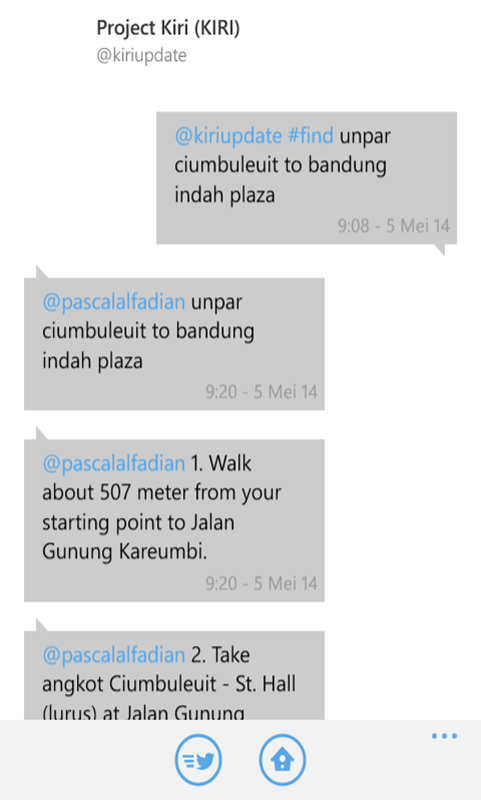
\includegraphics{Gambar/contohpercakapan}
	\label{fig:contohpercakapan}
\end{figure}

\section{Rumusan Masalah}
Mengacu kepada deskripsi yang diberikan, maka rumusan masalah pada penelitian ini adalah:
\begin{itemize}
	\item Bagaimana membuat \textit{Twitter bot} untuk mencari jalur transportasi publik?
	\item Bagaimana membuat \textit{Twitter bot} untuk dapat merespon secara real time?
	\item Bagaimana memformat petunjuk rute perjalanan dalam keterbatasan tweet 140 karakter?
\end{itemize}

\section{Tujuan}
Tujuan dari penelitian ini adalah:
\begin{itemize}
	\item Membuat aplikasi \textit{Twitter bot} untuk mencari jalur transportasi publik.
	\item Membuat aplikasi Twitter yang bekerja secara \textit{real time}.
	\item Membuat algoritma untuk memecah instruksi dari KIRI API dan mengubahnya ke dalam bentuk tweet.
\end{itemize}

\section{Batasan Masalah}
Pada pembuatan perangkat lunak ini, masalah-masalah yang ada akan dibatasi menjadi:
\begin{itemize}
	\item Input hanya mencakup Kota Bandung saja.
	\item Input yang diinputkan harus benar, memiliki asal dan tujuan yang jelas di Kota Bandung.
	\item Hasil yang dikeluarkan berupa tweet jalur transportasi publik.
	\item Media transportasi publik yang digunakan adalah angkutan umum.
	\item Pencarian jalur memanfaatkan KIRI API.
\end{itemize}

\section{Metode Penelitian}
Pada perangkat lunak yang dibuat ini digunakan beberapa metode dalam penyelesaian masalah yang menjadi topik pada penelitian ini, antara lain:
\begin{itemize}
	\item Pada saat mengambil kuliah AIF401 Skripsi 1
	\begin{enumerate}
		\item Melakukan studi literatur, antara lain:
		\begin{itemize}
			\item KIRI API,
			\item REST API Twitter (https://dev.twitter.com/docs/api/1.1),
			\item Streaming API Twitter (https://dev.twitter.com/docs/api/streaming).
		\end{itemize}
		\item Mempelajari pembuatan server dalam bahasa Java.
		\item Mencoba membuat \textit{Twitter bot} sederhana.
		\item Membuat laporan dalam bentuk skripsi.
		\item Melakukan analisis terhadap teori-teori yang sudah dipelajari, guna membangun perangkat lunak yang dimaksud.
	\end{enumerate}
	\item Pada saat mengambil kuliah AIF401 Skripsi 2
	\begin{enumerate}
		\item Merancang perangkat lunak \textit{Twitter bot}.
		\item Mengimplementasi perangkat lunak \textit{Twitter bot}.
		\item Mengimplementasikan pembangkit \textit{Twitter bot}. 
		\item Melakukan pengujian dan eksperimen.
		\item Membuat dokumentasi skripsi.
	\end{enumerate}
\end{itemize}.
}{}
\ifdefstring{\vbaba}{1}{\chapter{Dasar Teori}
\label{chap:dasar teori}

Sebelum bisa membuat \textit{Twitter bot} untuk mencari jalur transportasi publik, berikut diberikan beberapa definisi yang berkaitan dengan pembuatan \textit{Twitter bot}. Bab ini akan menjelaskan Twitter, Twitter API, KIRI, KIRI API, dan Twitter4j.

\section{Twitter \cite{TwitterBook}}
\label{sec:twitter}

Twitter adalah salah satu layanan jejaring sosial yang memungkinkan pengguna melakukan \textit{posting} pesan berbasis teks hingga 140 karakter. Berikut ini adalah daftar istilah umum pada Twitter:


\begin{itemize}
	\item \textit{Tweet} 
	
	Posting pada Twitter disebut sebagai \textit{tweet}. \textit{Tweet} ini akan meneruskan pesan singkat yang ditujukan ke semua \textit{follower} suatu akun. Contohnya adalah seorang akun @kviniink ingin menuliskan bahwa hari ini cuaca cerah, maka akun @kviniink akan melakukan \textit{tweet} 'Hari ini cerah yah..'. \textit{Tweet} juga bisa menyertakan \textit{link} untuk video, foto, atau media lain di internet selain teks biasa. URL(\textit{Uniform resource locator}) \textit{link} teks termasuk ke dalam 140 batas karakter, namun URL tersebut akan menghabisnya tempat/\textit{space} dari keterbatasan karakter \textit{tweet}. Oleh karena itu, URL akan dibuat versi singkatnya, contohnya pada saat pengguna memasukkan \textit{link} \url{http://www.chacha.com/gallery/7253/15-movies-that-make-guys-cry}, maka \textit{link} tersebut akan dibuat menjadi \url{bit.ly/1uRi8vV}. 
	\item \textit{Follow}
	
	\textit{Follow} adalah satu istilah dalam Twitter yang bertujuan untuk mengikuti aktivitas \textit{tweet} suatu akun. \textit{Following} adalah ketika sebuah akun mengikuti akun orang lain, dan \textit{Follower} adalah ketika sebuah akun melakukan aksi \textit{follow} kepada akun anda.
	\item \textit{Reply} 
	
	\textit{Reply} adalah cara seseorang untuk dapat memberi rujukan kepada akun Twitter yang lainnya atau lebih dikenal dengan nama \textit{mention}. Sebagai contoh, diketahui akun bernama @kviniink mem-\textit{follow} @infobdg untuk mengetahui perkembangan apa saja yang tejadi di Kota Bandung. Lalu akun @kviniink ingin bertanya tentang info \textit{mall} yang sedang ramai dikunjungi di Kota Bandung, maka akun @kviniink membuat \textit{mention tweet} yang berisikan "@infobdg Halo saya ingin bertanya apa saja \textit{mall} yang sedang ramai dikunjungi di Bandung yah?". Setelah akun @infobdg membaca \textit{mention} dari @kviniink, akun @infobdg melakukan balasan kepada akun @kviniink untuk membalas pertanyaan yang diajukan oleh akun @kviniink. \textit{Tweet} tersebut berisikan "@kviniink mungkin anda bisa mengunjungi PVJ dan Ciwalk".
	\item \textit{Retweet}
	
	\textit{Retweet} ini merupakan salah satu istilah penting dari Twitter. \textit{Retweet} ini berguna ketika pengguna menemukan \textit{tweet} menarik dan ingin  berbagi \textit{tweet} tersebut dengan \textit{follower} akun tersebut. \textit{Retweet} ini juga secara tidak langsung mengatakan bahwa "saya menghormati anda dan pesan yang anda buat". Contohnya adalah ketika akun @infobdg melakukan \textit{tweet} tentang penutupan jalan di Bandung dan suatu akun ingin membagian informasi tersebut kepada \textit{follower} mereka. Maka akun tersebut akan melakukan \textit{retweet} terhadap \textit{tweet} yang diposting oleh akun @infobdg.
	\item \textit{Hashtag}
	
	Sebuah fitur yang diciptakan oleh Twitter untuk membantu pencarian kata kunci dan penandaan suatu diskusi. Contohnya adalah ketika suatu akun mendatangi suatu acara bernama IXPO, dan akun tersebut ingin memposting \textit{tweet} tentang IXPO tersebut, maka akun tersebut dapat menuliskan \#IXPO pada \textit{tweet} yang diposting.
	
	\item \textit{Direct Message}(DM)
	
	\textit{Direct message} digunakan untuk mengirim pesan yang bersifat \textit{private} antara dua akun Twitter. Syarat agar dapat melakukan \textit{direct message} adalah melakukan aksi \textit{follow} terhadap akun yang akan dikirimkan \textit{direct message}.
	\item \textit{Timeline}
	
	\textit{Timeline} adalah sekumpulan \textit{tweet} dari semua akun yang di-\textit{follow}. \textit{Timeline }ditampilkan di halaman utama.
\end{itemize}


\section{Twitter API \cite{Twitter}}
Twitter API(\textit{Application programming interface}) adalah aplikasi pihak ketiga yang memungkinkan pengembang perangkat lunak melakukan manipulasi dan pengolahan data di Twitter. Twitter API adalah salah satu bentuk pendekatan dari Twitter yang berfokus pada jaringan dan memungkinkan pengembang perangkat lunak memiliki hak untuk berpikir '\textit{out of the box}' untuk membuat aplikasi yang mereka inginkan\cite{Twitter}. Tetapi tetap akan terjadi keterbatasan yang dimiliki Twitter API, yaitu :
\begin{itemize}
	\item Hanya bisa melakukan \textit{tweet} 1000 per harinya, baik melalui \textit{handphone}, \textit{website}, API, dan sebagainya.
	\item Total pesan hanya bisa sebanyak 250 per harinya, pada setiap dan semua perangkat.
	\item 150 permintaan API per jam.
\end{itemize}

\subsection{\textit{Search} API}

Twitter \textit{Search} API memungkinkan melakukan pencarian terhadap \textit{tweet} baru ataupun \textit{tweet} populer. Tetapi Twitter \textit{Search} API ini bukan fitur yang tersedia pada \textit{website} Twitter itu sendiri. API ini difokuskan kepada relevansi, bukan terhadap kelengkapan data\cite{Twitter}. Ini berarti bahwa ada beberapa \textit{Tweet} atau akun akan hilang dari hasil pencarian.

\paragraph{Bagaimana cara membuat sebuah \textit{query}}
Cara terbaik dalam membuat sebuah \textit{query} adalah melakukan percobaan yang valid dan mengembalikan \textit{tweet} yang sesuai. Cara mencobanya dapat dilakukan pada \url{twitter.com/search}. URL yang ditampilkan pada \textit{browser} akan berisi sintaks \textit{query} yang sesuai agar dapat digunakan kembali pada Twitter API. Berikut adalah contohnya:

\begin{enumerate}
	\item Melakukan pencarian untuk \textit{tweet} yang di-\textit{mention} kepada akun @twitterapi. Pencarian dilakukan pada \url{twitter.com/search}.
	\item Lakukan pengecekan dan salin URL yang ditampilkan pada browser. Sebagai contoh didapatkan URL seperti \url{https://twitter.com/search?q=\%40twitterapi}.
	\item Ganti \url{https://twitter.com/search} dengan \url{https://api.twitter.com/1.1/search/tweets.json} dan akan didapatkan \url{https://api.twitter.com/1.1/search/tweets.json?q=\%40twitterapi}
	\item Eksekusi URL tersebut untuk melakukan pencarian di dalam API.
\end{enumerate}

API v1.1 mewajibkan \textit{request} yang sudah diotentikasi. Perlu diingat juga bahwa hasil pencarian yang dilakukan di \url{twitter.com} dapat menghasilkan data yang sudah sangat lama, sedangkan \textit{Search} API hanya melayani \textit{tweet} dari seminggu terakhir. Contoh berbagai macam pencarian dapat dilihat pada tabel \ref{tab:MacamPencarianTweet}:

\begin{table}[h]
\caption{Contoh berbagai macam pencarian \textit{tweet}}
\label{tab:MacamPencarianTweet}
\begin{tabular}{|p{5cm}|p{9cm}|}
\hline
\textbf{Operator}          					& \textbf{Finds \textit{tweets}}                                            \\ \hline
\textit{watching now}               & Mengandung kata "\textit{watching}" dan "\textit{now}".						       \\
"\textit{happy hour}"               & Mengandung frase "\textit{happy hour}" yang tepat.                                 \\
\textit{love OR hate}               & Mengandung kata "\textit{love}" atau "\textit{hate}" atau keduanya.                             \\
\textit{beer -root}                 & Mengandung kata "\textit{beer}" tanpa adanya kata "\textit{root}".                                         \\
\#haiku                    					& Mengandung \textit{hashtag} "\textit{haiku}".                                            \\
\textit{from}:alexiskold            & Dikirim melalui akun "alexiskold".                                            \\
\textit{to}:techcrunch              & Dikirimkan kepada akun "techcrunch".                                              \\
@mashable                  					& Mereferensi kepada akun "mashable".                                            \\
\textit{superhero since}:2010-12-27 & Mengandung kata "\textit{superhero}" dari tanggal "2010-12-27" (tahun-bulan-hari). \\
\textit{ftw until}:2010-12-27       & Mengandung kata "\textit{ftw}" sebelum tanggal "2010-12-27".                   \\
\textit{movie -scary} :)            & Mengandung kata "\textit{movie}", tanpa adanya kata "\textit{scary}", dengan pencarian yang positif.        \\
\textit{flight} :(                  & Mengandung kata "\textit{flight}" dengan pencarian yang negatif.                         \\
\textit{traffic} ?                  & Mengandung kata "\textit{traffic}" dan mengandung pertanyaan.                               \\
\textit{hilarious filter:links}     & Mengandung kata "\textit{hilarious}" yang di sambungkan dengan URL.                                \\
\textit{news source:twitterfeed}    & Mengandung kata "\textit{news}" yang di-\textit{posting} melalui \textit{twitterfeed}.						\\        \hline                     
\end{tabular}
\end{table}

Dipastikan bahwa pengkodean URL terhadap \textit{query} dilakukan terlebih dahulu sebelum melakukan \textit{request}. Tabel \ref{tab:ContohMappingDariSeachQuery} memberikan contoh \textit{mapping} dari \textit{search query} ke \textit{query} pengkodean URL.

\begin{table}[h]
\caption{Contoh \textit{mapping} dari \textit{search query} ke \textit{query} pengkodean URL}
\label{tab:ContohMappingDariSeachQuery}
\begin{tabular}{|l|l|}
\hline
\textbf{\textit{Search query}}     & \textbf{\textit{URL encoded query}}                 \\ \hline
\#haiku \#poetry & \%23haiku+\%23poetry              \\
"\textit{happy hour}" :)  & \%22\textit{happy}\%20\textit{hour}\%22\%20\%3A\%29 \\ \hline
\end{tabular}
\end{table}

\paragraph{\textit{Additional parameters}}
Terdapat parameter tambahan yang dapat digunakan untuk menghasilkan pencarian yang lebih baik. Berikut adalah penjelasan dari parameter tambahan tersebut :

\begin{itemize}
	\item \textbf{\textit{Result Type}}. Seperti hasil yang terdapat pada \url{twitter.com/search}, parameter \textit{result\_type} memungkinkan hasil pencarian akan berdasarkan \textit{tweet} yang paling baru atau \textit{tweet} yang paling populer atau bahkan gabungan dari keduanya.
	\item \textit{\textbf{Geolocatization}}. Pencarian tempat tidak tersedia pada API, tetapi ada beberapa cara yang tepat untuk membatasi \textit{query} dengan cara menggunakan parameter \textit{geocode} lalu menentukan "\textit{latitude, longitude, radius}". Contohnya adalah "37.781157,-122.398720,1mi". Ketika pencarian lokasi, pencarian API akan mencoba menemukan \textit{tweet} yang memiliki \textit{latitude} dan \textit{longitude} yang sudah dimasukkan kedalam \textit{query geocode}, jika tidak berhasil maka API akan mencoba menemukan \textit{tweet} yang dibuat oleh pengguna yang lokasi profilenya terdapat pada \textit{latitude} dan \textit{longitude} tersebut. Kesimpulannya adalah hasil pencarian dapat menerima \textit{tweet} yang tidak mencakup informasi \textit{latidute} atau \textit{longitude}.
	\item \textit{\textbf{Language}}. Bahasa dapat dijadikan parameter untuk mencari \textit{tweet} yang sesuai dengan bahasa yang dipilih.
	\item \textbf{\textit{Iterating in a result set}}. Parameter seperti \textit{count, until, since\_id, max\_id} memungkinkan untuk melakukan kontrol bagaimana iterasi melalui hasil pencarian.
\end{itemize}

\paragraph{\textit{Rate limits}}
\textit{User} pada saat ini diwakilkan oleh \textit{access tokens} yang dapat membuat 180 \textit{request} per 15 menit. Tetapi pengguna bisa membuat 450 \textit{request} per 15 menit dengan menggunakan \textit{application-only authentication} atas nama sendiri tanpa konteks pengguna.

\paragraph{Contoh Pencarian}
Ketika anda mengikuti suatu acara yaitu \textit{superbowl}, lalu anda tertarik untuk mencari hal yang sedang terjadi di acara tersebut dengan melihat \textit{tweet} yang paling baru dan menggunakan \textit{hashtag} dari acara tersebut, maka langkah-langkah yang dilakukan adalah:
\begin{itemize}
	\item Anda ingin mencari \textit{tweet} yang paling baru dengan menggunakan \textit{hashtag} \#\textit{superbowl}
	\item Maka \textit{search} URL akan seperti ini:
	\url{https://api.twitter.com/1.1/search/tweets.json?q=\%23superbowl\&result\_type=recent}
\end{itemize}

Ketika anda ingin mengetahui \textit{tweet} yang datang dari suatu lokasi dengan bahasa yang spesifik, maka langkah-langkah yang dilakukan adalah:
\begin{itemize}
	\item Anda ingin mencari \textit{tweet} yang paling baru dalam Bahasa Portugal, yang lokasinya dekat Maracana soccer stadium yang terletak di Rio de Janeiro.
	\item Maka search URL akan seperti ini:
	\url{https://api.twitter.com/1.1/search/tweets.json?q=\&geocode=-22.912214,-43.230182,1km\&lang=pt\&result\_type=recent}
	
Ketika anda ingin mencari \textit{tweet} yang sedang poluler dari spesifik \textit{user} dan \textit{tweet} tersebut terdapat sebuah hashtag tertentu, maka langkah-langkah yang dilakukan adalah:
\begin{itemize}
	\item Anda ingin mencari \textit{tweet} yang populer yang berasal dari \textit{user} @kviniink yang terdapat \textit{hashtag} \#nasa.
	\item Maka \textit{search} URL akan seperti ini:
	\url{https://api.twitter.com/1.1/search/tweets.json?q=from\%3Akviniink\%20\%23nasa\&result\_type=popular}
\end{itemize}
\end{itemize}

\subsection{Streaming API}
\textit{Streaming} API adalah contoh \textit{real-time} API. API ini ditujukan bagi para developer dengan kebutuhan data yang intensif. \textit{Streaming} API memungkinkan melacak kata kunci yang ditentukan dalam jumlah besar dan melakukan suatu aksi (seperti \textit{tweet}) secara langsung atau \textit{real-time}.

Twitter menawarkan beberapa \textit{endpoint streaming}, disesuaikan dengan kasus yang dibutuhkan. 
\begin{itemize}
	\item \textit{Public stream}
	
	\textit{Public stream} merupakan \textit{streaming} data publik yang mengalir melalui Twitter. \textit{Public stream} Digunakan untuk mengikuti sebuah \textit{user} atau topik tertentu. \textit{Public stream} biasa  digunakan untuk \textit{data mining}.
	\item \textit{User Stream}
	
	{User Stream} merupakan \textit{Single-user streams} yang mengandung hampir semua data yang berhubungan dengan satu \textit{user} tertentu.
	
	\item \textit{Site Stream}
	
	\textit{Site Stream} merupakan versi dari \textit{multi-user stream}. \textit{Site stream} terhubung dengan server yang terkoneksi dengan Twitter atas nama banyak pengguna.
\end{itemize}


\paragraph{\textit{Public Streams}}
\textit{Stream} ini menawarkan sampel data publik yang mengalir melalui Twitter. Ketika aplikasi membuat sambungan ke \textit{streaming endpoint}, perangkat lunak akan mengambil \textit{tweet} tanpa perlu khawatir akan keterbatasan \textit{rate limit}.

\paragraph{\textit{Endpoints}}
	
	\begin{itemize}
		\item POST statuses / \textit{filter}
		\item GET statuses / \textit{sample}
		\item GET statuses / \textit{firehose}
	\end{itemize}

\paragraph{POST statuses/\textit{filter}}
POST \textit{filter} dapat mengembalikan status publik yang sesuai dengan satu atau lebih predikat yang telah difilter. \textit{Multiple parameter} memungkinkan klien untuk menggunakan koneksi tunggal untuk ke \textit{Streaming} API. Antara GET \textit{request} dan POST \textit{request} keduanya didukung oleh POST statuses / \textit{filter} tetapi untuk GET \textit{request} yang memiliki parameter yang terlalu banyak mungkin akan ditolak karena URL yang terlalu panjang. Gunakanlah POST request untuk menghindari URL yang panjang.
\textit{Track, follow}, dan lokasi harus dipertimbangkan untuk dapat digabungkan dengan operator OR. \textit{track}=foo\&\textit{follow}=1234 ini mengembalikan \textit{tweet} yang memiliki kata "foo" atau dibuat oleh \textit{user} 1234.
Akses standar mengizinkan pencarian hingga 400 kata kunci, dan 5000 \textit{follow userids}. Perintah ini dikembalikan dalam format JSON, memerlukan otentikasi \textit{user context}, dan frekuensi pemakaiannya dibatasi. Parameter untuk POST statuses/\textit{filter} dapat dilihat pada tabel \ref{table:ParameterPostStatusesFilter}

%\paragraph{\textit{Resource Information}}
%\begin{table}[!htbp]
%\begin{tabular}{|l|l|}
%\hline
%\textit{Response formats}         & JSON                    \\ \hline
%\textit{Requires authentication}? & Ya (hanya \textit{user context}) \\ \hline
%\textit{Rate limited}?            & Ya                    \\ \hline
%\end{tabular}
%\end{table}


\begin{table}[h]
\caption{Parameter POST statuses/\textit{filter}}
\label{table:ParameterPostStatusesFilter}
\begin{tabular}{|p{3cm}|p{11cm}|}
\hline
\textit{follow}          & Menentukan pencarian \textit{tweet} dari suatu akun. \\ \hline
\textit{track}           & Kata kunci pencarian untuk di-\textit{track}.              \\ \hline
\textit{locations}       & Menentukan lokasi yang dilacak.                                                    \\ \hline
\textit{delimited}       & Menentukan apakah pesan harus dibatasi limitnya.                                         \\ \hline
\textit{stall\_warnings} & Menentukan apakah pesan warning harus dikirim atau tidak. \\ \hline                                        
\end{tabular}
\end{table}


\paragraph{GET \textit{statuses/sample}}
Mengembalikan \textit{random} sampel dari semua status publik. Jika terdapat dua \textit{client} yang terhubung dengan \textit{endpoint} ini, maka kedua \textit{client} tersebut akan melihat \textit{tweet} yang sama. Perintah ini dikembalikan dalam format JSON, memerlukan otentikasi \textit{user context}, dan frekuensi pemakaiannya dibatasi. Parameter GET \textit{statuses/sample} dapat dilihat pada tabel \ref{table:ParameterGetStatusesSample}

\begin{table}[h]
\caption{Parameter GET \textit{statuses/sample}}
\label{table:ParameterGetStatusesSample}
\begin{tabular}{|l|l|}
\hline
\textit{delimited}          & Menentukan apakah pesan harus dibatasi limitnya. \\ \hline
\textit{stall\_warning}           & Menentukan apakah pesan warning harus dikirim atau tidak.                \\   \hline          
\end{tabular}
\end{table}


\paragraph{GET \textit{statuses/firehose}}
Mengembalikan semua status publik. Beberapa aplikasi membutuhan akses ini. Teknik ini diolah secara kreatif dengan cara menggabungkan sumber informasi yang ada dengan berbagai sumber lainnya untuk dapat memuaskan pengguna. Perintah ini dikembalikan dalam format JSON, memerlukan otentikasi \textit{user context}, dan frekuensi pemakaiannya dibatasi. Parameter GET \textit{statuses/firehose} dapat dilihat pada tabel \ref{table:ParameterGetStatusesFirehose}


\begin{table}[h]
\caption{Parameter GET \textit{statuses/firehose}}
\label{table:ParameterGetStatusesFirehose}
\begin{tabular}{|l|l|}
\hline
\textit{count} & Kumpulan pesan untuk dijadikan bahan materi \\ \hline
\textit{delimited}          & Menentukan apakah pesan harus dibatasi limitnya. \\ \hline
\textit{stall\_warning}           & Menentukan apakah pesan warning harus dikirim atau tidak.                \\     \hline        
\end{tabular}
\end{table}


\paragraph{Menggunakan \textit{Streaming} API}
Proses menggunakan \textit{streaming} API adalah dengan cara menghubungkan \textit{endpoint} yang sudah tercantum di atas dengan parameter yang sudah di-\textit{list} kepada \textit{streaming endpoint} dan juga \textit{request} parameter \textit{streaming} API.

\paragraph{Koneksi}
Setiap akun hanya dapat membuat satu koneksi yang terhubung dengan \textit{public endpoint} dan jika melakukan koneksi ke \textit{public stream} lebih dari satu kali dengan menggunakan akun yang sama akan menyebabkan koneksi terlama akan putus. Klien yang membuat koneksi secara berlebihan baik berhasil ataupun tidak maka IP mereka otomatis akan di \textit{banned}.

%User Streams
\paragraph{\textit{User Streams}}
\textit{User Stream} memberikan aliran(\textit{stream}) data dan event yang spesifik untuk akun yang sudah diotentikasi. Perintah ini dikembalikan dalam format JSON, memerlukan otentikasi \textit{user context}, dan frekuensi pemakaiannya dibatasi. Parameter untuk parameter ini dapat dilihat pada tabel \ref{table:ParameterGetUser}


\paragraph{\textit{Endpoints}}
\begin{itemize}
	\item GET \textit{user}
\end{itemize}

\begin{table}[h]
\caption{Parameter GET \textit{user}}
\label{table:ParameterGetUser}
\begin{tabular}{|p{5cm}|p{9cm}|}
\hline
\textit{delimited}              & Menentukan apakah pesan harus dibatasi limitnya.																												\\ \hline
\textit{stall\_warnings}        & Menentukan apakah pesan \textit{warning} harus dikirim atau tidak.                                                               \\ \hline
\textit{with}                   & Menentukan apakah pesan informasi harus dikembalikan kepada akun yang sudah diotentikasi atau dilakukan pengiriman juga kepada akun yang di-\textit{follow} oleh akun yang sudah diotentikasi tersebut.\\ \hline
\textit{replies}                & Menentukan apakah harus mengembalikan @replies.                                                                             \\ \hline
\textit{follow}                 & Termasuk \textit{tweet publik} tambahan dari daftar yang disediakan untuk ID pengguna.														\\ \hline
\textit{track}                  & Termasuk \textit{tweet} tambahan yang cocok dengan kata kunci tertentu.     \\ \hline
\textit{locations}              & Termasuk \textit{tweet} tambahan yang termasuk dalam batasan lokasi tertentu.                                                      \\ \hline
\textit{stringify\_friend\_ids} & Mengirim list teman yang terdiri dari \textit{array of integer} dan \textit{array of string}.              \\ \hline            
\end{tabular}
\end{table}

\paragraph{Koneksi}
Jika suatu perangkat lunak menggunakan \textit{user stream}, maka sebisa mungkin untuk meminimalkan jumlah koneksi suatu perangkat lunak. Setiap akun Twitter terbatas hanya untuk beberapa koneksi \textit{user stream} per otentikasi perangkat lunak, terlepas dari IP(\textit{Internet Protocol}). Setelah mencapai batasnya, maka koneksi tertua atau terlama akan diberhentikan secara otomatis. \textit{User} \textit{login} dari beberapa instansi dari otentikasi perangkat lunak yang sama akan mengalami siklus koneksi yaitu akan dihubungan dan diputuskan satu sama lain.

Sebuah aplikasi harus dapat mengatasi HTTP(\textit{The Hypertext Transfer Protocol}) 420 \textit{error code} yang memberitahukan bahwa suatu akun sudah terlalu sering melakukan \textit{login}. Oleh karena itu, akun yang seperti itu akan secara otomatis di-\textit{banned} dari \textit{user stream} untuk tingkat \textit{login} yang berlebihan. Perhatikan bahwa setiap perangkat lunak memiliki alokasinya masing-masing, sehingga \textit{login} dari perangkat lunak yang pertama tidak akan mempengaruhi koneksi untuk perangkat lunak yang kedua, begitu juga sebaliknya. Tetapi akan menimbulkan masalah apabila menjalankan terlalu banyak salinan perangkat lunak yang pertama maupun kedua. Jika anda perlu membuat koneksi atas nama beberapa akun dari perangkat lunak yang sama, maka akan lebih baik jika menggunakan \textit{site stream}.

%OAuth
\section{OAuth}
\label{sec:oauth}
Dengan semakin berkembangnya \textit{website}, semakin banyak situs yang bergantung pada layanan distribusi dan \textit{cloud computing}. Contohnya adalah menggunakan jejaring sosial dengan menggunakan akun media sosial lainnya seperti Google untuk mencari teman-teman yang sudah tersimpan pada kontak Google. Atau bisa juga menggunakan pihak ketiga yang memanfaatkan API dari beberapa layanan.

OAuth menyediakan suatu metode bagi pengguna untuk memberi akses pihak ketiga untuk \textit{resources} (sumber daya) client tanpa berbagi \textit{password}. Sebagai contoh, seorang pengguna \textit{website} dapat memberikan layanan percetakan untuk mengakses foto pribadinya yang disimpan di layanan berbagi foto tanpa harus memberikan \textit{username} dan \textit{password}nya. Ia akan mengotentikasi langsung dengan layanan berbagi foto tersebut sehingga dapat dibagikan kepada layanan percetakan.

Agar \textit{client} dapat mengakses \textit{resource}, pertama-tama client harus mendapatkan izin dari si pemilik \textit{resource}. Izin ini dinyatakan dalam bentuk token dan juga digunakan untuk mencocokkan \textit{shared-secret}. Tujuan dari token ini adalah untuk membuat pemilik \textit{resource} berbagi kepercayaan mereka kepada \textit{client}. Token dapat dikeluarkan dalam ruang lingkup terbatas, durasi yang terbatas, dan akan dicabut secara independen\footnote{Hueniverse Documentation , OAuth, \url{http://hueniverse.com/oauth/guide/intro/}, pada tanggal 20 Agustus 2014 pukul 12.58}.

\paragraph{Twitter OAuth}yang diberikan memiliki fitur :
\begin{itemize}
	\item \textit{Secure}
	
	Pengguna tidak harus berbagi \textit{password} mereka dengan aplikasi pihak ketiga untuk meningkatkan keamanan akun.
	\item \textit{Standard}
	
	Banyak \textit{library} dan contoh kode yang tersedia dengan implementasi Twitter Oauth.
\end{itemize}

Twitter API mengijinkan 350 permintaan OAuth per jam.

\subsection{\textit{Application-only authentication}}
Twitter menawarkan aplikasi yang mampu mengeluarkan permintaan otentikasi atas nama aplikasi itu sendiri. Dengan menggunakan \textit{application-only authentication}, perangkat lunak tidak mempunyai konteks dari otentikasi pengguna dan ini berarti setiap \textit{request} API untuk endpoint akan membutuhkan konteks pengguna, seperti memposting \textit{tweet} tidak akan bekerja. \textit{Application-only authentication} dapat melakukan berbagai macam aktivitas, seperti : 

\begin{itemize}
	\item melihat \textit{timeline}, 
	\item mengakses \textit{following} dan \textit{follower} dari suatu \textit{akun},
	\item mencari \textit{tweet},
	\item mengambil informasi dari akun Twitter manapun.
\end{itemize}


Tetapi \textit{application-only authentication} tidak dapat melakukan :

\begin{itemize}
	\item Posting \textit{tweet}
	\item Melakukan koneksi dengan \textit{Streaming endpoint}
	\item Mencari akun seseorang
	\item Menggunakan \textit{geo endpoint}
	\item Mengakses \textit{Direct Message}
\end{itemize}

\paragraph{\textit{OAuth Flow}}
Langkah-langkah dari \textit{application-only auth} terdiri dari :
Sebuah aplikasi dikodekan berdasarkan \textit{consumer key} dan \textit{secret} ke dalam satu set khusus yang dikodekan secara kredensial.
aplikasi membuat \textit{request} kepada POST OAuth2/\textit{token endpoint} untuk mengubah kredensial tersebut menjadi \textit{token bearer}.
Ketika mengakses REST API, aplikasi menggunakan \textit{token bearer} untuk melakukan otentikasi.

\paragraph{Tentang \textit{Application-only Authentication}}
Token adalah \textit{password}. \textit{Consumer key} dan \textit{secret, bearer token credential}, dan \textit{the bearer token} memberikan akses untuk membuat permintaan atas nama aplikasi itu sendiri. Poin-poin ini harus dianggap sensitif layaknya \textit{password} dan tidak boleh dibagikan atau didistribusikan kepada pihak yang tidak dipercaya atau tidak berkepentingan.

\textit{SSL}(\textit{Secure Sockets Layer}) sangat dibutuhkan karena \textit{SSL} merupakan cara otentikasi yang aman. Oleh karena itu, semua \textit{request} (baik untuk mendapatkan atau menggunakan token) harus menggunakan \textit{endpoint} HTTPS, yang juga merupakan syarat untuk menggunakan API.

\textit{Request} yang dibuat atas nama pengguna tidak akan menguras ketersediaan \textit{rate limit}, begitu juga dengan \textit{request}. Request tidak akan menguras batas penggunaan \textit{limit} dalam \textit{user-based auth}.


\subsection{3-\textit{legged authorization}}
Tahap awal dari cara kerja dari \textit{3-legged authorization} adalah dengan memberikan \textit{access token}. Pengambilan \textit{access token} dilakukan dengan cara melakukan \textit{redirect} akun dengan Twitter. Lalu Twitter memberikan akun sebuah otentikasi dari aplikasi yang telah dibuat. Terdapat dua pengecualian dalam cara kerja dari \textit{3-legged authorization}, yaitu :

\begin{itemize}
	\item GET \textit{oauth endpoint} digunakan sebagai pengganti GET \textit{oauth},
	\item akun akan selalu diminta untuk mengotentikasi perangkat lunak.
\end{itemize}

\subsection{\textit{PIN-based authorization}}
\textit{PIN-based authorization} ditujukan untuk perangkat lunak yang tidak bisa mengakses atau menanamkan \textit{web browser} untuk mengarahkan akun kepada \textit{authorization endpoint}. Contohnya adalah perangkat lunak yang bersifat \textit{command-line}, \textit{embedded systems}, \textit{game} konsol, dan beberapa jenis aplikasi \textit{mobile}.


\paragraph{Implementasi}

Implementasi \textit{PIN-based authorization} ini memiliki cara kerja yang sama seperti \textit{3-legged authorization}. Perbedaan antara \textit{PIN-based authorization} dengan 3-\textit{legged authorization} terletak pada nilai dari \textit{oauth\_callback} yang harus di-set menjadi \textit{oob} saat proses pemanggilan \textit{POST oauth} atau \textit{request\_token}.

Setelah perangkat lunak telah mendapatkan \textit{GET oauth/authenticate} atau \textit{GET oauth/authorize URL}, aplikasi akan memberi URL kepada pengguna. URL tersebut dimasukkan oleh pengguna menggunakan \textit{web browser} untuk mengakses URL tersebut.

Ketika \textit{callback oob} diminta, pengguna tidak akan dipindahkan secara otomatis ke perangkat lunak setelah menyetujui akses seperti yang dilakukan 3-\textit{legged authorization}. Akan tetapi jika menggunakan \textit{PIN-based authorization}, pengguna akan melihat kode PIN untuk dikembalikan kepada perangkat lunak dengan cara memasukkan nilai dari kode PIN yang sudah diberikan. Gambar~\ref{fig:pin} merupakan contoh nilai kode yang diberikan.

\begin{figure}[H]
\centering
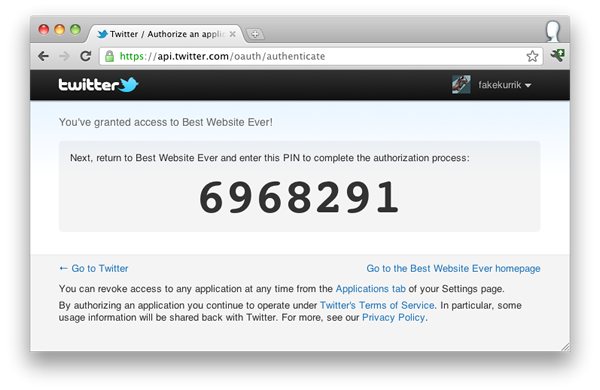
\includegraphics{Gambar/pin.png}
\caption{Contoh PIN-based authorization}
	\label{fig:pin}
\end{figure}

Perangkat lunak harus dirancang agar memungkinkan pengguna untuk memasukkan \textit{PIN code}. Nilai dari \textit{PIN code} harus lolos sebagai \textit{oauth\_verifier} untuk \textit{POST oauth/access\_token request}. Semua \textit{request} akan berjalan normal kedepannya.

\section{JSON\cite{Json}}
JSON(\textit{JavaScript Object Notation}) adalah suatu format pertukaran data komputer berbasis teks. JSON digunakan untuk merepresentasikan struktur data sederhana karena formatnya mudah dibaca oleh manusia. Selain itu juga format JSON mudah digunakan oleh suatu perangkat lunak  untuk melakukan \textit{parse} dan \textit{generate}. JSON didasarkan pada subset bahasa pemrograman \textit{JavaScript}. JSON dianggap sebagai format data yang tak tergantung pada suatu bahasa. Beberapa bahasa pemograman telah menyediakan \textit{library} untuk pengolahan data JSON.

JSON dibangun dengan dua struktur, yaitu:
\begin{enumerate}
	\item Nama. Nama ini direalisasikan sebagai objek, \textit{record}, kamus, tabel \textit{hash}, \textit{keyed list}, atau \textit{associative array}.
	\item Nilai. Nilai ini direalisasikan sebagai \textit{array}, vektor, \textit{list}, atau \textit{sequence}.
\end{enumerate}

Listing ~\ref{lst:DataSeorangMahasiswaUNPAR} menunjukkan representasi JSON untuk suatu objek yang mendeskripsikan seseorang mahasiswa UNPAR.

\begin{lstlisting} [caption= {Data Seorang Mahasiswa UNPAR},label={lst:DataSeorangMahasiswaUNPAR}]
{ 
    {
     "namaDepan": "Kevin",
     "namaBelakang": "Theodorus",
		 "NPM" : "2011730037",
		 "Jurusan" : "Teknik Informatika"
     "alamat": {
         "namaJalan": "Jl. Mekar Sederhana 17",
         "kota": "Bandung",
         "kodePos": 40237
     },
     "nomerTelepon": [ 
         "089676821932",
				 "5233901"
     ]
		}
}
\end{lstlisting} 
Listing ~\ref{lst:DataSeorangMahasiswaUNPAR} menunjukan data seorang mahasiswa UNPAR. Berikut ini adalah keterangan dari data seorang mahasiswa UNPAR tersebut:
\begin{itemize}
	\item Index 0 berisikan nama depan dari mahasiswa UNPAR. Nilai dari nama depan adalah Kevin.
	\item Index 1 berisikan nama belakang dari mahasiswa UNPAR. Nilai dari nama belakang adalah Theodorus.
	\item Index 2 berisikan NPM(Nomor Pokok Mahasiswa) dari mahasiswa UNPAR. Nilai dari NPM adalah 2011730037.
	\item Index 3 berisikan alamat dari mahasiswa UNPAR. Objek alamat memiliki tiga \textit{string} yaitu nama jalan, kota, dan kode pos. Nilai dari \textit{string} nama jalan adalah Jl. Mekar Sederhana 17, nilai dari \textit{string} kota memiliki nilai Bandung, dan \textit{string} dari kode pos memiliki nilai 40237.
	\item Index 4 berisikan nomor telepon dari mahasiswa UNPAR. Nomor telepon memiliki nilai \textit{array}, nilai yang pertama adalah 089676821932 dan nilai yang ke dua adalah 5233901.
\end{itemize}

\section{KIRI API\cite{Kiri}}
KIRI API adalah aplikasi pihak ketiga yang memungkinkan pengembang perangkat lunak mendapatkan data tentang info jalur transportasi publik. Semua \textit{request} harus berisi API \textit{key} yang dapat diambil melalui KIRI API \textit{Management Dashboard}. Berikut adalah spesifikasi dari KIRI API :

\begin{itemize}
	\item \textit{Routing Web Service}
	\item \textit{Search Place Web Service}
	\item \textit{Nearest Transports Web Service}
\end{itemize}

\subsection{\textit{Routing Web Service}}
\textit{Routing Web Service} adalah salah satu KIRI API yang digunakan untuk mendapatkan langkah perjalanan dari lokasi awal menuju lokasi tujuan.

Berikut ini adalah parameter \textit{request} yang diperlukan:

\begin{table}[h]
	\caption{Parameter \textit{Routing Web Service}}
	\label{tab:TabelParameterRoutingWebService}
\begin{tabular}{ |p{3cm}|p{3cm}|p{8cm}| }
	\hline
	\textit{Parameter} & \textit{Valid values} & \textit{Description} \\ \hline \hline
  \textit{version} & 2 & Memberitahukan bahwa layanan yang dipakai adalah protokol versi 2 \\ \hline
  \textit{mode} & "\textit{findroute}" & Menginstruksikan layanan untuk mencari rute \\ \hline
  \textit{locale} & "en" or "id" & Respons bahasa yang digunakan \\ \hline
	\textit{start} & lat,lng (\textit{both are decimal values}) & Titik awal \textit{Latitude} dan \textit{longitude} \\ \hline
  \textit{finish} & lat,lng (\textit{both are decimal value}s) & Titik akhir \textit{Latitude} dan \textit{longitude}  \\ \hline
  \textit{presentation} & "\textit{mobile}" or "\textit{desktop}" & Menentukan tipe presentasi untuk hasil keluaran. \\ \hline
	\textit{apikey} & 16-digit \textit{hexadecimals} & API \textit{key} yang digunakan \\ \hline
\end{tabular}
	\end{table}
	
\begin{lstlisting} [caption= {kode respon pencarian rute},label={lst:codeResponPencarianRute}]
{ 
    "status": "ok" or "error" 
    "routingresults": [ 
        {
            "steps": [
                [
                    "walk" or "none" or others,
                    "walk" or vehicle_id or "none",
                    ["lat_1,lon_1", "lan_2,lon_2", ... "lat_n,lon_n"],
                    "human readable description, dependant on locale",
                    URL for ticket booking or null (future)
                ],
                [
                    "walk" or "none" or others,
                    "walk" or vehicle_id or "none",
                    ["lat_1,lon_1", "lan_2,lon_2", ... "lat_n,lon_n"],
                    "human readable description, dependant on locale",
                    URL for ticket booking or null (future)
                ]
            ],
            "traveltime": any text string, null if and only if route is not found.
        } ,
        {
            "steps": [ ... ],
            "traveltime": "..."
        } ,
        {
            "steps": [ ... ],
            "traveltime": "..."
        } ,
        ...     
    ]
}
\end{lstlisting}

Listing ~\ref{lst:codeResponPencarianRute} menunjukan hasil yang akan diberikan dari pencarian rute. Ketika pencarian rute berhasil, maka status yang diberikan akan bernilai "ok" seperti pada baris 2. Kemudian server harus memberikan hasil dari rute yang berisi langkah-langkah yang disimpan di dalam \textit{array}. Berikut ini adalah keterangan dari \textit{array} tersebut:

\begin{itemize}
	\item \textit{Index} 0 berisikan "\textit{walk}" atau "\textit{none}" atau "\textit{others}". "\textit{Walk}" berarti jalan kaki, "\textit{none}" berarti rute jalan tidak ditemukan, dan "\textit{others}" berarti menggunakan kendaraan.
	\item \textit{Index} ke 1 merupakan \textit{detail} dari \textit{index} ke 0 yang memiliki arti:
	\begin{itemize}
		\item Jika berisikan "\textit{walk}" berarti \textit{index} ini pun harus berisikan "\textit{walk}",
		\item Jika berisikan "\textit{none}" maka \textit{index} ini pun harus berisikan "\textit{none}",
		\item Selain itu, maka \textit{field} ini berisikan id kendaraan yang dapat digunakan untuk menampilkan gambar dari id kendaraan tersebut.
	\end{itemize}
	\item \textit{Index} ke 2 berisikan \textit{array of string}, yang berisikan jalur dalam format "lat,lon". Lat adalah \textit{latitude}, dan lon adalah \textit{longitude} yaitu titik awal dan titik akhir.
	\item \textit{Index} ke 3 merupakan bentuk yang dapat dibaca oleh manusia lalu akan ditampilkan kepada pengguna. Informasi tersebut dapat berupa:
	\begin{itemize}
		\item \%\textit{fromicon} = sebuah \textit{icon} penanda yang menunjukkan titik awal atau "\textit{from}". Biasanya digunakan untuk mode presentasi perangkat bergerak.
		\item \%\textit{toicon} = sebuah \textit{icon} penanda yang menunjukkan titik akhir atau "\textit{to}". Biasanya digunakan untuk mode presentasi perangkat bergerak.
	\end{itemize}
	\item \textit{Index} ke 4 berisi URL untuk pemesanan tiket untuk travel jika tersedia. Jika tidak ada maka nilai dari \textit{index} ini bernilai null.
\end{itemize}


\subsection{\textit{Search Place Web Service}}
\textit{Search Place Web Service} berguna untuk menemukan rute perjalanan berdasarkan \textit{latitute} dan \textit{longitude} koordinat. Layanan \textit{Search Place Web Service} ini membantu mengubah string teks untuk \textit{latitude} dan \textit{longitude}. Untuk dapat melakukan permintaan rute, berikut parameter \textit{request} yang diperlukan:

\begin{table}[h]
\caption{Tabel parameter \textit{Search Place Web Service}}
	\label{tab:TabelParameterSeachPlaceWebService}
\begin{tabular}{ |l |l |l| }
	\hline
  \textit{version} & 2 & \vtop{\hbox{\strut Memberitahukan bahwa layanan yang dipakai} \hbox{\strut adalah protokol versi 2}} \\ \hline
  \textit{mode} & "\textit{searchplace}" & menginstruksikan layanan untuk mencari tempat \\ \hline
  \textit{region} & "cgk" or "bdo" or "sub" & kota yang akan dicari tempatnya \\ \hline
	\textit{querystring} & \vtop{\hbox{\strut text apa saja dengan minimum} \hbox{\strut text satu karakter}} & \vtop{\hbox{\strut \textit{query string} yang akan dicari menggunakan}  \hbox{\strut layanan ini}} \\ \hline
	\textit{apikey} & 16-digit \textit{hexadecimals} & API \textit{key} yang digunakan \\ \hline
\end{tabular}
\end{table}

Berikut format kembalian dari KIRI API:
\begin{lstlisting} [caption= code \textit{respond} pencarian lokasi]
{
    "status": "ok" or "error"
    "searchresult": [
        {
            "placename": "place name"
            "location": "lat,lon"
        },
        {
            "placename": "place name"
            "location": "lat,lon"
        },
        ...
    ]
    "attributions": [
        "attribution_1", "attribution_2", ...
    ]
}
\end{lstlisting}

Ketika \textit{request find place} berhasil, \textit{server} akan mengembalikan \textit{place result}. Hasil dari \textit{place result} merupakan \textit{array} dari langkah-langkah perjalanan, berikut adalah contoh dari hasil \textit{place result}:
\begin{itemize}
	\item \textit{searchresult} - berisi \textit{array} dari hasil objek:
	\begin{itemize}
		\item \textit{placename} - nama dari suatu tempat
		\item \textit{location} : \textit{latitude} dan \textit{longitude} dari suatu tempat
	\end{itemize}
	\item \textit{attributions} - berisi \textit{array string} dan atribut tambahan yang akan ditampilkan
\end{itemize}

\subsection{\textit{Nearest Transports Web Service}}
\textit{Nearest Transports Web Service} digunakan untuk menemukan rute transportasi terdekat dengan titik yang diberikan.

Berikut parameter \textit{request} yang diperlukan berikut penjelasanya:
\begin{table}[h]
\caption{Tabel parameter \textit{Nearest Transports Web Service}}
	\label{tab:TabelParameterNearestTransportWebService}
\begin{tabular}{ |l |l |l| }
	\hline
  \textit{version} & 2 & \vtop{\hbox{\strut Memberitahukan bahwa layanan yang dipakai} \hbox{\strut adalah protokol versi 2}} \\ \hline
  \textit{mode} & "\textit{nearbytransports}" & \vtop{\hbox{\strut menginstruksikan layanan untuk mencari rute} \hbox{\strut transportasi terdekat}} \\ \hline
  \textit{start} & \vtop{\hbox{\strut \textit{latitude} dan \textit{longitude}} \hbox{\strut (keduanya menggunakan nilai desimal)}} & kota yang akan dicari tempatnya \\ \hline
	\textit{apikey} & 16-digit \textit{hexadecimals} & API \textit{key} yang digunakan \\ \hline
\end{tabular}
\end{table}


Berikut format kembalian dari KIRI API:

\begin{lstlisting} [caption= code \textit{respond} menemukan lokasi terdekat]
{
    "status": "ok" or "error"
    "nearbytransports": [
        [
            "walk" or "none" or others,
            "walk" or vehicle_id or "none",
            text string,
            decimal value
        ],
        [
            "walk" or "none" or others,
            "walk" or vehicle_id or "none",
            text string,
            decimal value
        ],
        ...     
    ]
}\end{lstlisting}

Pencarian akan memberitahukan status berhasil ("\textit{ok}") atau tidak ("\textit{error}"). Ketika pencarian sukses, maka respon akan mengembalikan array yang berisikan transportasi terdekat yang diurutkan dari yang paling dekat ke yang paling jauh. Berikut keterangan dari setiap \textit{array} tersebut: 
\begin{itemize}
	\item \textit{Index} ke 0 dapat berisi "\textit{walk}" atau "\textit{none}" atau "\textit{others}". Artinya  jika isi dari \textit{array} tersebut "\textit{walk}" berarti berjalan kaki, "\textit{none}" jika rute tidak ditemukan dan "\textit{others}" berarti menggunakan kendaraan.
	\item \textit{Index} ke 1 merupakan detail dari \textit{index} 0. Artinya jika \textit{index} 0 "\textit{walk}" berarti \textit{index} 1 harus "\textit{walk}", "\textit{none}" berarti \textit{index} 1 harus "\textit{none}" dan selain itu menyatakan id kendaraan yang mana bisa dipakai untuk ditampilkan gambarnya.
	\item \textit{Index} ke 2 berisi nama kendaraan yang dapat dibaca oleh pengguna.
	\item \textit{Index} ke 3 berisi jarak dalam satuan kilometer.
\end{itemize}

\section{Twitter4J\cite{Twitter4J}}
Twitter4J merupakan \textit{Java Library} untuk Twitter API. Dengan adanya Twitter4J ini, pengguna dapat dengan mudah mengintegrasikan aplikasi Java dengan Twitter \textit{service}. Twitter4J memiliki fitur-fitur sebagai berikut :

\begin{itemize}
	\item 100\% menggunakan Bahasa Java.
	\item Tersedia untuk \textit{Android platform} dan \textit{Google App Engine}.
	\item Tidak adanya dependensi, tidak memerlukan \textit{jar} tambahan.
	\item Mendukung sistem OAuth.
	\item Kompatibel dengan Twitter API 1.1
\end{itemize}

Dalam pembuatan aplikasi yang akan penulis buat, penulis membutuhkan beberapa kelas yang telah diberikan oleh Twitter4J. Berikut adalah kelas-kelas yang diberikan Twitter4J :
\subsection{Twitter}
	Merupakan kelas \textit{interface} untuk Twitter.
	\begin{itemize}
		\item \textit{Constant}
		
		\begin{itemize}
			\item public interface Twitter
extends java.io.Serializable, OAuthSupport, OAuth2Support, TwitterBase, TimelinesResources, TweetsResources, SearchResource, DirectMessagesResources, FriendsFollowersResources, UsersResources, SuggestedUsersResources, FavoritesResources, ListsResources, SavedSearchesResources, PlacesGeoResources, TrendsResources, SpamReportingResource, HelpResources
			
		\end{itemize}
		
		\item \textit{Methods}
		
		\begin{itemize}
			\item TimelinesResources timelines()
			
			Merupakan \textit{method} yang digunakan untuk mengembalikan \textit{interface} TimelinesResources.
			\item TweetsResources tweets()
			
			Merupakan \textit{method} yang digunakan untuk mengembalikan \textit{interface} tweets.
			\item SearchResource search()
			
			Merupakan \textit{method} yang digunakan untuk mengembalikan \textit{interface} search.
			\item DirectMessagesResources directMessages()
			
			Merupakan \textit{method} yang digunakan untuk mengembalikan \textit{interface} directMessages.
			\item FriendsFollowersResources friendsFollowers()
			
			Merupakan \textit{method} yang digunakan untuk mengembalikan \textit{interface} friendsFollowers.
			\item UsersResources users()
			
			Merupakan \textit{method} yang digunakan untuk mengembalikan \textit{interface} users.
			\item SuggestedUsersResources suggestedUsers()
			
			Merupakan \textit{method} yang digunakan untuk mengembalikan \textit{interface} suggestedUsers.
			\item FavoritesResources favorites()
			
			Merupakan \textit{method} yang digunakan untuk mengembalikan \textit{interface} favorites.
			\item ListsResources list()
			
			Merupakan \textit{method} yang digunakan untuk mengembalikan \textit{interface} list.
			\item SavedSearchesResources savedSearches()
			
			Merupakan \textit{method} yang digunakan untuk mengembalikan \textit{interface} savedSearches.
			\item PlacesGeoResources placesGeo()
			
			Merupakan \textit{method} yang digunakan untuk mengembalikan \textit{interface} placesGeo.
			\item TrendsResources trends()
			
			Merupakan \textit{method} yang digunakan untuk mengembalikan \textit{interface} trends.
			\item SpamReportingResource spamReporting()
			
			Merupakan \textit{method} yang digunakan untuk mengembalikan \textit{interface} spamReporting.
			\item HelpResources help()
			
			Merupakan \textit{method} yang digunakan untuk mengembalikan \textit{interface} help.
		\end{itemize}
		\textit{Tidak ada penjelasan yang diberikan oleh Twitter4J}
	\end{itemize}
	
\subsection{TwitterFactory}
	Merupakan kelas \textit{final} untuk Twitter Factory.
	\begin{itemize}
		\item \textit{Constant}
		
		\begin{itemize}
			\item public final class TwitterFactory
			extends java.lang.Object
			implements java.io.Serializable
			
			Sebuah \textit{factory class} untuk Twitter
		\end{itemize}
		\item \textit{Constructor}
		
		\begin{itemize}
			\item TwitterFactory()
			
			Membuat TwitterFactory dengan konfigurasi dari sumber.
			\item TwitterFactory(Configuration conf)
			
			Membuat TwitterFactory dengan konfigurasi yang diberikan.
			\item TwitterFactory(java.lang.String configTreePath)
			
			Membuat TwitterFactory yang berasal dari \textit{config tree} yang spesifik.
		\end{itemize}
		\item \textit{Methods}
		
		\begin{itemize}
			\item public Twitter getInstance()
			
			mengembalikan contoh yang terkait dengan konfigurasi.
			\item public Twitter getInstance(AccessToken accessToken)
			
			mengembalikan OAuth yang sudah otentikasi.
			\item public Twitter getInstance(Authorization auth)
			\item public static Twitter getSingleton()
			
			Mengembalikan \textit{singleton} standar Twitter \textit{instance}.
		\end{itemize}
	\end{itemize}
	
	
	\subsection{TwitterStream}
	Merupakan kelas \textit{interface} untuk melakukan \textit{streaming}.
	\begin{itemize}
		\item \textit{Constant}
		
		\begin{itemize}
			\item public interface TwitterStream
			extends OAuthSupport, TwitterBase
			
			Sebuah \textit{factory class} untuk Twitter
		\end{itemize}
		
		\item \textit{Methods}
		
		\begin{itemize}
			\item void addConnectionLifeCycleListener(ConnectionLifeCycleListener listener)
			
			Menambahkan \textit{ConnectionLifeCycleListener}
			\item void addListener(StreamListener listener)
			
			Menambahkan listener.
			\item void removeListener(StreamListener listener)
			
			Menghilangkan listerner.
			\item void clearListeners()
			
			Menghilangkan \textit{status listener}.
			\item void replaceListener(StreamListener toBeRemoved,StreamListener toBeAdded)
			
			Menimpa listener yang sudah ada sebelumnya.
			\item void firehose(int count)
			
			Mendengarkan semua status publik.
			\item void links(int count)
			
			Mendengarkan semua status publik yang mengandung link.
			\item void retweet()
			
			Mendengarkan semua \textit{retweet}.
			\item void sample()
			
			Mendengarkan status publik secara acak.
			\item void user()
			
			\textit{User Streams} menyediakan update dari semua data secara \textit{real-time}.
			\item void user(java.lang.String[] track)
			
			\textit{User Streams} menyediakan update dari semua data secara \textit{real-time}. Parameter track merupakan kata kunci untuk kata yang akan ditampilkan.
			\item StreamController site(boolean withFollowings, long[] follow)
			
			Menerima update secara \textit{real-time} untuk sejumlah pengguna tanpa perlu kerepotan dalam mengelola REST API \textit{rate limits}.
			\item void filter(FilterQuery query)
			
			Menerima status publik yang telah di \textit{filter} dari satu atau lebih kata kunci.
			\item void cleanUp()
			
			Menon-aktifkan penggunaan \textit{thread stream}.
			\item void shutdown()
			
			Menon aktifkan \textit{dispatcher thread} bersama dengan semua instansi TwitterStream.
		\end{itemize}
	\end{itemize}
	
	\subsection{TwitterStreamFactory}
	Merupakan kelas final untuk Twitter \textit{Stream Factory}.
	\begin{itemize}
		\item \textit{Constant}
		
		\begin{itemize}
			\item public final class TwitterStreamFactory
			extends java.lang.Object
			implements java.io.Serializable
			
			Sebuah \textit{factory class} untuk Twitter. Instansi dari kelas ini memiliki thread yang aman dan digunakan secara berkala lalu dapat digunakan kembali.
		\end{itemize}
		\item \textit{Constructor}
		
		\begin{itemize}
			\item TwitterStreamFactory()
			Membuat TwitterStreamFactory dengan konfigurasi dari sumber.
			\item TwitterStreamFactory(Configuration conf)
			Membuat TwitterStreamFactory dengan konfigurasi yang diberikan.
			\item TwitterStreamFactory(java.lang.String configTreePath)
			Membuat TwitterStreamFactory yang berasal dari \textit{config tree} yang spesifik.
		\end{itemize}
		\item \textit{Methods}
		
		\begin{itemize}
			\item public TwitterStream getInstance()
			
			Mengembalikan contoh yang terkait dengan konfigurasi.
			\item public TwitterStream getInstance(AccessToken accessToken)
			
			Mengembalikan OAuth yang sudah diotentikasi.
			\item public TwitterStream getInstance(Authorization auth)
			
			Mengembalikan \textit{instance}.
			\item private TwitterStream getInstance(Configuration conf, Authorization auth)
			
			Mengembalikan \textit{instance} dengan konfigurasi dan autorisasi yang sesuai.
			\item public static Twitter getSingleton()
			
			Mengembalikan \textit{singleton} standar Twitter \textit{instance}.
		\end{itemize}
	\end{itemize}
	
	\subsection{StatusListener}
	Merupakan kelas \textit{interface} untuk \textit{status listener}
	\begin{itemize}
		\item \textit{Constant}
		
		\begin{itemize}
			\item public interface StatusListener
			extends StreamListener
		\end{itemize}
		\item \textit{Methods}
		
		\begin{itemize}
			\item void onStatus(Status status)
			\item void onDeletionNotice(StatusDeletionNotice statusDeletionNotice)
			
			Method untuk memberitahukan notifikasi deletionNotice.
			\item void onTrackLimitationNotice(int numberOfLimitedStatuses)
			
			Method untuk memberitahukan bahwa predikat terlalu luas.
			\item void onScrubGeo(long userId, long upToStatusId)
			
			Method untuk memberitahukan \textit{location deletion}.
			\item void onStallWarning(StallWarning warning)
			
			Method untuk memberitahukan pesan \textit{warning}.
		\end{itemize}
	\end{itemize}
	
	\subsection{StatusUpdate}
	Merupakan kelas untuk melakukan \textit{update} status
	\begin{itemize}
		\item \textit{Constant}
		
		\begin{itemize}
			\item public final class StatusUpdate
			extends java.lang.Object
			implements java.io.Serializable
		\end{itemize}
		
		\item \textit{Field}
		
		\begin{itemize}
			\item private boolean displayCoordinates
			\item private long inReplyToStatusId 
			\item private GeoLocation location 
			\item private java.io.InputStream mediaBody 
			\item private java.io.File mediaFile 
			\item private long[] mediaIds 
			\item private java.lang.String mediaName 
			\item private java.lang.String placeId 
			\item private boolean possiblySensitive 
			\item private static long serialVersionUID 
			\item private java.lang.String status 
		\end{itemize}
		\item \textit{Methods}
		
		\begin{itemize}
			\item private void appendParameter(java.lang.String name, double value, java.util.List<HttpParameter> params) 
			\item private void appendParameter(java.lang.String name, long value, java.util.List<HttpParameter> params) 
			\item private void appendParameter(java.lang.String name, java.lang.String value, java.util.List<HttpParameter> params) 
			\item boolean equals(java.lang.Object o) 
			\item long getInReplyToStatusId() 
			
			Merupakan \textit{getter} untuk atribut inReplyToStatusId.
			\item GeoLocation getLocation() 
			
			Merupakan \textit{getter} untuk atribut location.
			\item java.lang.String getPlaceId() 
			
			Merupakan \textit{getter} untuk atribut placeId.
			\item java.lang.String getStatus() 
			
			Merupakan \textit{getter} untuk atribut status.
			\item boolean isDisplayCoordinates() 
			
			Merupakan \textit{getter} untuk atribut displayCoordinates.
			\item void setDisplayCoordinates(boolean displayCoordinates)
			
			Merupakan \textit{setter} untuk atribut displayCoordinates.
			\item void setInReplyToStatusId(long inReplyToStatusId) 
			
			Merupakan \textit{setter} untuk atribut inReplyToStatusId.
			\item void setLocation(GeoLocation location) 
			
			Merupakan \textit{setter} untuk atribut location.
			\item void setMedia(java.io.File file) 
			
			Merupakan \textit{setter} untuk atribut mediaFile.
			\item void setMedia(java.lang.String name, java.io.InputStream body) 
			
			Merupakan \textit{setter} untuk atribut mediaFile.
			\item void setMediaIds(long[] mediaIds) 
			
			Merupakan \textit{setter} untuk atribut mediaIds.
			\item void setPlaceId(java.lang.String placeId) 
			
			Merupakan \textit{setter} untuk atribut placeId.
			\item void setPossiblySensitive(boolean possiblySensitive) 
			
			Merupakan \textit{setter} untuk atribut possiblySensitive.
			\item java.lang.String 	toString() 
			
			Merupakan \textit{method} untuk mengubah \textit{status update} ke dalam bentuk \textit{string}
		\end{itemize}
	\textit{Tidak ada penjelasan yang diberikan oleh Twitter4J}
	\end{itemize}
	
	\subsection{TweetsResources}
	\begin{itemize}
		\item \textit{Constant}
		
			\begin{itemize}
				\item public interface TweetsResources
			\end{itemize}
		\item \textit{Methods}
		
		\begin{itemize}
			\item ResponseList<Status> getRetweets(long statusId) throws TwitterException
			
			Mengembalikan sampai dengan 100 \textit{retweet} pertama yang diberikan.
			\item IDs getRetweeterIds(long statusId, long cursor) throws TwitterException
			
			Mengembalikan sampai dengan 100 ID pengguna yang telah melakukan \textit{retweet} oleh parameter ID tertentu
			\item IDs getRetweeterIds(long statusId, int count, long cursor) throws TwitterException
			
			Mengembalikan sampai dengan "\textit{count}" ID pengguna yang telah melakukan \textit{retweet} oleh parameter ID tertentu
			\item Status showStatus(long id) throws TwitterException
			
			Mengembalikan \textit{single status} yang ditentukan oleh parameter ID yang telah ditentukan.
			\item Status destroyStatus(long statusId) throws TwitterException
			
			Menghapus status yang ditentukan oleh parameter ID yang telah ditentukan.
			\item Status updateStatus(java.lang.String status) throws TwitterException
			
			Melakukan update status oleh user yang telah diotentikasi
			\item Status updateStatus(StatusUpdate latestStatus) throws TwitterException
			
			Melakukan update status oleh user yang telah diotentikasi.
			\item Status retweetStatus(long statusId) throws TwitterException
			
			Melakukan \textit{retweet}.
			\item OEmbed getOEmbed(OEmbedRequest req) throws TwitterException
			Mengembalikan informasi yang dapat merepresentasikan \textit{third party} \textit{Tweet}
			
			\item ResponseList<Status> lookup(long[] ids) throws TwitterException
			
			Mengembalikan \textit{fully-hydrated tweet objects} sampai dengan 100 \textit{tweet} setiap \textit{request}nya.
			\item UploadedMedia uploadMedia(java.io.File mediaFile) throws TwitterException
			
			Melakukan \textit{upload} media gambar yang telah di dilampirkan via updateStatus(twitter4j.StatusUpdate)
		\end{itemize}
	\end{itemize}

	\subsection{OAuthSupport}
	Merupakan kelas untuk membantu proses otentikasi.
	\begin{itemize}
		\item \textit{Constant}
		
			\begin{itemize}
				\item public interface OAuthSupport
			\end{itemize}
		\item \textit{Methods}
		
		\begin{itemize}
			\item void setOAuthConsumer(java.lang.String consumerKey, java.lang.String consumerSecret)
			
			Melakukan pengaturan terhadap \textit{consumer key} dan \textit{consumer secret }.
			\item RequestToken getOAuthRequestToken() throws TwitterException
			
			Mengambil \textit{request token}.
			\item RequestToken getOAuthRequestToken(java.lang.String callbackURL) throws TwitterException
			
			
			Mengambil \textit{request token}.
			\item RequestToken getOAuthRequestToken(java.lang.String callbackURL, java.lang.String xAuthAccessType) throws TwitterException
			
			Mengambil \textit{request token}.
			\item AccessToken getOAuthAccessToken() throws TwitterException
			
			Mengembalikan \textit{access token} yang terkait dengan instansi ini. Jika tidak ada instansi pada \textit{access token} maka akan mengambil \textit{access token} yang baru.
			\item AccessToken getOAuthAccessToken(java.lang.String oauthVerifier) throws TwitterException
			
			Mengambil \textit{request token}.
			\item AccessToken getOAuthAccessToken(RequestToken requestToken) throws TwitterException
			
			Mengambil \textit{access token} yang terkait dengan \textit{request token }dan \textit{userId} yang telah diberikan
			\item AccessToken getOAuthAccessToken(RequestToken requestToken, java.lang.String oauthVerifier) throws TwitterException
			
			Mengambil \textit{access token} yang terkait dengan \textit{request token }dan \textit{userId} yang telah diberikan
			\item AccessToken getOAuthAccessToken(java.lang.String screenName, java.lang.String password) throws TwitterException
			
			Mengambil \textit{access token} yang terkait dengan \textit{screen name}dan \textit{password} yang telah diberikan
			\item void setOAuthAccessToken(AccessToken accessToken)
			
			Melakukan pengaturan pada \textit{access token}
		\end{itemize}
	\end{itemize}
	
	\subsection{Status}
	Merupakan kelas \textit{interface} untuk status.
	\begin{itemize}
		\item \textit{Constant}
		
		\begin{itemize}
			\item public interface Status
			extends java.lang.Comparable<Status>, TwitterResponse, EntitySupport, java.io.Serializable
						
		\end{itemize}
		\item \textit{Methods}
		
		\begin{itemize}
			\item java.util.Date getCreatedAts()
			
			Mengembalikan \textit{created\_at}
			\item public long getUserId()
			
			Mengembalikan \textit{user id}
			\item java.lang.String getText()
			
			Mengembalikan teks dari status
			\item java.lang.String getSource()
			
			Mengembalikan \textit{source}
			\item boolean isTruncated()
			
			Menguji apakah sebuah status terpotong atau tidak
			\item long getInReplyToStatusId()
			
			Mengembalikan \textit{in\_reply\_tostatus\_id}
			\item long getInReplyToUserId()
			
			Mengembalikan \textit{in\_reply\_user\_id}
			\item java.lang.String getInReplyToScreenName()
			
			Mengembalikan \textit{in\_reply\_to\_screen\_name}
			\item GeoLocation getGeoLocation()
			
			Mengembalikan lokasi dari suatu \textit{tweet} jika tersedia.
			\item Place getPlace()
			
			Mengembalikan tempat yang terdapat pada sebuah status.
			\item boolean isFavorited()
			
			Menguji apakah status tersebut \textit{favorite} atau tidak
			\item boolean isRetweeted()
			
			Menguji apakah status tersebut \textit{retweet} atau tidak
			\item int getFavoriteCount()
			
			Menunjukkan berapa kali \textit{Tweet} telah menjadi \textit{favorite}
			\item User getUser()
			
			Mengembalikan \textit{user} yang terdapat pada sebuah status.
			\item boolean isRetweet()
			\item Status getRetweetedStatus()
			\item long[] getContributors()
			
			Mengembalikan array yang berisi kontributor atau mengembalikan \textit{null} jika tidak ada kontributor yang terkait dengan status ini
			\item int getRetweetCount()
			
			Menunjukkan berapa kali \textit{tweet} telah di \textit{retweet}, jika belum terdapat maka akan mengembalikan nilai -1
			\item boolean isRetweetedByMe()
			
			Mengembalikan nilai \textit{true} jika \textit{user} yang telah diotentikasi melakukan \textit{retweet} terhadap suatu \textit{tweet}, atau mengembalikan nilai \textit{false} jika tidak.
			\item long getCurrentUserRetweetId()
			
			Mengembalikan \textit{retweet id} sebuah \textit{tweet} dari \textit{user} yang telah diotentikasi, jika belum terdapat maka akan mengembalikan nilai -1L
			\item boolean isPossiblySensitive()
			
			Mengembalikan nilai \textit{true} jika pada status terdapat \textit{sensitive links}
			\item java.lang.String getLang()
			
			Mengembalikan \textit{lang} dari sebuah status teks jika tersedia
			\item Scopes getScopes()
			
			Mengembalikan target dari \textit{scopes} yang diaplikasikan kepada sebuah status.
		\end{itemize}
	\end{itemize}
	
	\section{Twitter4J \textit{Properties}}
	Untuk menggunakan Twitter4J diperlukan \textit{properties} untuk proses konfigurasi. Konfigurasi dapat dilakukan dengan cara membuat \textit{file} twitter4j.properties atau kelas \textit{ConfigurationBuilder} atau \textit{System Property}. Berikut adalah contoh penggunaan dari ketiganya :

\begin{enumerate}
	\item via twitter4j.properties
	
	Menyimpan standar \textit{properties} \textit{file} yang diberi nama "twitter4j.properties". \textit{File} ini diletakkan pada \textit{folder} yang sama dengan pembuatan perangkat lunak.
	\begin{lstlisting} [caption= isi dari twitter4j.properties]
	{
		debug=false
		oauth.consumerKey=3iT8duMItTTrdaU1qTHxwDIUl
		oauth.consumerSecret=YUIgJTbQT3i5tYA5RE0L38dPT9HaDhuBTifvVmKDYeOgJ7t313
		oauth.accessToken=313287708-NO5SPbreQvoOxtXUD5EcKlubIfCBNfCb6aRqYBlZ
		oauth.accessTokenSecret=LVfDgtlfeht5yjBJGSgvSvtMYcFMoEdYOspYoOptcuR4i
	}
	\end{lstlisting}
	\item via \textit{ConfigurationBuilder}
	
	Menggunakan \textit{ConfigurationBuilder class} untuk melakukan konfigurasi Twitter4J.
	\begin{lstlisting} [caption= isi dari twitter4j ConfigurationBuilder]
	{
		ConfigurationBuilder cb = new ConfigurationBuilder();
		cb.setDebugEnabled(true)
			.setOAuthConsumerKey("3iT8duMItTTrdaU1qTHxwDIUl")
			.setOAuthConsumerSecret("YUIgJTbQT3i5tYA5RE0L38dPT9HaDhuBTifvVmKDYeOgJ7t313")
			.setOAuthAccessToken("313287708-NO5SPbreQvoOxtXUD5EcKlubIfCBNfCb6aRqYBlZ")
			.setOAuthAccessTokenSecret("LVfDgtlfeht5yjBJGSgvSvtMYcFMoEdYOspYoOptcuR4i");
		TwitterFactory tf = new TwitterFactory(cb.build());
		Twitter twitter = tf.getInstance();
	}
	\end{lstlisting}
	\item via \textit{System Properties}
	
	Menggunakan \textit{System Properties} untuk melakukan konfigurasi Twitter4J.
	\begin{lstlisting} [caption= isi dari twitter4j System Properties]
		$ export twitter4j.debug=true
		$ export twitter4j.oauth.consumerKey=3iT8duMItTTrdaU1qTHxwDIUl
		$ export twitter4j.oauth.consumerSecret=YUIgJTbQT3i5tYA5RE0L38dPT9HaDhuBTifvVmKDYeOgJ7t313
		$ export twitter4j.oauth.accessToken=313287708-NO5SPbreQvoOxtXUD5EcKlubIfCBNfCb6aRqYBlZ
		$ export twitter4j.oauth.accessTokenSecret=LVfDgtlfeht5yjBJGSgvSvtMYcFMoEdYOspYoOptcuR4i
		$ java -cp twitter4j-core-4.0.2.jar:yourApp.jar yourpackage.Main
	\end{lstlisting}
\end{enumerate}
%\subsection{Contoh Kode}
%Untuk menjalankan ini semua, anda harus mempunyai OAuth credential yang telah dikonfigurasi pada twitter4j.properties.

%\begin{itemize}
%	\item Melakukan Tweet
	
%	Anda dapat melakukan Tweet seperti "Selamat pagi" dengan menggunakan \textit{method} Twitter.updateStatus().
%	\begin{lstlisting} [caption= code untuk melakukan Tweet]
%	{
%			Twitter twitter = TwitterFactory.getSingleton();
%			Status status = twitter.updateStatus(latestStatus);
%			System.out.println("Successfully updated the status to [" + status.getText() + "].");
%	}\end{lstlisting}
%	\item Mendapatkan Timeline
%	
%	Berikut adalah contoh kode untuk mendapatkan \textit{timeline}
%	\begin{lstlisting} [caption= code untuk mendapatkan \textit{timeline}]
%	{
%			Twitter twitter = TwitterFactory.getSingleton();
%    List<Status> statuses = twitter.getHomeTimeline();
%    System.out.println("Showing home timeline.");
%    for (Status status : statuses) {
%        System.out.println(status.getUser().getName() + ":" +
%                           status.getText());
%    }
%	}\end{lstlisting}
%	\item Mengirim dan Menerima \textit{Direct Message}
%	
%	Anda dapat mengirim dan menerima \textit{direct message} dengan menggunakan \textit{method} Twitter.sendDirectMessage() atau Twitter.getDirectMessages(). Berikut adalah contoh kodenya.
%	\begin{lstlisting} [caption= code untuk mengirim \textit{direct message}]
%	{
%			 Twitter sender = TwitterFactory.getSingleton();
%    DirectMessage message = sender.sendDirectMessage(recipientId, message);
%    System.out.println("Sent: " message.getText() + " to @" + message.getRecipientScreenName());
%    }
%	}\end{lstlisting}
%	\item Mencari Tweet
%	
%	Mencari Tweet dapat dilakukan dengan menggunakan kelas \textit{query} atau dengan menggunakan method Twitter.seach(twitter4j.Query). Berikut adalah contoh kodenya
%	\begin{lstlisting} [caption= code untuk mencari Tweet]
%	{
%			 Twitter twitter = TwitterFactory.getSingleton();
%    Query query = new Query("source:twitter4j yusukey");
%    QueryResult result = twitter.search(query);
%    for (Status status : result.getTweets()) {
%        System.out.println("@" + status.getUser().getScreenName() + ":" + status.getText());
%    }
%    }
%	}\end{lstlisting}
%	\item OAuth support
%	
%	Dengan menggunakan skema OAuth authorization, sebuah aplikasi dapat mengakses akun user tanpa menggunakan userid dan password. Anda hanya perlu melakukan registrasi %pada aplikasi anda ke http://twitter.com/oauth\_clients/new untuk mendapatkan \textit{consumer key}, dan \textit{consumer secret } terlebih dahulu. \textit{Key / %secret pair} dapat di set menggunakan Twitter\#setOAuthConsumer() atau mengikuti petunjuk \textit{system properties}:
%	\begin{itemize}
%		\item Dtwitter4j.oauth.consumerKey=[consumer key]
%%		\item Dtwitter4j.oauth.consumerSecret=[consumer secret]
%	\end{itemize}
%	Anda tidak perlu memiliki izin untuk mengakses sebuah akun tetapi harus memiliki \textit{access token} dengan mengarahkan user ke URL \textit{authorization} sebagai %berikut:
%	\begin{lstlisting} [caption= code untuk mengarahkan user ke URL \textit{authorization}]
%	{
%			 public static void main(String args[]) throws Exception{
%    // The factory instance is re-useable and thread safe.
%    Twitter twitter = TwitterFactory.getSingleton();
%    twitter.setOAuthConsumer("[consumer key]", "[consumer secret]");
%    RequestToken requestToken = twitter.getOAuthRequestToken();
%    AccessToken accessToken = null;
%    BufferedReader br = new BufferedReader(new InputStreamReader(System.in));
%    while (null == accessToken) {
%      System.out.println("Open the following URL and grant access to your account:");
%      System.out.println(requestToken.getAuthorizationURL());
%      System.out.print("Enter the PIN(if aviailable) or just hit enter.[PIN]:");
%      String pin = br.readLine();
%      try{
%         if(pin.length() > 0){
%           accessToken = twitter.getOAuthAccessToken(requestToken, pin);
%         }else{
%           accessToken = twitter.getOAuthAccessToken();
%         }
%      } catch (TwitterException te) {
%        if(401 == te.getStatusCode()){
%          System.out.println("Unable to get the access token.");
%        }else{
%          te.printStackTrace();
%        }
%      }
%    }
%    //persist to the accessToken for future reference.
%    storeAccessToken(twitter.verifyCredentials().getId() , accessToken);
%    Status status = twitter.updateStatus(args[0]);
%    System.out.println("Successfully updated the status to [" + status.getText() + "].");
%    System.exit(0);
%  }
%  private static void storeAccessToken(int useId, AccessToken accessToken){
%    //store accessToken.getToken()
%    //store accessToken.getTokenSecret()
%  }
%    }
%	\end{lstlisting}
%	Setelah mendapatkan \textit{Access Token}, maka \textit{Request Token} sudah tidak berlaku lagi. Anda dapat menggunakan Access Token untuk sistem \textit{file} dengan melakukan seriliasi objek, atau dengan mendapatkan token dan secret dari AccesToken\#getToken() dan AccessToken\#getTokenSecret().
%	\begin{lstlisting} [caption= code untuk mmendapatkan \textit{token} dan \textit{tokenSecret}]
%	{
%		public static void main(String args[]) throws Exception{
%			// The factory instance is re-useable and thread safe.
%			TwitterFactory factory = new TwitterFactory();
%			AccessToken accessToken = loadAccessToken(Integer.parseInt(args[0]));
%			Twitter twitter = factory.getInstance);
%			twitter.setOAuthConsumerKey("[consumer key]", "[consumer secret]");
%			twitter.setOAuthAccessToken(accessToken);
%			Status status = twitter.updateStatus(args[1]);
%			System.out.println("Successfully updated the status to [" + status.getText() + "].");
%			System.exit(0);
%		}
%		private static AccessToken loadAccessToken(int useId){
%			String token = // load from a persistent store
%			String tokenSecret = // load from a persistent store
%			return new AccessToken(token, tokenSecret);
%		}
%  }
%	\end{lstlisting}
	
%	\item \textit{Streaming API}
%	\textit{TwitterStream class} memiliki beberapa method yang telah disiapkan untuk \textit{Streaming API}. Yang anda perlukan hanya mengimplementasikan \textit{StatusListener}. Berikut adalah contoh kodenya:
%	\begin{lstlisting} [caption= contoh code untuk Streaming API]
%	{
%		public static void main(String[] args) throws TwitterException, IOException{
%			StatusListener listener = new StatusListener(){
%					public void onStatus(Status status) {
%							System.out.println(status.getUser().getName() + " : " + status.getText());
%					}
%					public void onDeletionNotice(StatusDeletionNotice statusDeletionNotice) {}
%					public void onTrackLimitationNotice(int numberOfLimitedStatuses) {}
%					public void onException(Exception ex) {
%							ex.printStackTrace();
%					}
%			};
%			TwitterStream twitterStream = new TwitterStreamFactory().getInstance();
%			twitterStream.addListener(listener);
%			// sample() method internally creates a thread which manipulates TwitterStream and calls these adequate listener methods continuously.
%			twitterStream.sample();
%		}
%  }
%	\end{lstlisting}
%\end{itemize}}{}
\ifdefstring{\vbaba}{1}{\chapter{Analisis}
\label{chap:analisis}

Pada bab ini akan dibahas mengenai analisis Twitter API, OAuth, KIRI API, Twitter4J, Spesifikasi kebutuhan fungsional, Diagram \textit{Use Case}, dan \textit{Diagram Class}.

\section{Analisis Data}

Pada sub bab ini, akan dilakukan analisa tentang Twitter API, OAuth, KIRI API, dan Twitter4j. Setelah membaca dan menganalisis maka peneliti akan menentukan hal-hal  yang akan digunakan dalam membangun Twitter Bot untuk mencari jalur transportasi publik.

\subsection{Analisis Twitter API}
Setelah melakukan analisis, perangkat lunak yang akan dibangun akan menggunakan \textit{Streaming} API, karena:
\begin{itemize}
	\item Streaming API adalah \textit{real-time} API, sedangkan Search API hanya dapat menangkap \textit{tweet} setiap beberapa waktu sekali. Pada aplikasi yang akan dibuat skenarionya adalah pengguna akan menanyakan rute transportasi publik dalam bentuk \textit{tweet} yang dikirimkan kepada user @kiriupdate, dalam skenario seperti ini dibutuhkanlah jawaban yang \textit{real-time}.
	\item Menggunakan \textit{Public Stream} dalam \textit{endpoint streaming}. \textit{Public Stream} mengambil semua data publik, sehingga semua \textit{tweet} bisa ditangkap menggunakan \textit{Public Stream}. Dalam pembuatan \textit{Twitter Bot} untuk mencari jalur transportasi publik pungguna akan melakukan \textit{mention tweet} kepada akun @kiriupdate untuk dapat memperoleh balasan \textit{tweet} yang berisikan hasil pencarian jalur transportasi publik. Public Stream mempunyai fitur bernama \textit{track}, fitur ini berguna untuk menyaring \textit{tweet} berdasarkan \textit{keyword} yang sudah di \textit{track}. \textit{Keyword} yang akan di \textit{track} adalah @kiriupdate jadi program hanya menerima \textit{tweet} yang di \textit{mention} kepada akun @kiriupdate saja. \textit{User Stream} mengandung semua data yang berhubungan dengan satu akun tertentu seperti \textit{update status}, \textit{mention}, dan \textit{direct message}. Dalam kasus ini bisa saja menggunakan \textit{User Stream} tetapi kurang efisien karena \textit{tweet update status} dan \textit{direct message} tidak dibutuhkan. \textit{Site stream} merupakan \textit{multi-user stream}, dalam kasus Twitter Bot untuk mencari jalur transportasi publik ini akun yang dipakai untuk Twitter Bot hanya satu akun saja. Jadi penggunaan \textit{site stream} dalam kasus ini kurang efisien.
	
	\item Menggunakan \textit{User Stream} dalam \textit{endpoint streaming}. \textit{User Stream} mengandung hampir semua data yang berhubungan dengan satu user tertentu. Dalam pembuatan Twitter Bot untuk mencari jalur transportasi publik pengguna hanya dapat melakukan \textit{mention tweet} kepada user @kiriupdate untuk dapat memperoleh balasan \textit{tweet} yang berisikan hasil pencarian jalur transportasi publik. Sedangkan \textit{public stream} ini mengambil semua data publik, dalam kasus ini bisa saja menggunakan \textit{public stream} tetapi tidak efisien. \textit{Site stream} merupakan \textit{multi-user stream}, dalam kasus Twitter Bot untuk mencari jalur transportasi publik ini akun yang dipakai untuk Twitter Bot hanya satu akun saja. Jadi penggunaan \textit{site stream} dalam kasus ini kurang efisien.
\end{itemize}

\subsection{Analisis OAuth}
Setelah melakukan analisis, OAuth yang digunakan dalam pembuatan Twitter Bot untuk mencari jalur transportasi publik adalah \textit{3-legged authorization}. Penggunaan \textit{3-legged authorization} ini digunakan untuk mengotorisasi akun @kiriupdate, tetapi proses otentifikasi tidak perlu dilakukan kepada pengguna karena Twitter Bot yang dibuat menggunakan otentikasi langsung dari developer. \textit{Application-only authentication} tidak bisa digunakan karena \textit{application-only authentication} tidak bisa melakukan \textit{posting} \textit{tweet} dan tidak bisa melakukan koneksi dengan \textit{streaming endpoint}. Sedangkan dalam kasus Twitter Bot untuk mencari jalur transportasi publik dibutuhkan otentikasi yang dapat memposting \textit{tweet} dan melakukan koneksi dengan \textit{streaming endpoint}. Lalu untuk otentikasi \textit{PIN-based authorization} tidak cocok karena otentikasi sudah dilakukan langsung dari developer tidak lagi meminta PIN untuk proses otentikasi.

\subsection{Analisis KIRI API}
KIRI API menyediakan tiga layanan yang dapat digunakan, untuk aplikasi Twitter Bot akan membutuhkan dua layanan yang diberikan KIRI API. Layanan tersebut adalah \textit{Routing Web Service} dan \textit{Search Place Web Service}. \textit{Routing Web Service} adalah layanan yang digunakan untuk mendapatkan langkah perjalanan dari lokasi asal ke lokasi tujuan. Sedangkan \textit{Search Place Web Service} berguna untuk menemukan rute perjalanan berdasarkan \textit{latitute} dan \textit{longitude} koordinat,  layanan \textit{Search Place Web Service} ini juga membantu untuk mengubah string teks untuk \textit{latitude} dan \textit{longitude}.

Untuk setiap permintaan terhadap KIRI API dibutuhkan \textit{API key}. \textit{API key} ini sendiri berguna sebagai \textit{password} untuk mengakses KIRI API. \textit{API key} ini sendiri dapat didapatkan di https:\/\/dev.kiri.travel\/bukitjarian\/. Dalam pembuatan Twitter Bot untuk mencari jalur transportasi publik ini KIRI memberikan \textit{API key} khusus yaitu 889C2C8FBB82C7E6.

Berikut adalah contoh pemanfaatan KIRI API :

\begin{itemize}
	\item \textit{Search Place Web Service}
	
	Format \textit{Search Place Web Service} yang dikirim melalui URL adalah \url{kiri.travel/handle.php?version=2\&mode=searchplace\&region=cgk/bdo/sub\&querystring="string"\&apikey=889C2C8FBB82C7E6}.
	
	Parameter yang dikirimkan adalah :
	
	\begin{enumerate}
		\item version : 2
		
		Memberitahukan versi KIRI API, mengikuti versi yang paling baru oleh karena itu penulis akan menuliskan parameter version dengan nilai 2.
		\item mode : "searchplace"
		
		Mode "searchplace" merupakan mode dari \textit{Search Place Web Service} yang digunakan untuk mencari lokasi.
		\item region : bdo
		
		\textit{Region} berfungsi sebagai parameter untuk memberitahukan kota yang akan menjadi bagian dalam pencarian lokasi. Parameter yang terdapat di region ada tiga yaitu "cgk" untuk Kota Jakarta, "bdo" untuk Kota Bandung, dan "sub" untuk Kota Surabaya.
		\item querystring
		
		Merupakan kata kunci untuk lokasi.
		\item apikey : 889C2C8FBB82C7E6
		
		Merupakan \textit{password} yang digunakan untuk mengakses KIRI API.
	\end{enumerate}
	
	Penulis mencoba mencari lokasi pvj dari kata kata kunci "pvj" yang berada di Kota Bandung. Layanan dikirimkan ke URL kiri.travel/handle.php. Berikut adalah format layanan yang dituliskan: \url{http://kiri.travel/handle.php?version=2\&mode=searchplace\&region=bdo\&querystring=pvj\&apikey=889C2C8FBB82C7E6}
	
	Berikut adalah hasil kembalian dari KIRI API:
	
	\begin{lstlisting} [caption= hasil kembalian dari \textit{Search Place Web Service}]
	{
			"status":"ok",
			"searchresult":[
					{
						"placename":"J.Co Donuts & Coffee",
						"location":"-6.88929,107.59574"
					},
					{
						"placename":"Pepper Lunch Bandung (PVJ)",
						"location":"-6.88923,107.59615"
					},
					{
						"placename":"Domino's Pizza Pvj",
						"location":"-6.90348,107.61709"
					},
					{
						"placename":"Outlet Alleira Batik PVJ Bandung",
						"location":"-6.88875,107.59634"
					},
					{
						"placename":"Burger King Bandung PVJ Mall",
						"location":"-6.88894,107.59342"
					},
					{
						"placename":"Killiney Kopitiam PVJ",
						"location":"-6.88947,107.59654"
					},
					{
						"placename":"Adidas Pvj",
						"location":"-6.88909,107.59614"
					},
					{
						"placename":"Crocs - PVJ",
						"location":"-6.88894,107.59342"
					},
					{
						"placename":"Cross Pvj",
						"location":"-6.88906,107.59619"
					},
					{
						"placename":"Jonas Photo - PVJ",
						"location":"-6.88913,107.59643"
					}
				],
				"attributions":null
	}\end{lstlisting}
	
	\item \textit{Routing Web Service}
	
	Format \textit{Search Place Web Service} yang dikirim melalui URL adalah \url{kiri.travel/handle.php?version=2\&mode=findroute\&locale=en/id\&start=lat,lng\&finish=lat,lng\&presentation=mobile\/desktop\&apikey=889C2C8FBB82C7E6}.
	
	Parameter yang dikirimkan adalah :
	
	\begin{enumerate}
		\item version : 2
		
		Memberitahukan versi KIRI API, mengikuti versi yang paling baru oleh karena itu penulis akan menuliskan parameter version dengan nilai 2.
		\item mode : "findroute"
		
		Mode "findroute" merupakan mode dari \textit{Routing Web Service} yang digunakan untuk mendapatkan langkah yang harus dilakukan dari lokasi awal ke lokasi tujuan.
		\item locale : id
		
		\textit{locale} berfungsi sebagai parameter untuk bahasa yang digunakan. Karena target dari perangkat lunak ini adalah orang Indonesia maka menggunakan parameter "id" untuk Bahasa Indonesia, jika ingin menggunakan Bahasa Ingris maka menggunakan parameter "en".
		\item start
		
		Merupakan koordinat awal. Parameter ini berupa latitude dan longitude.
		\item finish
		
		Merupakan koordinat tujuan. Parameter ini berupa latitude dan longitude.
		\item presentation : "mobile"
		
		Parameter \textit{presentation} ini terdapat dua jenis yaitu "mobile" untuk perangkat bergerak dan "desktop" untuk komputer. Karena perangkat lunak ini dirancang untuk Twitter Bot yang kebanyakan penggunanya menggunakan perangkat bergerak maka parameter dari \textit{presentation} yang cocok adalah "mobile".
		\item apikey : 889C2C8FBB82C7E6
		
		Merupakan password yang digunakan untuk mengakses KIRI API.
	\end{enumerate}
	
	Penulis mencoba mencari langkah perjalanan dari pvj menuju bip. Layanan dikirimkan ke URL kiri.travel/handle.php. Berikut adalah format layanan yang dituliskan:
	\url{http://kiri.travel/handle.php?version=2\&mode=findroute\&locale=en\&start=-6.88923,107.59615\&finish=-6.90864,107.61108\&presentation=mobile\&apikey=889C2C8FBB82C7E6}.
	
	Berikut adalah hasil kembalian dari KIRI API:
	
	\begin{lstlisting} [caption= hasil kembalian dari \textit{Routing Web Service}]
	{
			"status":"ok",
			"routingresults":[
			{
				"steps":[
					[
						"walk",
						"walk",
						["-6.88923,107.59615","-6.88958,107.59691"],
						"Walk about 92 meter from your starting point \%fromicon to Jalan Sukajadi \%toicon.",
						null
					],
					[
						"angkot",
						"kalapakarangsetra",
						["-6.88958,107.59691","-6.89052,107.59696","-6.89146,107.59701","-6.89239,107.59706","-6.89333,107.59711","-6.89333,107.59711","-6.89466,107.59719","-6.89598,107.59727","-6.89598,107.59727","-6.89700,107.59731","-6.89801,107.59735","-6.89903,107.59740","-6.90005,107.59744","-6.90005,107.59744","-6.90113,107.59747","-6.90222,107.59751","-6.90331,107.59754","-6.90439,107.59757","-6.90439,107.59757","-6.90540,107.59760","-6.90641,107.59763","-6.90641,107.59763","-6.90650,107.59781","-6.90667,107.59887","-6.90684,107.59992","-6.90684,107.59992","-6.90690,107.60086","-6.90696,107.60179","-6.90696,107.60179","-6.90704,107.60306","-6.90711,107.60433"],
						"Take angkot Kalapa - Karang Setra at Jalan Sukajadi \%fromicon, and alight at Jalan Pajajaran \%toicon about 2.6 kilometer later.",
						null
					],
					[
						"angkot",
						"ciroyomantapani",
						["-6.90713,107.60441","-6.90713,107.60441","-6.90679,107.60440","-6.90563,107.60438","-6.90448,107.60435","-6.90448,107.60435","-6.90429,107.60448","-6.90422,107.60487","-6.90403,107.60527","-6.90397,107.60564","-6.90402,107.60608","-6.90436,107.60671","-6.90488,107.60725","-6.90522,107.60749","-6.90588,107.60771","-6.90625,107.60772","-6.90642,107.60783","-6.90658,107.60806","-6.90678,107.60929","-6.90678,107.60929","-6.90685,107.60939","-6.90787,107.60939","-6.90889,107.60939","-6.90889,107.60939","-6.90913,107.60920","-6.90918,107.60878","-6.90924,107.60847","-6.90934,107.60843","-6.91008,107.60880","-6.91026,107.60890","-6.91030,107.60905","-6.91029,107.60923","-6.91020,107.60951","-6.90976,107.61056","-6.90976,107.61056","-6.90974,107.61091"],
						"Take angkot Ciroyom - Antapani at Jalan Pajajaran \%fromicon, and alight at Jalan Aceh \%toicon about 1.7 kilometer later.",
						null
					],
					[
						"walk",
						"walk",
						["-6.90974,107.61091","-6.90864,107.61108"],
						"Walk about 124 meter from Jalan Aceh \%fromicon to your destination \%toicon.",
						null
					]
					],
						"traveltime":"25 minutes"
					}
				]
	}\end{lstlisting}
\end{itemize}

\subsection{Analisis Twitter4J}
Setelah melakukan analisis, \textit{library} yang digunakan untuk membuat Twitter Bot untuk mencari jalur transportasi publik terdiri dari :
\begin{itemize}
	\item \textit{TwitterStream}
	\item \textit{UserStreamListener}
	\item \textit{TwitterFactory}
	\item \textit{RequestToken}
	\item \textit{Status}
\end{itemize}

Untuk menggunakan Twitter4J diperlukan \textit{properties} untuk proses konfigurasi. Konfigurasi dapat dilakukan dengan cara membuat \textit{file} twitter4j.properties , kelas \textit{ConfigurationBuilder}, dan \textit{System Property}. Ketiganya dapat digunakan untuk melakukan konfigurasi Twitter4J, tetapi penulis menggunakan \textit{file} twitter4j.properties karena lebih praktis dalam pemakaiannya. Berikut adalah contoh penggunaan dari ketiganya :

\begin{enumerate}
	\item via twitter4j.properties
	
	Menyimpan standar \textit{properties} \textit{file} yang diberi nama "twitter4j.properties". \textit{File} ini diletakkan pada \textit{folder} yang sama dengan pembuatan perangkat lunak.
	\begin{lstlisting} [caption= isi dari twitter4j.properties]
	{
		debug=true
		oauth.consumerKey=3iT8duMItTTrdaU1qTHxwDIUl
		oauth.consumerSecret=YUIgJTbQT3i5tYA5RE0L38dPT9HaDhuBTifvVmKDYeOgJ7****
		oauth.accessToken=313287708-NO5SPbreQvoOxtXUD5EcKlubIfCBNfCb6aRqYBlZ
		oauth.accessTokenSecret=LVfDgtlfeht5yjBJGSgvSvtMYcFMoEdYOspYoOptc****
	}
	\end{lstlisting}
	\item via \textit{ConfigurationBuilder}
	
	Menggunakan \textit{ConfigurationBuilder class} untuk melakukan konfigurasi Twitter4J.
	\begin{lstlisting} [caption= isi dari twitter4j.properties]
	{
		ConfigurationBuilder cb = new ConfigurationBuilder();
		cb.setDebugEnabled(true)
			.setOAuthConsumerKey("3iT8duMItTTrdaU1qTHxwDIUl")
			.setOAuthConsumerSecret("YUIgJTbQT3i5tYA5RE0L38dPT9HaDhuBTifvVmKDYeOgJ7****")
			.setOAuthAccessToken("313287708-NO5SPbreQvoOxtXUD5EcKlubIfCBNfCb6aRqYBlZ")
			.setOAuthAccessTokenSecret("LVfDgtlfeht5yjBJGSgvSvtMYcFMoEdYOspYoOptc****");
		TwitterFactory tf = new TwitterFactory(cb.build());
		Twitter twitter = tf.getInstance();
	}
	\end{lstlisting}
	\item via \textit{System Properties}
	
	Menggunakan \textit{System Properties} untuk melakukan konfigurasi Twitter4J.
	\begin{lstlisting} [caption= isi dari twitter4j.properties]
		$ export twitter4j.debug=true
		$ export twitter4j.oauth.consumerKey=3iT8duMItTTrdaU1qTHxwDIUl
		$ export twitter4j.oauth.consumerSecret=YUIgJTbQT3i5tYA5RE0L38dPT9HaDhuBTifvVmKDYeOgJ7****
		$ export twitter4j.oauth.accessToken=313287708-NO5SPbreQvoOxtXUD5EcKlubIfCBNfCb6aRqYBlZ
		$ export twitter4j.oauth.accessTokenSecret=LVfDgtlfeht5yjBJGSgvSvtMYcFMoEdYOspYoOptc****
		$ java -cp twitter4j-core-4.0.2.jar:yourApp.jar yourpackage.Main
	\end{lstlisting}
\end{enumerate}

\section{Analisis Perangkat Lunak}

Perangkat lunak yang akan dibangun adalah Twitter Bot untuk mencari jalur transportasi publik. Twitter Bot yang akan dibangun dapat membalas \textit{tweet} secara \textit{real-time} kepada \textit{user} untuk memberitahukan jalur-jalur yang harus ditempuh menggunakan transportasi publik. Aplikasi yang digunakan untuk membangun Twitter Bot Untuk Mencari Jalur Transportasi Publik adalah NetBeans IDE 8.0.2 dan akun yang digunakan untuk pengujian Twitter Bot adalah akun @kviniink. Pada sub bab ini akan dibahas kebutuhan aplikasi, diagram \textit{use case}, skenario, dan\textit{ diagram class} dari perangkat lunak yang akan dibangun.

\subsection{Spesifikasi Kebutuhan Fungsional}
Spesifikasi kebutuhan perangkat lunak yang akan dibangun untuk membuat Twitter Bot adalah
\begin{enumerate}
	\item Perangkat lunak dapat melakukan otentikasi untuk akun Twitter Bot yang digunakan.
	\item ??Perangkat lunak?? dapat menerima dan membaca \textit{tweet} yang di \textit{mention} kepada user @kviniink
	\item Dapat Melakukan proses pencarian koordinat suatu lokasi
	\item Dapat melakukan proses pencarian jalur transportasi publik dari lokasi awal menuju lokasi tujuan
	\item Dapat membalas \textit{tweet} pencarian jalur transportasi publik yang diterima oleh Twitter bot dengan melakukan \textit{reply} tweet yang berisikan hasil pencarian jalur transportasi publik dengan format yang sudah ditentukan.
\end{enumerate}

\subsection{\textit{Use Case Diagram}}
\textit{Use case Diagram} pada perangkat lunak yang akan dibangun ini mengandung satu aktor, yaitu pengguna. \textit{Use case diagram} dapat dilihat pada gambar.

\begin{figure}[htbp]
	\centering
		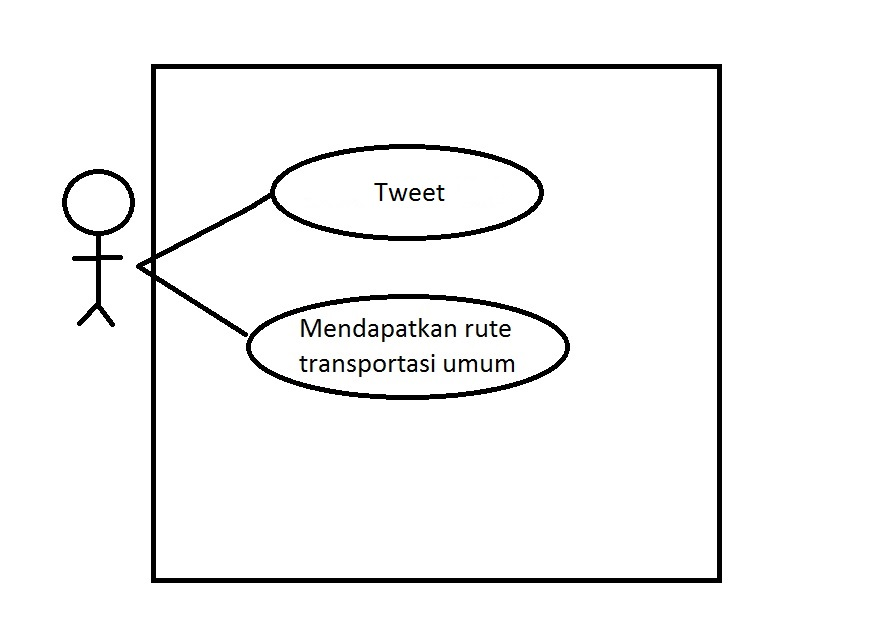
\includegraphics{Gambar/usecase.jpg}
	\caption{Use case Twitter Bot}
	\label{fig:usecase}
\end{figure}

\paragraph{Skenario \textit{Use Case}}
Skenario ini hanya memiliki satu aktor yaitu pengguna. \textit{Tweet} mencari informasi transportasi publik pada skenario ini dilakukan dengan melakukan \textit{tweet} kepada user @kiriupdate berisikan format yang sesuai untuk pencarian rute transportasi. 

\begin{table}[h]
	\begin{tabular}{|l|l|}
	\hline
	Nama           & \textit{Tweet} mencari informasi transportasi publik      											                                                                                                              \\ \hline
	Aktor          & Pengguna                                                                                                                       \\ \hline
	Deskripsi      & \begin{tabular}[c]{@{}l@{}}Melakukan \textit{Tweet}\\ (\textit{Tweet} berupa lokasi asal dan lokasi tujuan)\end{tabular}                         \\ \hline
	Kondisi Awal   & Belum menuliskan \textit{Tweet} pada kolom update                                                                                       \\ \hline
	Kondisi Akhir  & Sudah melakukan \textit{Tweet} kepada user @kiriupdate                                                                                  \\ \hline
	Skenario Utama & \begin{tabular}[c]{@{}l@{}}Pengguna melakukan \textit{Tweet} kepada \textit{user}\\ @kiriupdate dengan format yang sudah ditentukan\end{tabular} \\ \hline
	Eksepsi        & Format penulisan salah                                                                                                         \\ \hline
	\end{tabular}
	\caption{Skenario \textit{Tweet} mencari informasi transportasi }
	\label{tab:SkenarioTweetMencariInformasiTransportasi}
\end{table}

\subsection{\textit{Class Diagram}}
Untuk membuat \textit{class diagram} Twitter Bot untuk mencari jalur transportasi publik, dibutuhkan kebutuhan kelas dari skrenario. Pada skenario masukan akan terjadi hal-hal seperti dibawah ini:
\begin{enumerate}
	\item Perangkat lunak akan berjalan terus untuk menjalankan Twitter Bot.
	\item Pengguna melakukan \textit{Tweet} mencari informasi transportasi dengan cara melakukan \textit{mention} kepada \textit{user} @kiriupdate dengan format yang sesuai dengan ketentuan.
	\item Perangkat lunak menerima mention dari pengguna.
	\item Perangkat lunak akan mencari jalur transportasi umum.
	\item Melalukan \textit{reply} kepada pengguna berupa jalur transportasi publik yang harus ditempuh. 
\end{enumerate}

Berikut adalah \textit{class diagram} sederhana:
\begin{figure}[htbp]
	\centering
		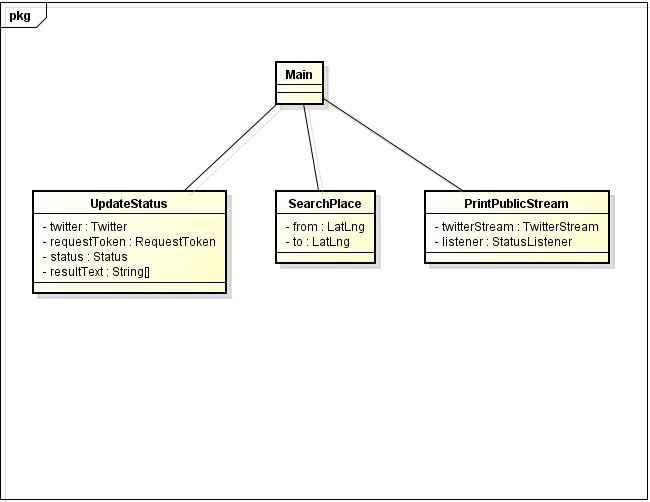
\includegraphics{Gambar/diagramClass.jpg}
	\caption{\textit{Class Diagram} Twitter Bot}
	\label{fig:classdiagram}
\end{figure}}{}
\ifdefstring{\vbaba}{1}{\chapter{Perancangan Perangkat Lunak}
\label{chap:perancangan perangkat lunak}

Pada bab ini akan dibahas mengenai perancangan aplikasi untuk membuat \textit{Twitter bot} untuk mencari jalur transportasi publik sesuai analisa yang sudah dibahas pada bab 3.

\section{Perancangan Perangkat Lunak}

\subsection{Perancangan Kelas}
Sub bab ini akan membahas tentang rancangan kelas dan \textit{method} yang akan dibuat pada perangkat lunak \textit{Twitter bot} untuk mencari jalur transportasi publik. Untuk lebih jelas mengenai kelas yang ada pada aplikasi ini, penulis menyajikan gambar kelas diagram yang dapat dilihat pada gambar ~\ref{fig:classDiagramSkripsi}

\begin{figure}[htbp]
	\centering
		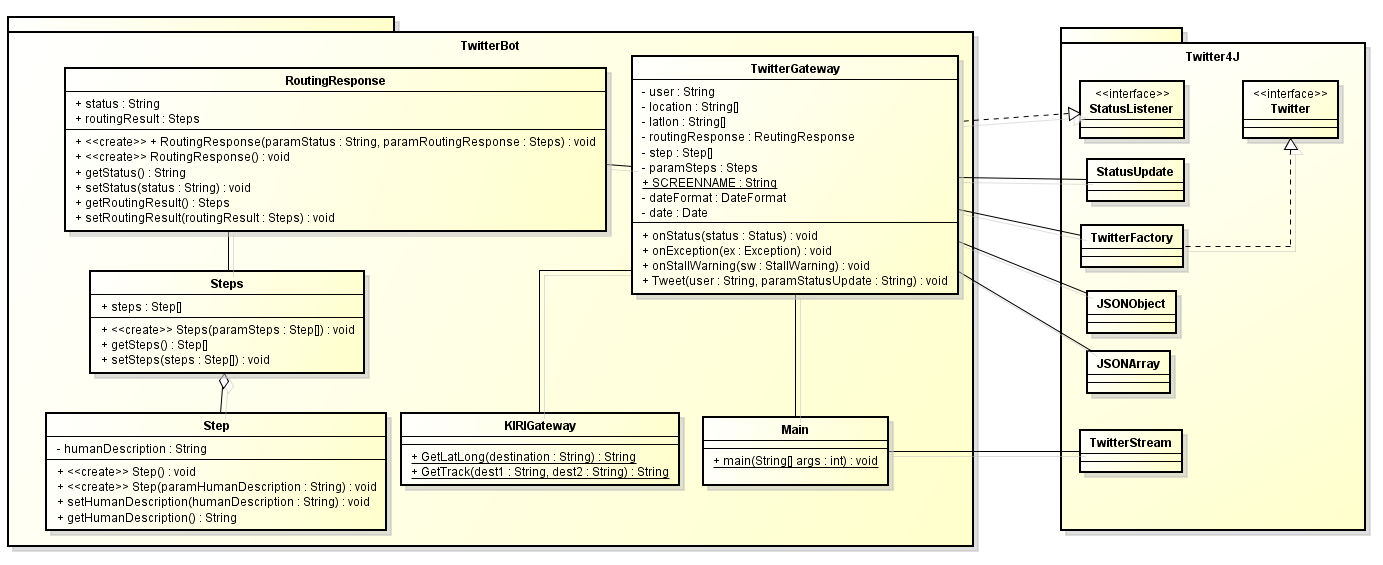
\includegraphics[width=1.00\textwidth]{C:/Skripsi/doc/DokumenSkripsi/Gambar/classDiagramSkripsi.PNG}
	\caption{Class Diagram Pembuatan \textit{Twitter bot} untuk Mencari Jalur Transportasi Publik}
	\label{fig:classDiagramSkripsi}
\end{figure}


\begin{itemize}
		\item Kelas Main, merupakan kelas yang berfungsi untuk membuat koneksi dengan Twitter ketika perangkat lunak dijalankan.
		
				\begin{itemize}
							\item Method
							
									\begin{itemize}
												\item public static void main(String[] args), merupakan method main untuk menjalankan program.
										
									\end{itemize}
				\end{itemize}
		
		\item Kelas Twitter Gateway, merupakan kelas untuk menangkap dan membalas \textit{tweet}. Kelas Twitter Gateway ini mengimplementasikan \textit{StatusListener}.
		
		
				\begin{itemize}
							\item Atribut
							
							
									\begin{itemize}
												\item String user, digunakan untuk menampung nama akun pengguna \textit{Twitter bot}.
												\item String location[], berupa \textit{array} yang digunakan untuk menampung lokasi awal dan lokasi tujuan.
												\item String latlon[], berupa \textit{array} yang digunakan untuk menampung koordinat lokasi awal dan koordinat lokasi tujuan.
												\item RoutingResponse routingResponse, merupakan atribut yang digunakan untuk menampung hasil yang diberikan oleh KIRI API.
												\item Step[] step, berupa \textit{array} yang berguna untuk menampung langkah-langkah informasi perjalanan.
												\item Steps steps, merupakan atribut yang berguna untuk menampung semua step.
									\end{itemize}
							
							\item Method
							
									\begin{itemize}
												\item public void onStatus(Status status), merupakan \textit{method} berguna yang menangkap \textit{tweet} dan memproses \textit{tweet} tersebut. Jika ada \textit{tweet} yang di-\textit{mention} kepada akun \textit{Twitter bot} dan \textit{tweet} yang diterima merupakan \textit{tweet} untuk mencari jalur transportasi publik maka \textit{tweet} tersebut akan dimasukan ke atribut yang sudah disediakan. Atribut tersebut antara lain adalah \textit{user}, lokasi awal dan lokasi tujuan. Setelah mendapatkan lokasi awal dan lokasi tujuan barulah proses pencarian dimulai dengan menggunakan \textit{method GetLatLong} dan \textit{method GetTrack} yang terdapat di kelas KIRIGateway. Hasil pencarian akan dimasukan ke dalam atribut \textit{routingResponse}, \textit{step}, dan \textit{steps}. Setelah itu akan dilakukan pemanggilan \textit{method Tweet} untuk melakukan proses \textit{reply}.
												\item public void onDeletionNotice(StatusDeletionNotice statusDeletionNotice), merupakan method overload dari kelas \textit{interface} \textit{StatusListener}.
												\item public void onTrackLimitationNotice(int numberOfLimitedStatuses), merupakan method overload dari kelas \textit{interface} \textit{StatusListener}.
												\item public void onScrubGeo(long userId, long upToStatusId), merupakan method overload dari kelas \textit{interface} \textit{StatusListener}.
												\item public void onException(Exception ex), merupakan method yang berguna untuk menangkap \textit{exception}.
												\item public void onStallWarning(StallWarning sw), merupakan method overload dari kelas \textit{interface} \textit{StatusListener}.
												\item public void Tweet(String user, String paramStatusUpdate), merupakan \textit{method} untuk melakukan \textit{reply} yang ditujukan kepada \textit{user} pengguna \textit{Twitter bot}. Twitter hanya dapat melakukan \textit{tweet} dengan batas 140 karakter, oleh karena itu method ini akan mengatasi keterbatasan \textit{tweet} tersebut dengan melakukan pembagian tweet. Method ini akan memberi tambahan waktu yang sesuai dengan server di setiap akhir \textit{tweet}, hal ini bertujuan untuk menghindari adanya duplikat tweet.
									\end{itemize}
				\end{itemize}
		
		\item Kelas KIRIGateway, merupakan kelas untuk memanggil KIRI API. Pemanggilan KIRI API ini digunakan untuk mendapatkan koordinat suatu lokasi dan mencari jalur transportasi publik.
		
		
				\begin{itemize}
							\item Method
							
							
									\begin{itemize}
												\item public static String GetLatLong(String destination), merupakan \textit{method} yang digunakan untuk mencari koordinat dari suatu lokasi. Hasil kembalian dari \textit{method} ini berupa \textit{latitude} and \textit{longitude} yang diberikan oleh KIRI API lalu diubah ke dalam bentuk \textit{String}.
												\item public static String GetTrack(String dest1, String dest2), merupakan \textit{method} yang digunakan untuk mencari jalur transportasi publik dari lokasi awal ke lokasi tujuan. Hasil kembalian dari method ini adalah langkah-langkah perjalanan dari lokasi awal ke lokasi tujuan dengan menggunakan transportasi publik.
									\end{itemize}
				\end{itemize}
		
		
		\item Kelas RoutingResult, merupakan kelas untuk menampung hasil kembalian dari KIRI API
		
		
				\begin{itemize}
							\item Atribut
					
					
									\begin{itemize}
												\item status, merupakan atribut yang digunakan untuk menyimpan status dari hasil pencarian.
												\item routingResult, merupakan atribut yang digunakan untuk menyimpan langkah-langkah perjalanan.
									\end{itemize}
					
							\item Method
					
					
									\begin{itemize}
												\item public RoutingResponse(String paramStatus, Steps paramRoutingResult), merupakan \textit{constructor} dari kelas RoutingResult.
												\item public RoutingResponse(), merupakan \textit{constructor} dari kelas RoutingResult.
												\item public String getStatus(), merupakan \textit{getter} dari atribut status.
												\item public void setStatus(String status), merupakan \textit{setter} dari atribut status.
												\item public Steps getRoutingResult(), merupakan \textit{getter} dari atribut routingResult.
												\item public void setRoutingResult(Steps routingResult), merupakan \textit{setter} dari atribut routingResult.
									\end{itemize}
				\end{itemize}
		
		\item Kelas Step, merupakan kelas untuk menampung jalur perjalanan dari lokasi awal ke lokasi tujuan dengan menggunakan transportasi publik yang diberikan oleh KIRI API.
		
		
				\begin{itemize}
							\item Atribut
					
					
									\begin{itemize}
												\item String humanDescription, merupakan atribut untuk menjelaskan cara perjalanan yang bahasanya dimengerti oleh pengguna.
									\end{itemize}
					
							\item Method
					
					
									\begin{itemize}
												\item public Step(), merupakan \textit{constructor} dari kelas Step.
												\item public Step(String paramHumanDescription), merupakan \textit{constructor} dari kelas Step.
												\item public String getHumanDescription(), merupakan \textit{getter} dari atribut humanDescription.
												\item public void setHumanDescription(String humanDescription), merupakan \textit{setter} dari atribut humanDescription.
									\end{itemize}
				\end{itemize}
		
		\item Kelas Steps, merupakan kelas untuk menampung kumpulan step.
		
		
				\begin{itemize}
							\item Atribut
					
					
									\begin{itemize}
												\item Step[] steps, merupakan atribut yang berisi \textit{array} step
									\end{itemize}
					
							\item Method
					
					
									\begin{itemize}
												\item public Steps(Step[] paramSteps), merupakan konstruktor dari kelas Steps.
												\item public Step[] getSteps(), merupakan \textit{getter} dari atribut steps.
												\item public void setSteps(Step[] steps), merupakan \textit{setter} dari atribut steps.
									\end{itemize}
				\end{itemize}
\end{itemize}




\subsection{Sequence Diagram}

Pada sub bab ini, akan dijelaskan alur program dengan menggunakan \textit{sequence diagram} pada ~\ref{fig:Sequence Diagram Final}

\begin{sidewaysfigure}[htbp]
	\centering
		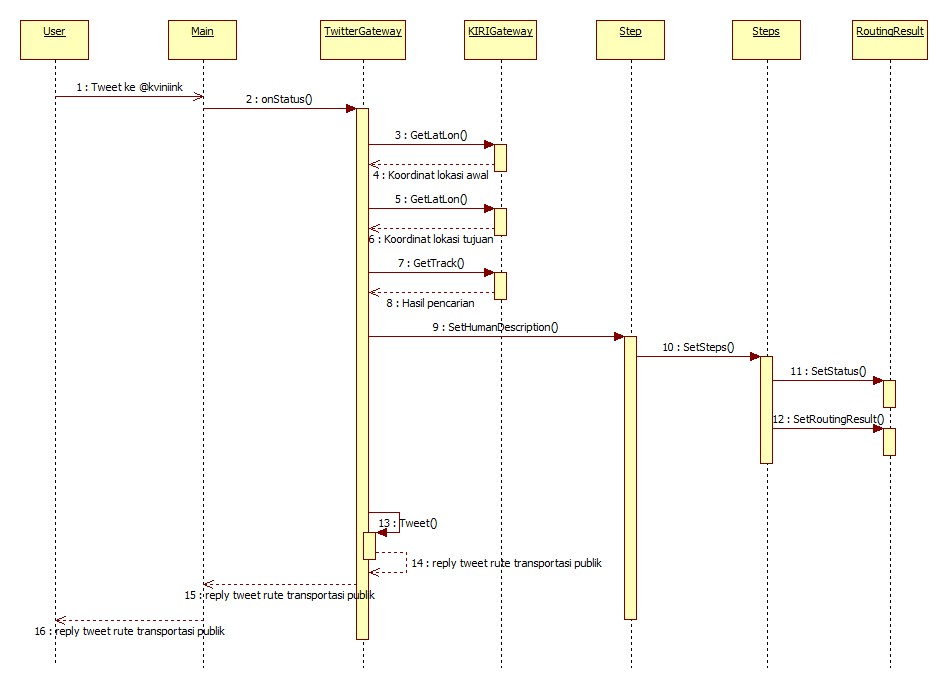
\includegraphics[width=1.00\textwidth]{C:/Skripsi/doc/DokumenSkripsi/Gambar/Sequence Diagram Final.jpg}
	\caption{Sequence Diagram \textit{Twitter bot} untuk Mencari Jalur Transportasi Publik}
	\label{fig:Sequence Diagram Final}
\end{sidewaysfigure}


Pertama, program akan melakukan \textit{streaming} pada saat kelas \textit{main} dijalankan. Kelas \textit{main} akan membuka gerbang untuk mengakses \textit{Twitter API}, dengan menggunakan \textit{Streaming} API aplikasi akan menangkap semua \textit{tweet} yang \textit{mention} kepada akun \textit{Twitter bot} @kviniink. Aplikasi akan terus melakukan \textit{streaming tweet} hingga aplikasi dinon-aktifkan.

Kelas TwitterGateway akan memproses \textit{tweet} yang di-\textit{mention} kepada akun \textit{Twitter bot} @kviniink. \textit{Method onStatus} akan melakukan pengecekan apakah \textit{tweet} tersebut merupakan \textit{tweet} untuk mencari jalur transportasi publik atau bukan. Jika benar maka nama \textit{user} pengirim, lokasi awal dan lokasi tujuan akan disimpan di atribut yang sudah disediakan lalu akan dicari koordinat dari masing-masing lokasi menggunakan KIRI API. Proses mencari koordinat ini dilakukan oleh kelas KIRIGateway.

Kelas KIRIGateway akan memanggil \textit{method GetLatLon} untuk mencari koordinat suatu lokasi. Setelah didapatkan koordinat lokasi awal dan lokasi tujuan, kelas TwitterGateway akan mengubah hasil dari \textit{method GetLatLon} yang berupa \textit{JSON} menjadi format \textit{String}. Setelah didapatkan koordinat lokasi awal dan koordinat lokasi tujuan maka hasil dari masing-masing koordinat dikembalikan kepada kelas KIRIGateway untuk dicari jalur transportasi publik dari lokasi awal menuju lokasi tujuan menggunakan \textit{method GetTrack}. Hasil dari \textit{method GetTrack} akan disimpan pada atribut \textit{step, steps}, dan \textit{routingResult}.

Setelah selesai, langkah-langkah jalur transportasi publik siap di \textit{reply} kepada pengguna. Proses \textit{reply} dilakukan oleh \textit{method tweet} yang terdapat pada kelas TwitterGateway. Tweet tersebut berisi tentang jalur transportasi publik dari lokasi awal menuju lokasi tujuan.\textit{Tweet} akan di-\textit{reply} satu per satu sesuai dengan banyaknya \textit{step} yang ada. Aplikasi akan terus melakukan proses tersebut hingga aplikasi di\textit{non-aktifkan}.

\iffalse
\subsection{Perancangan Antar Muka}
Aplikasi yang akan dibangun tidak memiliki antarmuka. Interaksi dengan pengguna dapat dilakukan melalui website atau aplikasi Twitter. Gambar ~\ref{fig:Homepage Mobile Twitter} adalah tampilan antar muka dari Twitter yang diakses melalui mobile. Dari situlah, pengguna dapat melakukan tweet untuk mencari jalur transportasi publik. Tweet dilakukan dengan cara menuliskan tweet kepada user @kviniink.

\begin{figure}[htbp]
	\centering
		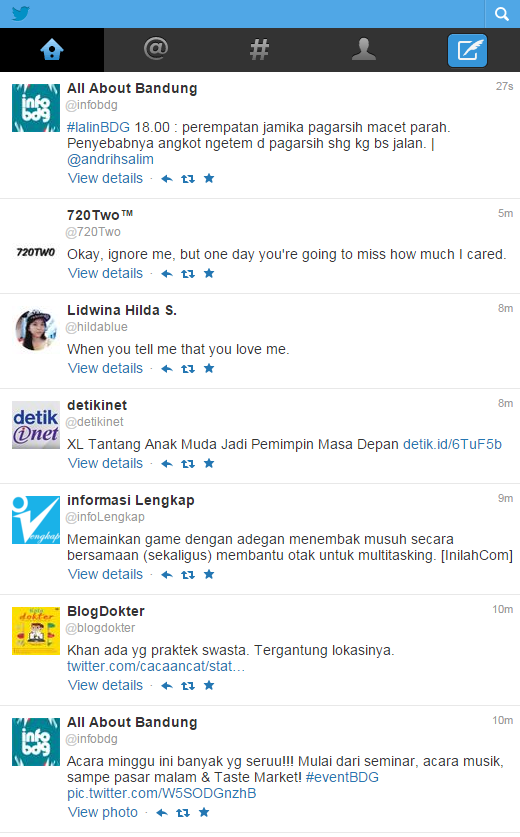
\includegraphics[width=1.00\textwidth]{C:/Skripsi/doc/DokumenSkripsi/Gambar/Homepage Mobile Twitter.PNG}
	\caption{Homepage Twitter versi mobile}
	\label{fig:Homepage Mobile Twitter}
\end{figure}

Gambar ~\ref{fig:Textbox Mobile Tweet} menunjukan menu untuk melakukan tweet. Pertama, format yang dimasukan harus benar. Format dari penulisan tweet adalah "`lokasi awal"' to "`lokasi tujuan"'. Ketika user melakukan tweet maka \textit{Twitter bot} untuk mencari jalur transportasi publik akan menangkap tweet tersebut dan akan memproses tweet tersebut, rancangan dari hasil tangkapan tweet dapat dilihat pada gambar ??. Sedangkan rancangan dari hasil pencarian dapat dilihat pada gambar ??.

\begin{figure}[hp]
	\centering
		
\includegraphics[width=1.00\textwidth]{C:/Skripsi/doc/DokumenSkripsi/Gambar/Textbox Mobile Tweet.PNG}
	\caption{Tampilan untuk melakukan tweet}
	\label{fig:Textbox Mobile Tweet}
\end{figure}
\fi



}{}
\ifdefstring{\vbaba}{1}{\chapter{Implementasi Dan Pengujian Aplikasi}
\label{chap:implementasi dan pengujian aplikasi}

Pada bab 5 akan dibahas implementasi dan pengujian aplikasi pembuatan \textit{Twitter bot} untuk mencari jalur transportasi publik.

\section{Lingkungan Pembangunan}
Lingkungan perangkat lunak dan perangkat keras yang digunakan untuk membangun dan menguji aplikasi pembuatan \textit{Twitter bot} untuk mencari jalur transportasi publik ini adalah:
\begin{itemize}
	\item Komputer
	
	
	\begin{itemize}
		\item Processor: Intel Core i7-2630QM CPU 2.00 GHz
		\item RAM: 4096MB
		\item Hardisk: 211GB
		\item VGA : NVDIA GeForce GT 540M
	\end{itemize}
	\item Sistem operasi: Windows 7 Professional
	\item Platform: NetBeans: IDE 8.0.2
	
	\item Akun \textit{Twitter bot}
	\begin{itemize}
		\item Nama akun: kviniink
		\item ConsumerKey : 3iT8duMItTTrdaU1qTHxwDIUl
		\item ConsumerSecret : YUIgJTbQT3i5tYA5RE0L38dPT9HaDhuBTifvVmKDYeOgJ7t313
		\item AccessToken : 313287708-NO5SPbreQvoOxtXUD5EcKlubIfCBNfCb6aRqYBlZ
		\item AccessTokenSecret : LVfDgtlfeht5yjBJGSgvSvtMYcFMoEdYOspYoOptcuR4i
	\end{itemize}
	
	\item Akun Twitter penguji : kviniinktest123
\end{itemize}


\section{Hasil Penggunaan Antarmuka}
Pembuatan perangkat lunak \textit{Twitter bot} untuk mencari jalur transportasi publik ini memiliki tampilan antarmuka berbasis teks yang berguna untuk melihat hasil \textit{tweet} yang diterima \textit{Twitter bot}, dan hasil \textit{tweet} yang di-\textit{reply} \textit{Twitter bot} kepada pengguna. Gambar~\ref{fig:antarmukaProgram} adalah tampilan antarmuka \textit{Twitter bot} untuk mencari jalur transportasi publik.

\begin{figure}
	\centering
		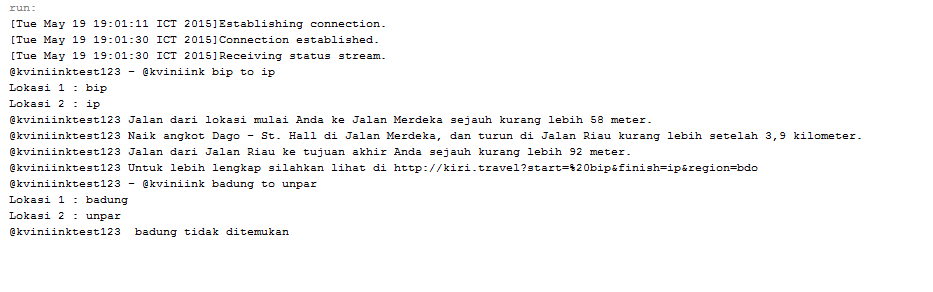
\includegraphics[width=0.75\textwidth]{C:/Skripsi/doc/DokumenSkripsi/Gambar/antarmukaProgram.PNG}
	\caption{Antarmuka Perangkat Lunak Twitter Bot Untuk Mencari Jalur Transportasi Publik}
	\label{fig:antarmukaProgram}
\end{figure}

\paragraph{Antarmuka Twitter}
Pengguna dapat mencoba perangkat lunak \textit{Twitter bot} menggunakan Twitter, baik menggunakan \textit{website} Twitter ataupun aplikasi Twitter. Oleh karena itu, tampilan antarmuka setiap pengguna akan berbeda-beda sesuai dengan \textit{device} yang digunakan pengguna. Berikut adalah contoh beberapa tampilan antarmuka yang diberikan oleh Twitter:

\begin{itemize}
	\item Antarmuka Twitter yang diakses melalui aplikasi Twitter di Android dapat dilihat pada Gambar~\ref{fig:TwitterAndroid}
			
			\begin{figure}[htbp]
				\centering
					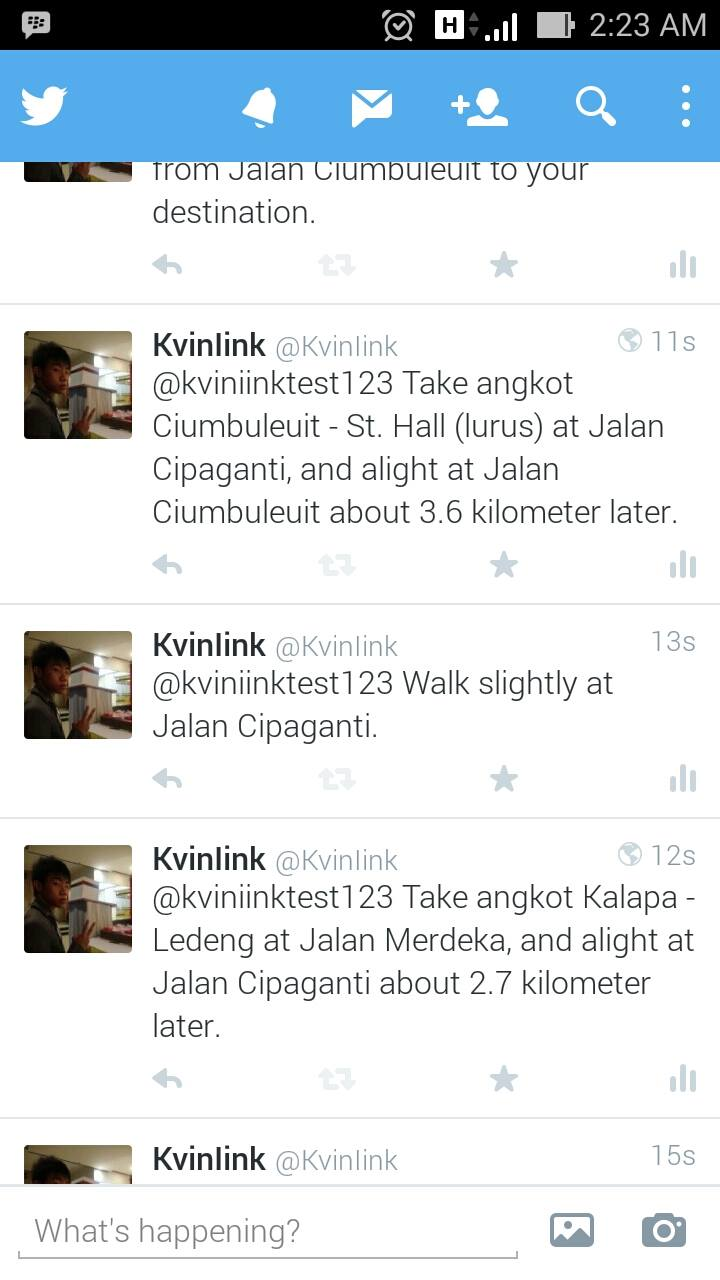
\includegraphics[width=0.5\textwidth]{C:/Skripsi/doc/DokumenSkripsi/Gambar/TwitterAndroid1.jpg}
				\caption{Antarmuka Twitter yang diakses melalui aplikasi Twitter di Android}
				\label{fig:TwitterAndroid}
			\end{figure}
			
	\item Antarmuka Twitter yang diakses melalui aplikasi Twitter di iOS dapat dilihat pada Gambar~\ref{fig:TwitteriOS}
	
	
	\begin{figure}[htbp]
		\centering
			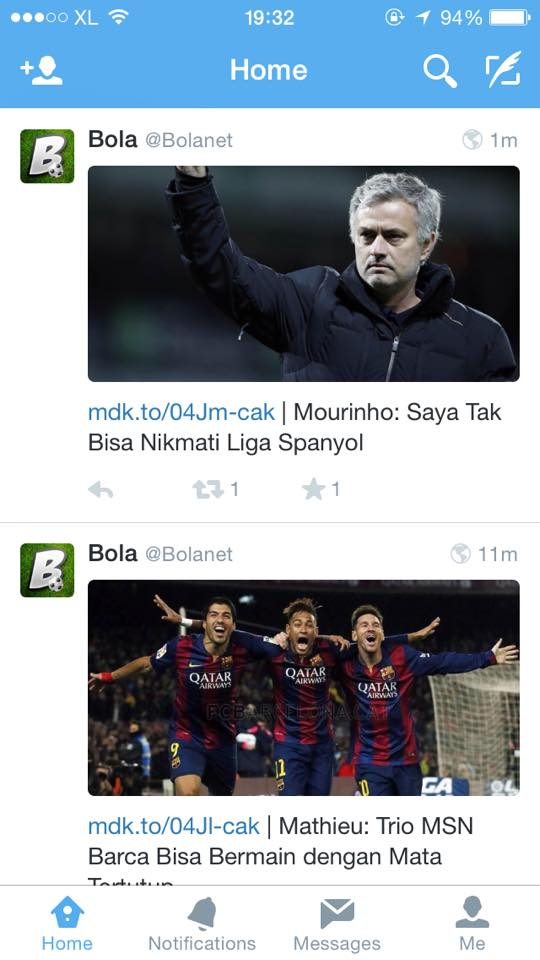
\includegraphics[width=0.5\textwidth]{C:/Skripsi/doc/DokumenSkripsi/Gambar/TwitteriOS.jpg}
		\caption{Antarmuka Twitter yang diakses melalui aplikasi Twitter di iOS}
		\label{fig:TwitteriOS}
	\end{figure}
	
	\item Antarmuka Twitter yang diakses melalui aplikasi Twitter di Windows Phone dapat dilihat pada Gambar~\ref{fig:TwitterWP}
	
	
	\begin{figure}[htbp]
		\centering
			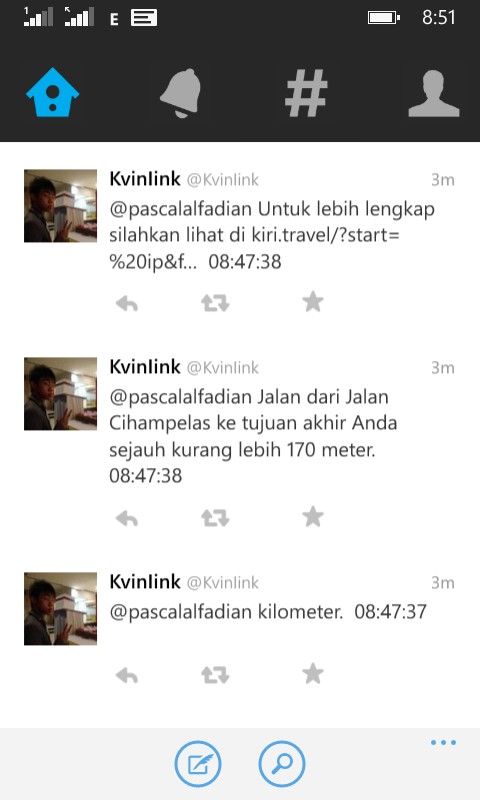
\includegraphics[width=0.5\textwidth]{C:/Skripsi/doc/DokumenSkripsi/Gambar/TwitterWP.jpg}
		\caption{Antarmuka Twitter yang diakses melalui aplikasi Twitter di Windows Phone}
		\label{fig:TwitterWP}
	\end{figure}
	
	
	\item Antarmuka Twitter yang diakses melalui aplikasi Twitter di Website Twitter dapat dilihat pada Gambar~\ref{fig:homePageTwitter}

	
	\begin{figure}[htbp]
		\centering
			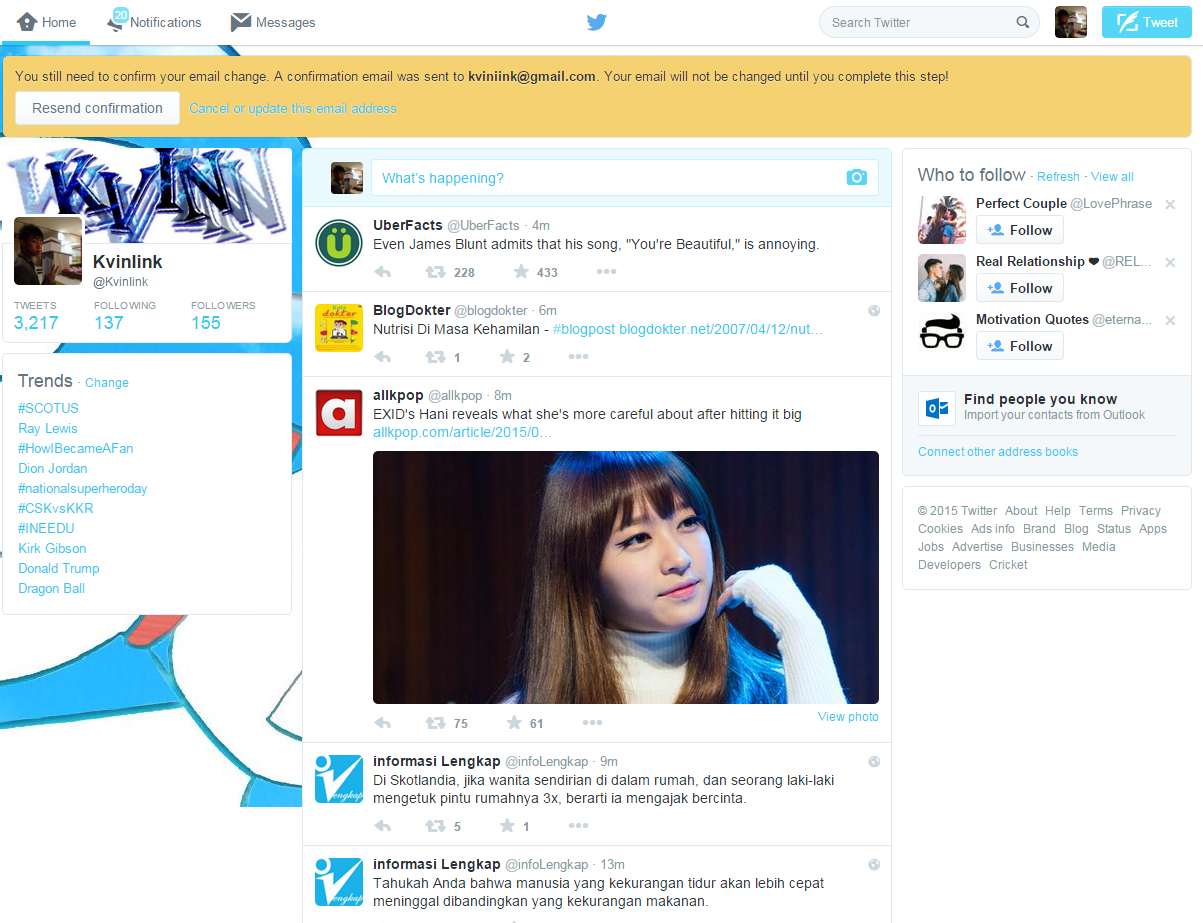
\includegraphics[width=0.75\textwidth]{C:/Skripsi/doc/DokumenSkripsi/Gambar/homePageTwitter.PNG}
		\caption{Antarmuka Twitter yang diakses melalui aplikasi Twitter di Website Twitter}
		\label{fig:homePageTwitter}
	\end{figure}
	
\end{itemize}

\iffalse
Tampilan \textit{home page} Twitter dapat dilihat pada Gambar~\ref{fig:Homepage Mobile Twitter}. Disini peneliti menggunakan website Twitter versi mobile agar lebih mudah dilihat karena tampilan website Twitter versi mobile lebih sederhana dibandingkan website Twitter versi desktop. Setelah itu user akan menekan tombol \textit{tweet} pada pojok kanan atas dan akan memberikan tampilan seperti pada Gambar~\ref{fig:Textbox Mobile Tweet}. Dari situ user dapat melakukan \textit{tweet} kepada \textit{Twitter Bot} untuk mencari jalur transportasi publik.
\begin{figure}[htbp]
	\centering
		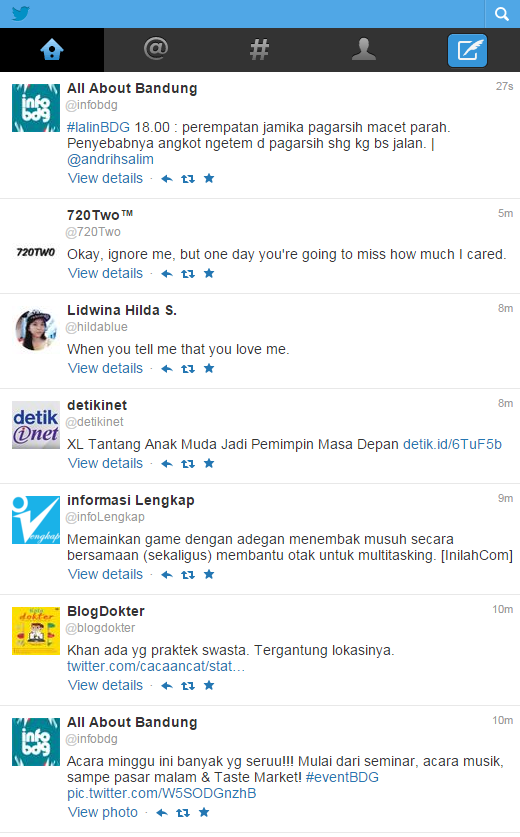
\includegraphics[width=1.00\textwidth]{C:/Skripsi/doc/DokumenSkripsi/Gambar/Homepage Mobile Twitter.PNG}
	\caption{Homepage Twitter versi mobile}
	\label{fig:Homepage Mobile Twitter}
\end{figure}


\begin{figure}[htbp]
	\centering
		
\includegraphics[width=1.00\textwidth]{C:/Skripsi/doc/DokumenSkripsi/Gambar/Textbox Mobile Tweet.PNG}
	\caption{Tampilan untuk melakukan \textit{tweet}}
	\label{fig:Textbox Mobile Tweet}
\end{figure}

Setelah ada \textit{mention} yang ditujukan kepada \textit{Twitter Bot}, aplikasi akan menangkap \textit{tweet} tersebut dan ditampilkan dalam bentuk pesan \textit{tweet} yang diterima oleh aplikasi. Hasil \textit{tweet} yang diterima aplikasi dapat dilihat pada Gambar~\ref{fig:HasilTangkapanTweetBerbasisTeks}. Setelah itu \textit{tweet} akan diperiksa oleh aplikasi apakah \textit{tweet} tersebut bertujuan untuk mencari jalur transportasi publik atau tidak. Jika benar, maka aplikasi akan melakukan proses pencarian jalur transportasi publik dan melakukan \textit{reply} atau balasan kepada pengguna. \textit{Reply tweet} tersebut berisikan jalur transportasi publik yang harus ditempuh kepada \textit{user}. Selain melakukan \textit{reply}, aplikasi juga menampilkan \textit{tweet} tersebut yang dapat dilihat pada Gambar~\ref{fig:HasilTweetBerbasisTeks}.

\begin{figure}
	\centering
		
\includegraphics{C:/Skripsi/doc/DokumenSkripsi/Gambar/HasilTangkapanTweetBerbasisTeks.PNG}
	\caption{Hasil streaming \textit{tweet}}
	\label{fig:HasilTangkapanTweetBerbasisTeks}
\end{figure}

\begin{figure}
	\centering
		
\includegraphics{C:/Skripsi/doc/DokumenSkripsi/Gambar/HasilTweetBerbasisTeks.PNG}
	\caption{Hasil balasan \textit{tweet} kepada user}
	\label{fig:HasilTweetBerbasisTeks}
\end{figure}
\fi

\newpage
\section{Pengujian}
Pada sub-bab ini akan dibahas mengenai hasil pengujian yang telah dilakukan terhadap perangkat lunak yang dibangun oleh penulis. Pengujian terdiri dari dua bagian, yaitu pengujian fungsional dan pengujian eksperimental. Pengujian fungsional bertujuan untuk memastikan semua fungsi aplikasi berjalan sesuai harapan. Sementara pengujian eksperimental bertujuan untuk mengetahui keberhasilan proses kerja dari aplikasi yang dibangun.

\subsection{Pengujian Fungsional}
Pengujian fungsional dilakukan pada fungsionalitas yang tersedia pada aplikasi yang dibangun. Pengujian ini dilakukan untuk mengetahui kesesuaian reaksi nyata dengan reaksi yang diharapkan dari aplikasi yang dibangun. Hasil pengujian ditunjukan pada tabel ~\ref{tab:TabelHasilPengujianFungsionalitasPadaAplikasiTwitterBotUntukMencariJalurTransportasiPublik}.

\begin{table}[h]
	\caption{Tabel Hasil pengujian fungsionalitas pada Aplikasi \textit{Twitter bot} untuk mencari jalur transportasi publik}
	\label{tab:TabelHasilPengujianFungsionalitasPadaAplikasiTwitterBotUntukMencariJalurTransportasiPublik}
		\begin{tabular}{|p{0.5cm}|p{3cm}|p{5cm}|p{5cm}|}
			\hline
				No & Pengujian & Reaksi yang Diharapkan & Reaksi Aplikasi  \\ \hline
				1 & Melakukan otentikasi terhadap akun \textit{Twitter Bot} & Otentikasi berhasil dilakukan antara Twitter dengan akun \textit{Twitter Bot}. Otentikasi dilakukan dengan melakukan pemeriksaan terhadap \textit{ConsumerKey}, \textit{CustomerSecret}, \textit{AccessToken}, dan \textit{AccessTokenSecret} &  \textit{ConsumerKey}, \textit{CustomerSecret}, \textit{AccessToken}, dan \textit{AccessTokenSecret} yang diberikan Twitter berhasil diotentikasi oleh aplikasi \\ \hline
				2 & Melakukan \textit{streaming tweet} & Menangkap semua \textit{tweet} yang di\textit{mention} kepada akun @kviniink & Setiap \textit{tweet} yang di\textit{mention} kepada akun \textit{Twitter bot} @kviniink dapat diterima secara \textit{realtime}\\ \hline
				3 & Membaca \textit{tweet} yang ditangkap & Melakukan pemeriksaan terhadap \textit{tweet} yang ditangkap, apakah \textit{tweet} tersebut merupakan \textit{tweet} untuk mencari transportasi publik atau bukan & Perangkat lunak dapat membedakan \textit{tweet} untuk mencari jalur transportasi publik dengan \textit{tweet} yang bukan bertujuan untuk mencari jalur transportasi publik. Selain itu Perangkat lunak dapat menangkap \textit{tweet} untuk bantuan pancarian.  \\ \hline
				4 & Melakukan pencarian koordinat suatu lokasi menggunakan KIRI API & Mendapatkan hasil koordinat \textit{latitude} dan \textit{longitude} dari lokasi yang dicari & Perangkat lunak mendapatkan koordinat \textit{latitude} dan \textit{longitude} dari lokasi yang dicari  \\ \hline
				5 & Melakukan pencarian jalur transportasi publik menggunakan KIRI API & Mendapatkan jalur-jalur transportasi publik yang harus ditempuh dari lokasi awal menuju lokasi tujuan &  Perangkat lunak mendapatkan jalur-jalur transportasi publik yang harus ditempuh dari lokasi awal menuju lokasi tujuan \\ \hline
				6 & Melakukan \textit{tweet} balasan & Membalas \textit{tweet} dengan memberikan hasil pencarian jalur transportasi publik dengan format yang sudah ditentukan &  Akun \textit{Twitter bot} @kviniink melakukan \textit{reply} kepada akun penguji @kviniinktest123, \textit{reply} tersebut berisikan jalur transportasi publik yang harus ditempuh dari lokasi awal menuju lokasi tujuan. \textit{Reply} sudah dapat dipecah-pecah jika \textit{tweet} melebihi 140 karakter.\\ \hline
		\end{tabular}
\end{table}

\subsection{Pengujian Eksperimental}
Pada sub bab ini akan dilakukan pengujian terhadap \textit{Twitter bot} untuk mencari jalur transportasi publik. Peneliti meminta kepada beberapa orang untuk melakukan pencarian jalur transportasi publik kepada \textit{Twitter bot} untuk mencari jalur transportasi publik. Selain itu juga peneliti mencoba melakukan \textit{tweet} pencarian melalui akun @kviniinktest123.

\begin{enumerate}
	\item Pengujian 1
	
	Pada pengujian satu, peneliti mencoba untuk mencari jalur transportasi publik untuk lokasi yang umum dikunjungi yaitu \textit{mall}. Pencarian dilakukan dengan lokasi awal yaitu BIP (Bandung Indah Plaza) menuju lokasi tujuan yaitu IP (Istana Plaza). Akun penguji @kviniinktest123 melakukan \textit{mention} kepada akun \textit{Twitter bot} @kviniink123 yang dapat dilihat pada Gambar~\ref{fig:Tweet1}.
	
	\begin{figure}
		\centering
			
\includegraphics[width=0.75\textwidth]{C:/Skripsi/doc/DokumenSkripsi/Gambar/Tweet1.PNG}
		\caption{Tweet dari BIP menuju IP}
		\label{fig:Tweet1}
	\end{figure}
	
	Setelah proses \textit{tweet} dilakukan, \textit{Twitter bot} akan menangkap \textit{tweet} tersebut dan memprosesnya. Setelah proses pencarian selesai dilakukan, akun \textit{Twitter bot} @kviniink melakukan \textit{reply} kepada akun @kviniinktest123 yang dapat dilihat pada Gambar~\ref{fig:HasilTweet1}. 
	
		
	\begin{figure}
		\centering
			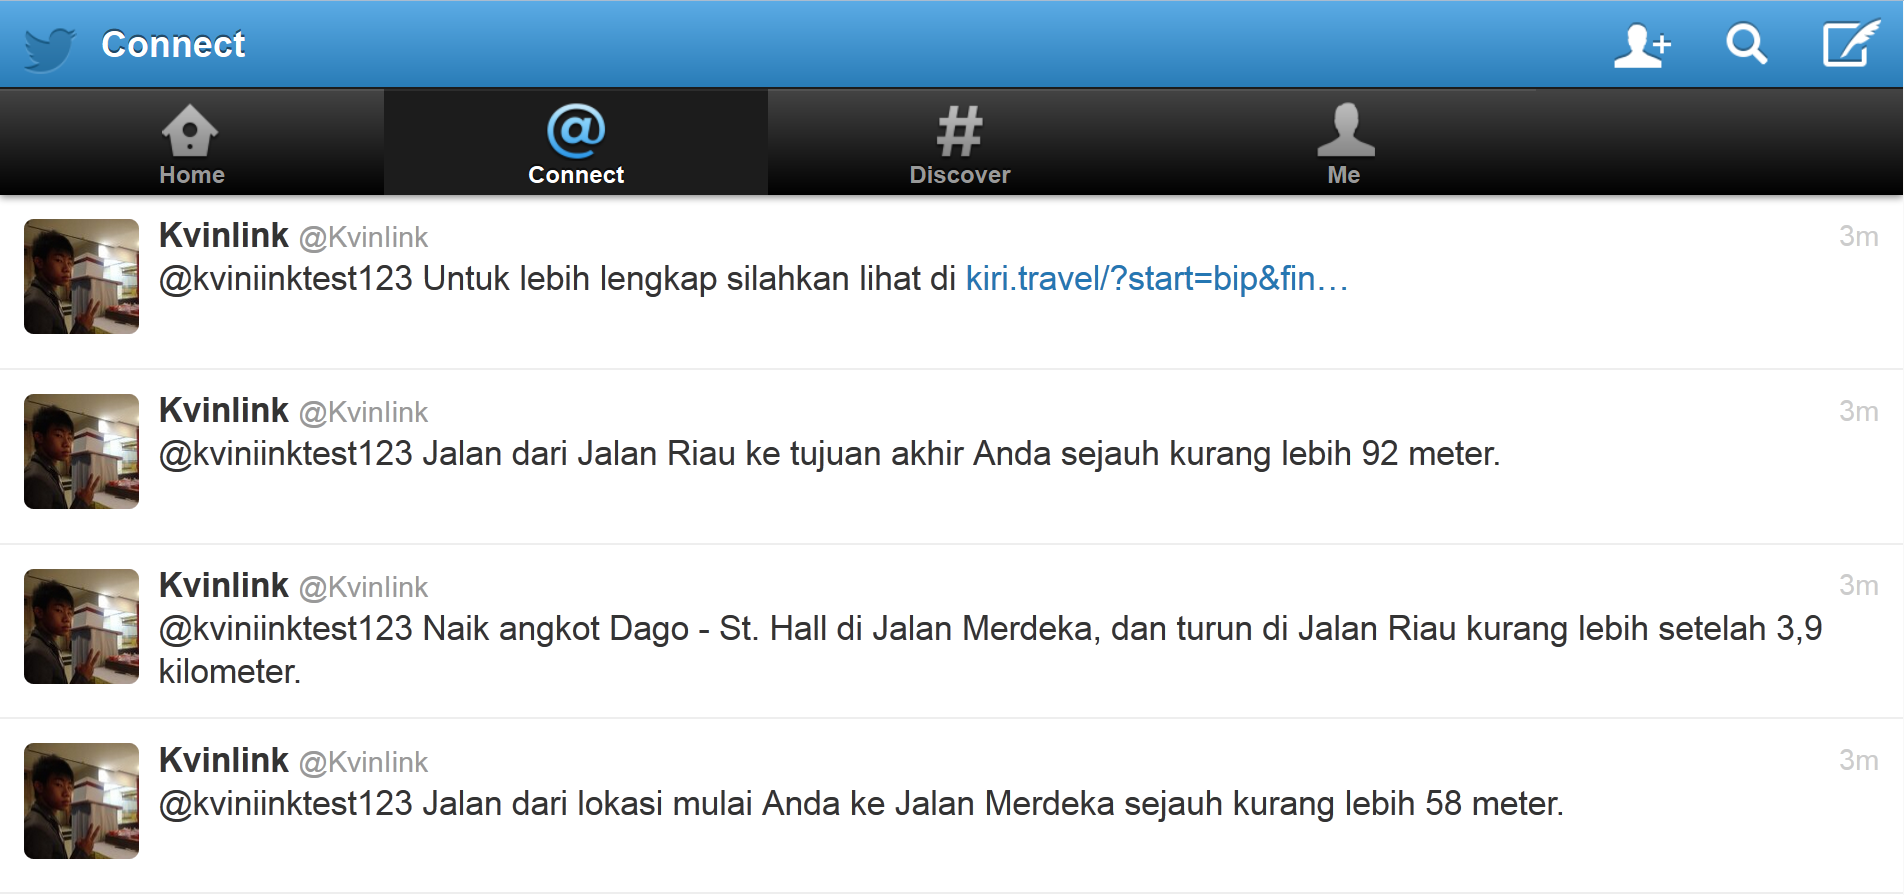
\includegraphics[width=0.75\textwidth]{C:/Skripsi/doc/DokumenSkripsi/Gambar/HasilTweet1.PNG}
		\caption{Hasil Pencarian Rute Transportasi Publik dari BIP menuju IP}
		\label{fig:HasilTweet1}
	\end{figure}
	
	Pencarian kedua dilakukan dengan lokasi awal yaitu BIP (Bandung Indah Plaza) dan lokasi tujuan yaitu PVJ (Paris van Java). Dapat dilihat pada Gambar~\ref{fig:Tweet2}, akun @kviniinktest123 melakukan \textit{tweet} pencarian jalur transportasi publik yang di-\textit{mention} kepada akun \textit{Twitter bot} @kviniink dengan lokasi awal yaitu BIP dan lokasi tujuan yaitu PVJ.
	
	\begin{figure}
		\centering
			
\includegraphics[width=0.75\textwidth]{C:/Skripsi/doc/DokumenSkripsi/Gambar/Tweet2.PNG}
		\caption{\textit{Tweet} dari BIP menuju PVJ}
		\label{fig:Tweet2}
	\end{figure}
	
	Setelah itu \textit{tweet} tersebut diproses oleh aplikasi untuk dicari jalur transportasi publiknya, lalu akun \textit{Twitter bot} @kviniink melakukan \textit{reply} kepada akun @kviniinktest123. \textit{Reply tweet} tersebut merupakan jalur transportasi publik yang harus ditempuh, \textit{reply tweet} tersebut dapat dilihat pada Gambar~\ref{fig:HasilTweet2}.
	
	
	\begin{figure}
		\centering
			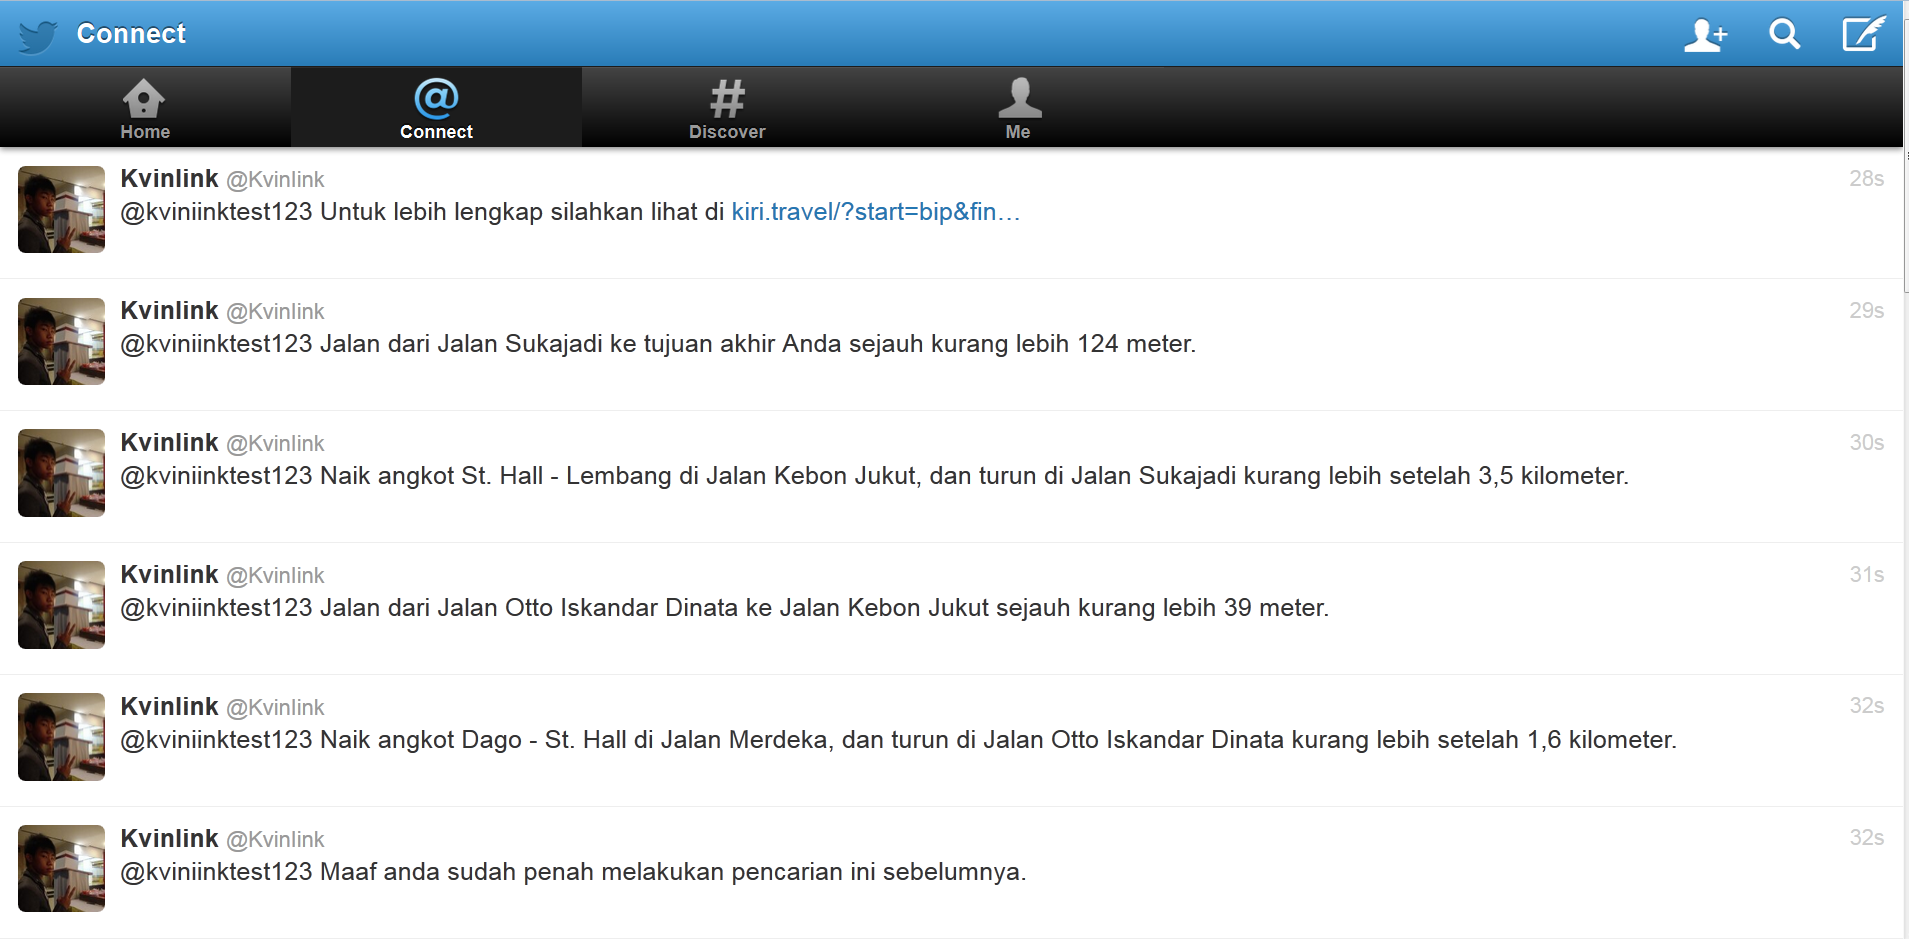
\includegraphics[width=0.75\textwidth]{C:/Skripsi/doc/DokumenSkripsi/Gambar/HasilTweet2.PNG}
		\caption{Hasil Pencarian Rute Transportasi Publik dari BIP menuju PVJ}
		\label{fig:HasilTweet2}
	\end{figure}
	
	Pada pencarian kedua dapat dilihat pada \textit{tweet} pertama terjadi ketidak sesuaian hasil dari KIRI API dengan hasil \textit{tweet}.
	Peneliti lalu melakukan pencarian melalui \textit{website} KIRI yaitu \url{http://kiri.travel}. Pencarian pertama pada \textit{website} KIRI dilakukan dengan lokasi awal yaitu BIP dan lokasi tujuan yaitu IP. Hasil pencarian pada \textit{website} KIRI dapat dilihat pada Gambar~\ref{fig:HasilKiri1}.
	
	
	\begin{figure}
		\centering
			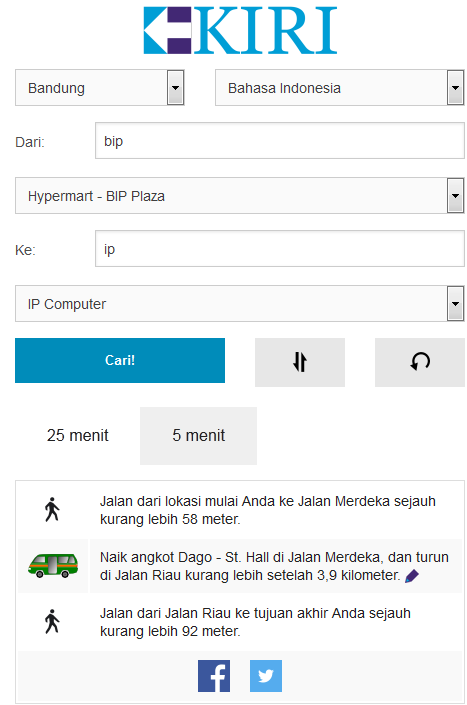
\includegraphics[width=0.5\textwidth]{C:/Skripsi/doc/DokumenSkripsi/Gambar/HasilKiri1.PNG}
		\caption{Hasil Pencarian Jalur Transportasi Publik dari BIP menuju IP Melalui Website KIRI}
		\label{fig:HasilKiri1}
	\end{figure}
	
	Lalu pencarian kedua pada \textit{website} KIRI dilakukan dengan lokasi awal yaitu BIP dan lokasi tujuan yaitu PVJ. Hasil pencarian KIRI dari BIP menuju PVJ dapat dilihat pada Gambar~\ref{fig:HasilKiri2}. Setelah dilihat dari hasil keduanya, \textit{Twitter bot} melakukan \textit{duplicate tweet} pada \textit{tweet} pertama dalam pencarian ke dua yang dilakukan oleh akun @kviniink123. \textit{Duplicate tweet} adalah \textit{tweet} yang dinyatakan dinyatakan identik oleh Twitter dalam jangka waktu tertentu. \textit{Duplicate tweet} tidak diperbolehkan oleh Twitter. Oleh karena itu, untuk menghindari adanya \textit{duplicate tweet}, penulis menambahkan waktu untuk jam, menit, dan detik di setiap \textit{tweet} yang dilakukan oleh \textit{Twitter bot} agar membuat setiap \textit{tweet} tersebut bersifat unik.
	
	\begin{figure}
		\centering
			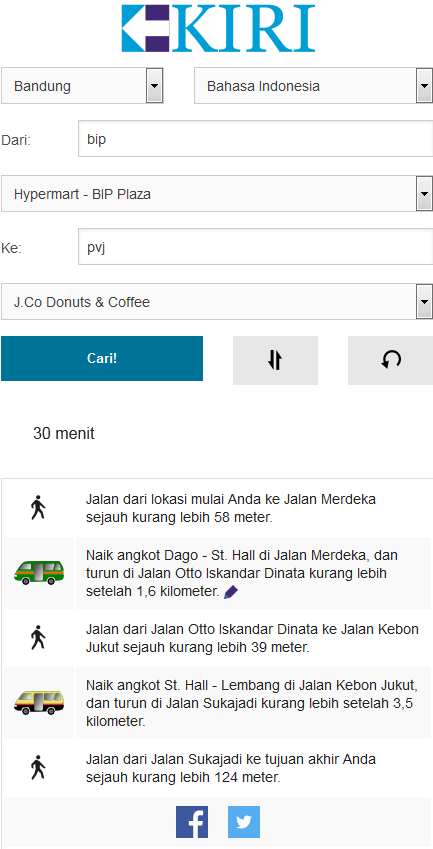
\includegraphics[width=0.5\textwidth]{C:/Skripsi/doc/DokumenSkripsi/Gambar/HasilKiri2.PNG}
		\caption{Hasil Pencarian Jalur Transportasi Publik dari BIP menuju PVJ Melalui Website KIRI}
		\label{fig:HasilKiri2}
	\end{figure}
	\clearpage
	
	\item Pengujian 1.1
	
	Pada pengujian satu, peneliti mencoba untuk mencari jalur transportasi publik untuk lokasi yang umum dikunjungi yaitu \textit{mall}. Pencarian dilakukan dengan lokasi awal yaitu PVJ (Paris Van Java) menuju lokasi tujuan yaitu BIP (Bandung Indah Plaza). Akun penguji @kviniinktest123 melakukan \textit{mention} kepada akun \textit{Twitter bot} @kviniink123 yang dapat dilihat pada Gambar~\ref{fig:Tweet1_1}.
	
	\begin{figure}
		\centering
			
\includegraphics[width=0.75\textwidth]{C:/Skripsi/doc/DokumenSkripsi/Gambar/Tweet1_1.PNG}
		\caption{Tweet dari PVJ menuju BIP}
		\label{fig:Tweet1_1}
	\end{figure}
	
	Setelah proses \textit{tweet} dilakukan, \textit{Twitter bot} akan menangkap \textit{tweet} tersebut dan memprosesnya. Setelah proses pencarian selesai dilakukan, akun \textit{Twitter bot} @kviniink melakukan \textit{reply} kepada akun @kviniinktest123 yang dapat dilihat pada Gambar~\ref{fig:HasilTweet1_1}. 
	
		
	\begin{figure}
		\centering
			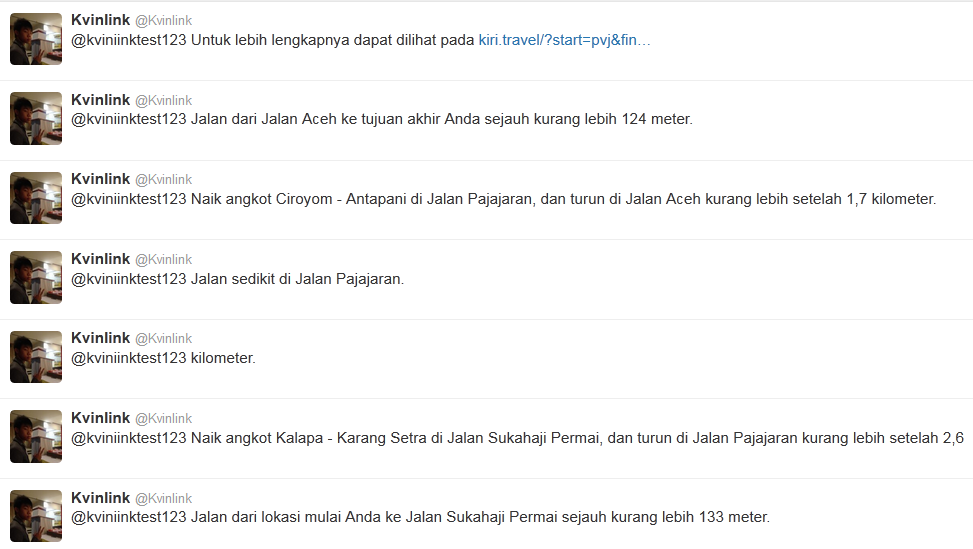
\includegraphics[width=0.75\textwidth]{C:/Skripsi/doc/DokumenSkripsi/Gambar/HasilTweet1_1.PNG}
		\caption{Hasil Pencarian Rute Transportasi Publik dari BIP menuju IP}
		\label{fig:HasilTweet1_1}
	\end{figure}
	
	Pencarian kedua dilakukan dengan lokasi awal yaitu PVJ(Paris Van Java) dan lokasi tujuan yaitu Museum KAA(Konferensi Asia Afrika). Dapat dilihat pada Gambar~\ref{fig:Tweet2_2}, akun @kviniinktest123 melakukan \textit{tweet} pencarian jalur transportasi publik yang di-\textit{mention} kepada akun \textit{Twitter bot} @kviniink dengan lokasi awal yaitu PVJ dan lokasi tujuan yaitu Museum KAA.
	
	\begin{figure}
		\centering
			
\includegraphics[width=0.75\textwidth]{C:/Skripsi/doc/DokumenSkripsi/Gambar/Tweet2_2.PNG}
		\caption{\textit{Tweet} dari PVJ menuju Museum KAA}
		\label{fig:Tweet2_2}
	\end{figure}
	
	Setelah itu \textit{tweet} tersebut diproses oleh aplikasi untuk dicari jalur transportasi publiknya, lalu akun \textit{Twitter bot} @kviniink melakukan \textit{reply} kepada akun @kviniinktest123. \textit{Reply tweet} tersebut merupakan jalur transportasi publik yang harus ditempuh, \textit{reply tweet} tersebut dapat dilihat pada Gambar~\ref{fig:HasilTweet2_2}.
	
	
	\begin{figure}
		\centering
			
\includegraphics[width=0.75\textwidth]{C:/Skripsi/doc/DokumenSkripsi/Gambar/HasilTweet2_2.PNG}
		\caption{Hasil Pencarian Rute Transportasi Publik dari PVJ menuju Museum KAA}
		\label{fig:HasilTweet2_2}
	\end{figure}
	
	Pada pencarian kedua dapat dilihat pada \textit{tweet} pertama terjadi ketidak sesuaian hasil dari KIRI API dengan hasil \textit{tweet}.
	Peneliti lalu melakukan pencarian melalui \textit{website} KIRI yaitu \url{http://kiri.travel}. Pencarian pertama pada \textit{website} KIRI dilakukan dengan lokasi awal yaitu PVJ dan lokasi tujuan yaitu BIP. Hasil pencarian pada \textit{website} KIRI dapat dilihat pada Gambar~\ref{fig:HasilKiri1}.
	
	
	\begin{figure}
		\centering
			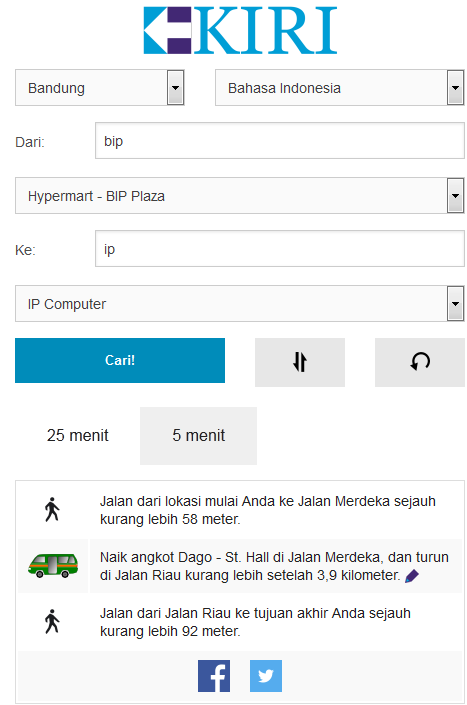
\includegraphics[width=0.5\textwidth]{C:/Skripsi/doc/DokumenSkripsi/Gambar/HasilKiri1.PNG}
		\caption{Hasil Pencarian Jalur Transportasi Publik dari BIP menuju IP Melalui Website KIRI}
		\label{fig:HasilKiri1}
	\end{figure}
	
	Lalu pencarian kedua pada \textit{website} KIRI dilakukan dengan lokasi awal yaitu PVJ dan lokasi tujuan yaitu Museum KAA. Hasil pencarian KIRI dari PVJ menuju Museum KAA dapat dilihat pada Gambar~\ref{fig:HasilKiri2}. Setelah dilihat dari hasil keduanya, \textit{Twitter bot} melakukan \textit{duplicate tweet} pada \textit{tweet} pertama dalam pencarian ke dua yang dilakukan oleh akun @kviniink123. \textit{Duplicate tweet} adalah \textit{tweet} yang dinyatakan dinyatakan identik oleh Twitter dalam jangka waktu tertentu. \textit{Duplicate tweet} tidak diperbolehkan oleh Twitter. Oleh karena itu, untuk menghindari adanya \textit{duplicate tweet}, penulis menambahkan waktu untuk jam, menit, dan detik di setiap \textit{tweet} yang dilakukan oleh \textit{Twitter bot} agar membuat setiap \textit{tweet} tersebut bersifat unik.
	
	\begin{figure}
		\centering
			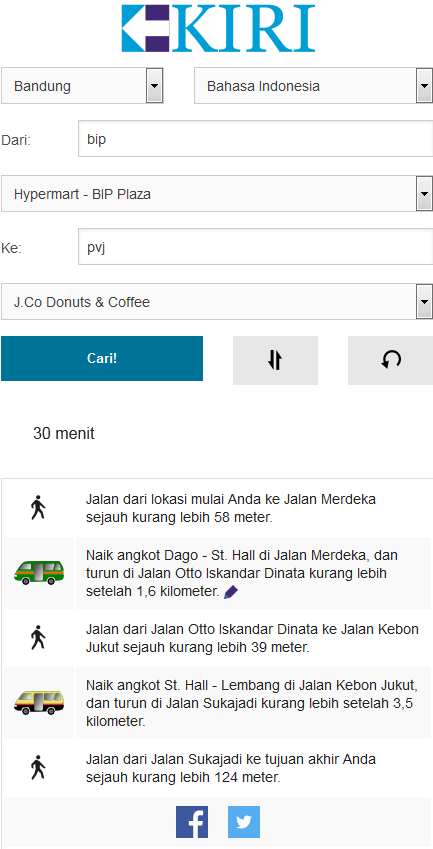
\includegraphics[width=0.5\textwidth]{C:/Skripsi/doc/DokumenSkripsi/Gambar/HasilKiri2.PNG}
		\caption{Hasil Pencarian Jalur Transportasi Publik dari BIP menuju PVJ Melalui Website KIRI}
		\label{fig:HasilKiri2}
	\end{figure}
	\clearpage
	
	\item Pengujian 2
	
	Pada pengujian dua, penulis melakukan pengujian dengan cara menjalankan aplikasi selama 24 jam. Selain itu penulis juga melakukan pengujian dengan cara meminta bantuan kepada beberapa responden untuk melakukan \textit{tweet} pencarian jalur transportasi publik. Pengujian ini dilakukan untung mengetahui apakah aplikasi \textit{Twitter bot} berjalan dengan baik atau tidak. Dari hasil yang didapatkan \textit{Twitter bot} dapat memberi pesan bahwa suatu lokasi pencarian tidak ditemukan. Pesan pemberitahuan yang dapat dilihat pada Gambar~\ref{fig:HasilFinal1}. Selain itu juga \textit{Twitter bot} dapat memberi pesan juga lokasi awal dan lokasi tujuan merupakan lokasi yang sama. Pesan pemberitahuan dapat dilihat pada Gambar~\ref{fig:HasilTweetSama}.
	Pada Gambar~\ref{fig:HasilFinal1} dapat dilihat bahwa akun @cla\_amour mencari lokasi tki dan kopo tetapi lokasi pencarian tidak ditemukan. Akun @cla\_amour juga mencari jalur transportasi publik yang lokasinya ditemukan tetapi tidak ada rute transportasi publiknya. Hasil \textit{reply Twitter bot} yang dilakukan oleh akun @cla\_amour dapat dilihat pada salah satu \textit{reply} yang terdapat pada Gambar~\ref{fig:HasilFinal1}.
	
	Selain itu \textit{Twitter bot} tidak akan mendapatkan \textit{error} ketika akun \textit{Twitter Bot} @kviniink mendapat banyak \textit{mention} dalam satu \textit{tweet} seperti pada Gambar~\ref{fig:testTweet}, jika format penulisan benar maka \textit{Twitter bot} akan tetap mencari jalur transportasi publiknya yang dapat dilihat pada Gambar~\ref{fig:hasilTestTweet}. 
	Gambar~\ref{fig:HasilFinal1}, Gambar~\ref{fig:HasilFinal2}, dan Gambar~\ref{fig:HasilFinal3} merupakan beberapa hasil \textit{reply} dari \textit{Twitter bot}.
	
	\newpage
	\begin{figure}
		\centering
			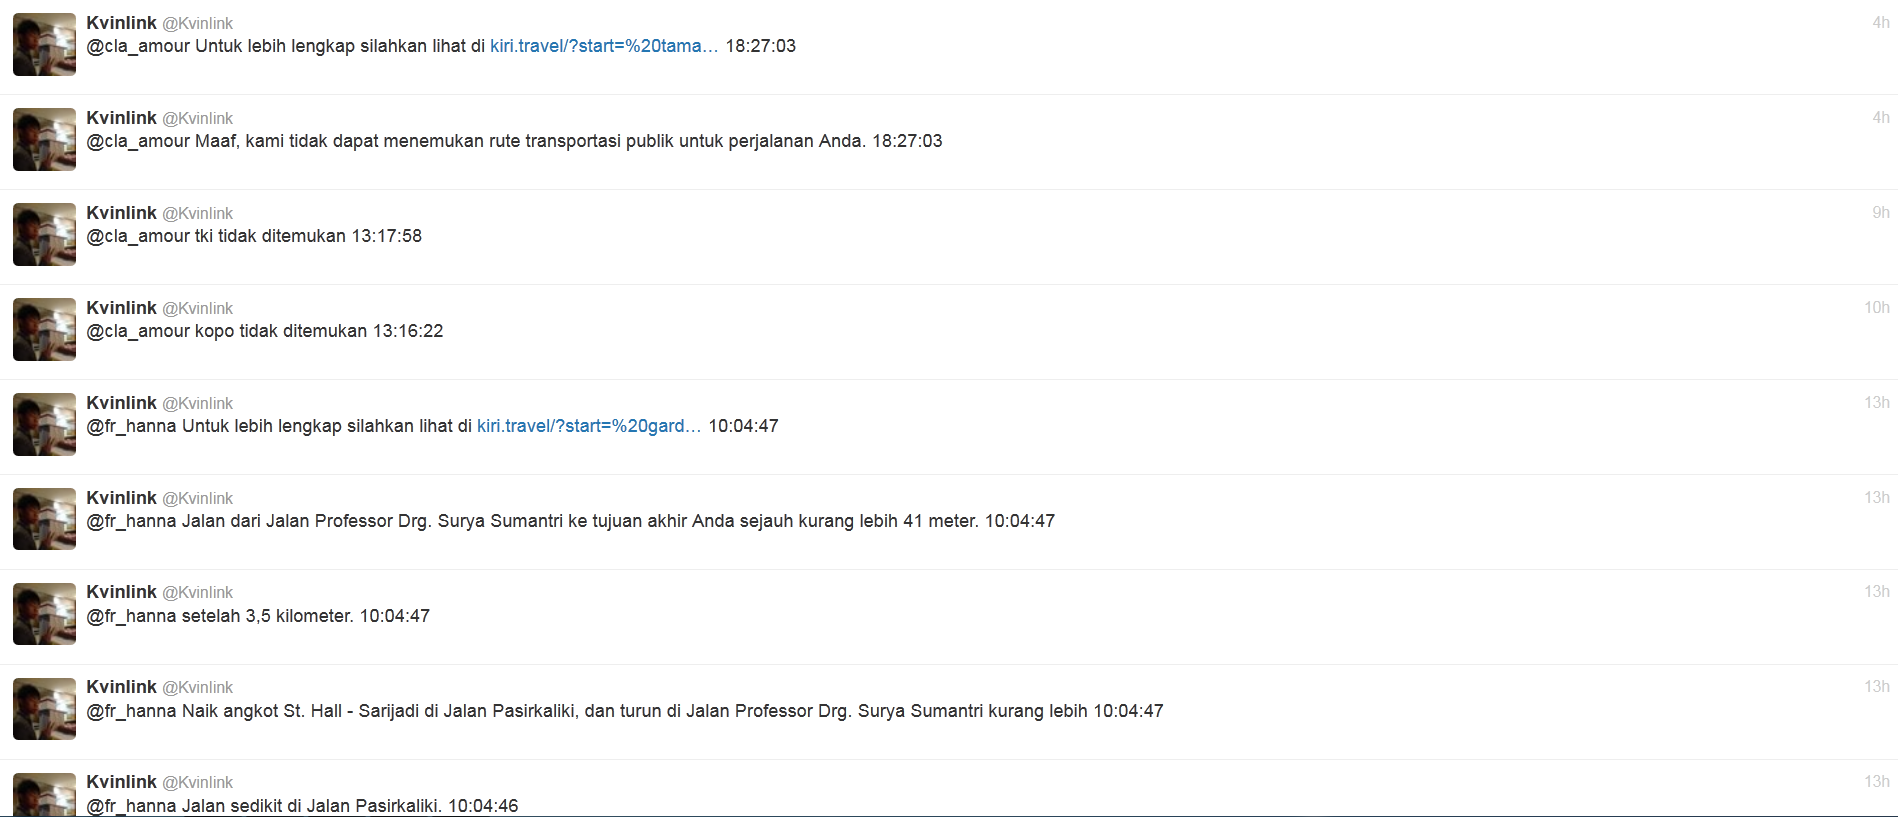
\includegraphics[width=0.9\textwidth]{C:/Skripsi/doc/DokumenSkripsi/Gambar/HasilFinal1.PNG}
		\caption{Hasil Reply Twitter Bot}
		\label{fig:HasilFinal1}
	\end{figure}
	
	\begin{figure}
		\centering
			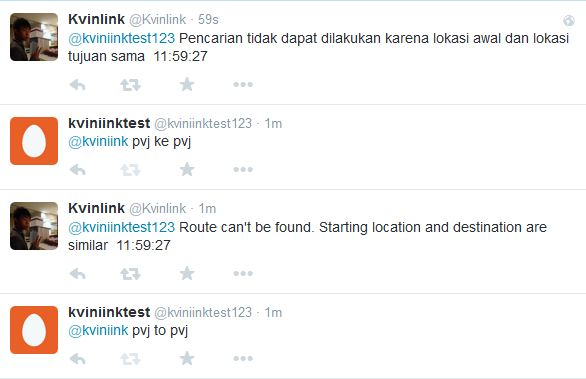
\includegraphics[width=0.9\textwidth]{C:/Skripsi/doc/DokumenSkripsi/Gambar/HasilTweetSama.JPG}
		\caption{Hasil \textit{Tweet} Jika Lokasi Awal dan Lokasi Tujuan Sama}
		\label{fig:HasilTweetSama}
	\end{figure}
	
	\begin{figure}
		\centering
			
\includegraphics[width=0.9\textwidth]{C:/Skripsi/doc/DokumenSkripsi/Gambar/testTweet.PNG}
		\caption{Akun \textit{Twitter Bot} Mendapat Banyak Mention Dalam Satu \textit{Tweet}}
		\label{fig:testTweet}
	\end{figure}
	
	\begin{figure}
		\centering
			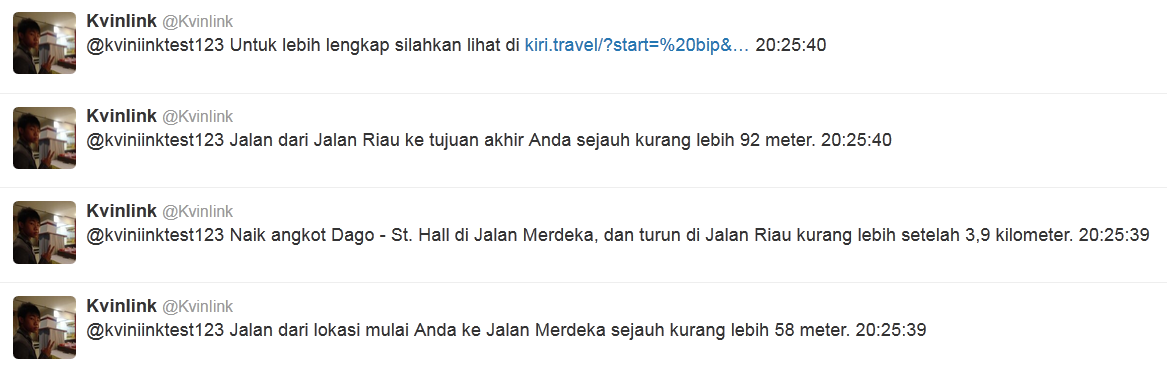
\includegraphics[width=0.9\textwidth]{C:/Skripsi/doc/DokumenSkripsi/Gambar/hasilTestTweet.PNG}
		\caption{Hasil Reply \textit{Twitter Bot}}
		\label{fig:hasilTestTweet}
	\end{figure}
	
	\begin{figure}
		\centering
			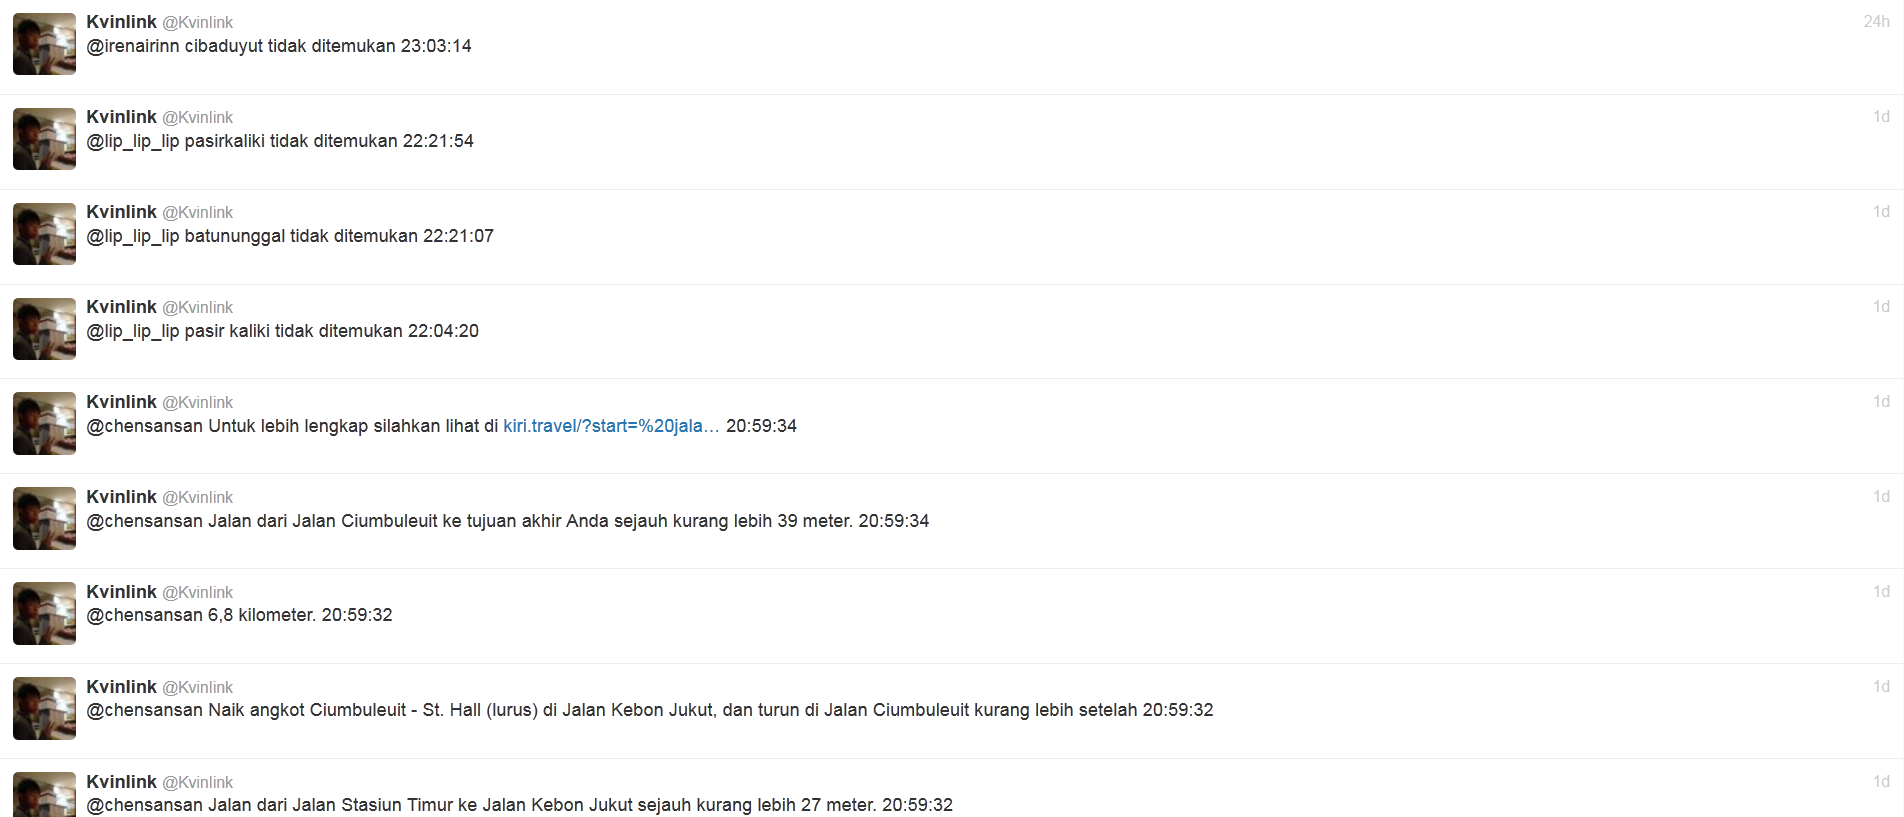
\includegraphics[width=0.9\textwidth]{C:/Skripsi/doc/DokumenSkripsi/Gambar/HasilFinal2.PNG}
			\caption{Hasil Reply \textit{Twitter Bot}}
		\label{fig:HasilFinal2}
	\end{figure}
	
	\begin{figure}
		\centering
			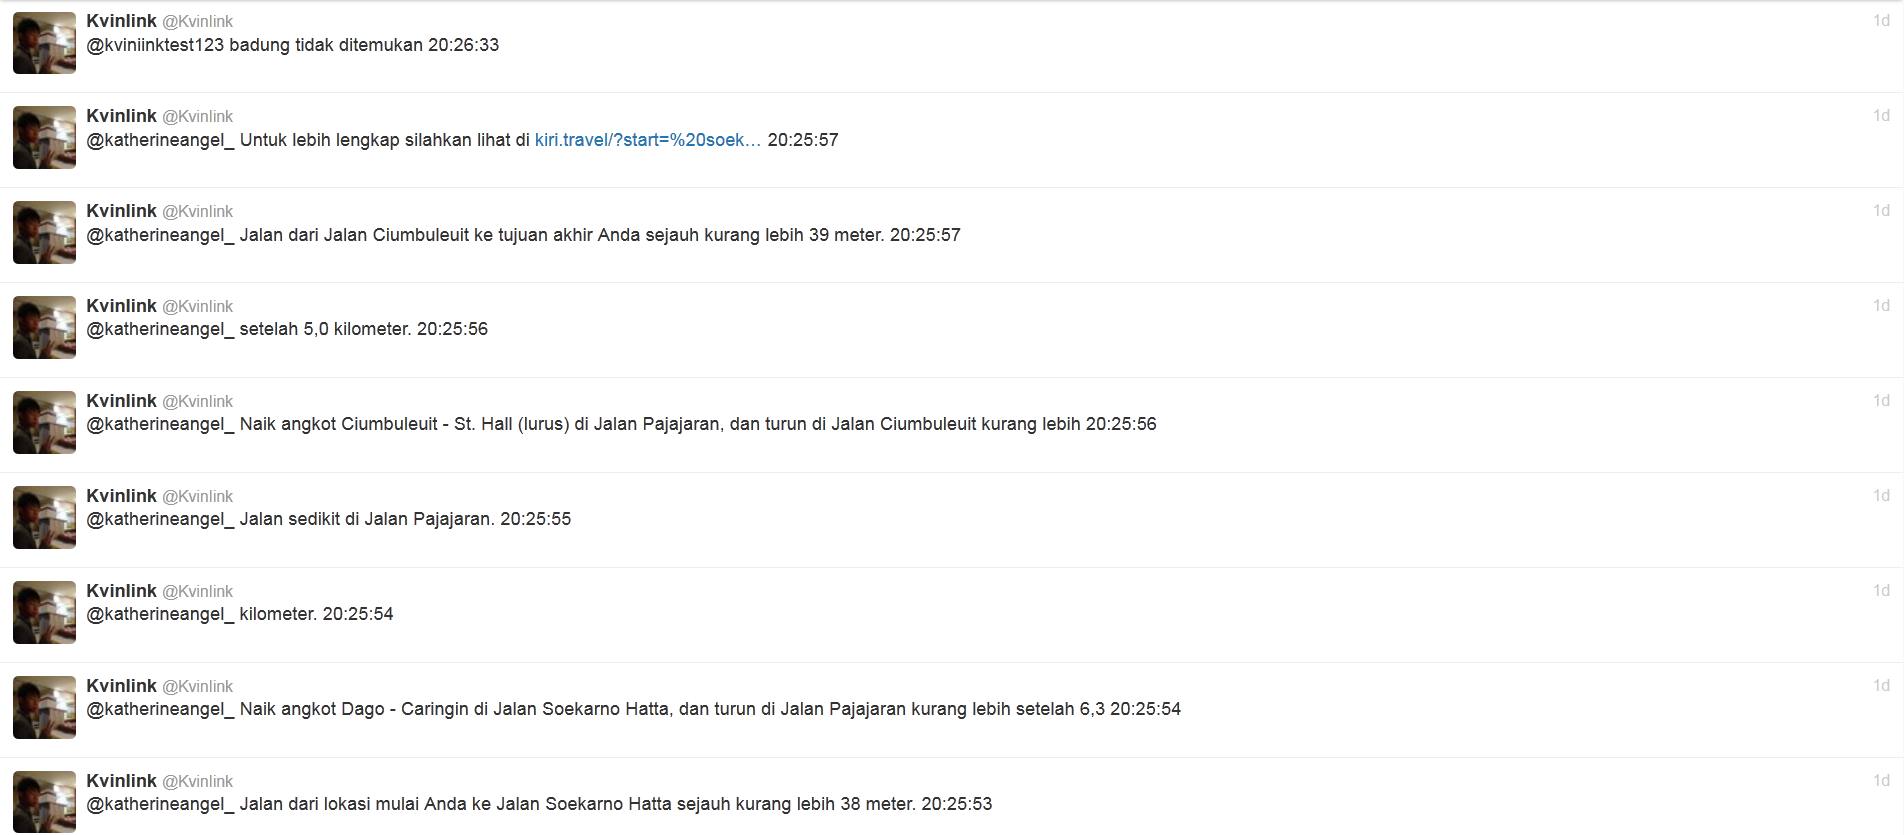
\includegraphics[width=0.9\textwidth]{C:/Skripsi/doc/DokumenSkripsi/Gambar/HasilFinal3.PNG}
			\caption{Hasil Reply \textit{Twitter Bot}}
		\label{fig:HasilFinal3}
	\end{figure}
	
	\clearpage
	\item Pengujian 3
	
	Pada pengujian tiga dilakukan pengujian untuk mengetahui apakah hasil \textit{tweet} yang diberikan \textit{Twitter bot} terdapat kesalahan atau tidak jika \textit{Twitter bot} mendapatkan dua \textit{tweet} atau lebih pada waktu yang bersamaan. Pengujian dilakukan dengan cara melakukan dua \textit{tweet} pencarian secara bersamaan. Penulis meminta bantuan kepada beberapa responden untuk melakukan \textit{tweet} pencarian secara bersamaan. Hasil pengujian untuk \textit{tweet} pencarian yang dilakukan secara bersamaan dapat dilihat pada tabel~\ref{tab:tabelHasilPengujianTweetYangDilakukanSecaraBersamaan}.
	
	\begin{table}[h]
	\caption{Tabel 1 hasil pengujian \textit{tweet} yang dilakukan secara bersamaan}
	\label{tab:tabelHasilPengujianTweetYangDilakukanSecaraBersamaan}
		\begin{tabular}{|p{0.5cm}|p{2.5cm}|p{1.5cm}|p{4cm}|p{6cm}|}
			\hline
				No & Akun penguji & Waktu \textit{tweet} & \textit{Tweet} yang dikirimkan pengguna & \textit{Tweet} yang diterima pengguna \\ \hline
				1 & @ClaraKwaria & 10:49 &  @KvinIink UNPAR to PVJ & 
				\begin{itemize}
					\item @ClaraKwaria Walk about 44 meter from your starting point to Jalan Ciumbuleuit. 22:49:19
					\item @ClaraKwaria Take angkot Ciumbuleuit - St. Hall (belok) at Jalan Ciumbuleuit, and alight at Jalan Sederhana about 2.4 kilometer 22:49:20
					\item @ClaraKwaria later. 22:49:20
					\item @ClaraKwaria Walk about 460 meter from Jalan Sederhana to your destination. 22:49:20
					\item @ClaraKwaria For futher information you can visit http:\/\/kiri.travel?start=unpar \&finish=pvj\&region=bdo 22:49:20
				\end{itemize} \\ \hline
				2 & @clara00010111 & 10:49 &  @KvinIink UNPAR to PVJ &
				\begin{itemize}
					\item @clara00010111 Walk about 44 meter from your starting point to Jalan Ciumbuleuit. 22:49:23 
					\item @clara00010111 Take angkot Ciumbuleuit - St. Hall (belok) at Jalan Ciumbuleuit, and alight at Jalan Sederhana about 2.4 kilometer 22:49:23
					\item @clara00010111 later. 22:49:23
					\item @clara00010111 Walk about 460 meter from Jalan Sederhana to your destination. 22:49:24
					\item @clara00010111 For futher information you can visit http:\/\/kiri.travel?start=unpar \&finish=pvj\&region=bdo 22:49:24
				\end{itemize} \\ \hline
		\end{tabular}
\end{table}

\begin{table}[h]
	\caption{Tabel 2 hasil pengujian \textit{tweet} yang dilakukan secara bersamaan}
	\label{tab:tabelHasilPengujianTweetYangDilakukanSecaraBersamaan}
		\begin{tabular}{|p{0.5cm}|p{2.5cm}|p{1.5cm}|p{4cm}|p{6cm}|}
			\hline
				No & Akun penguji & Waktu \textit{tweet} & \textit{Tweet} yang dikirimkan pengguna & \textit{Tweet} yang diterima pengguna \\ \hline
				3 & @ClaraKwaria & 10:52 &  @KvinIink UNPAR ke PVJ &
				\begin{itemize}
					\item @clara00010111 Jalan dari lokasi mulai Anda ke Jalan Ciumbuleuit sejauh kurang lebih 44 meter. 22:52:37
					\item @clara00010111 Naik angkot Ciumbuleuit - St. Hall (belok) di Jalan Ciumbuleuit, dan turun di Jalan Sederhana kurang lebih setelah 22:52:38
					\item @clara00010111 2,4 kilometer. 22:52:38
					\item @clara00010111 Jalan dari Jalan Sederhana ke tujuan akhir Anda sejauh kurang lebih 460 meter. 22:52:39
					\item @clara00010111 Untuk lebih lengkapnya dapat dilihat pada http:\/\/kiri.travel?start=unpar \&finish=pvj\&region=bdo 22:52:39 
				\end{itemize} \\ \hline
				4 & @clara00010111 & 10:52 &  @KvinIink UNPAR ke PVJ &
				\begin{itemize}
					\item @clara00010111 Jalan dari lokasi mulai Anda ke Jalan Ciumbuleuit sejauh kurang lebih 44 meter. 22:52:34
					\item @clara00010111 Naik angkot Ciumbuleuit - St. Hall (belok) di Jalan Ciumbuleuit, dan turun di Jalan Sederhana kurang lebih setelah 22:52:34
					\item @clara00010111 2,4 kilometer. 22:52:34
					\item @clara00010111 Jalan dari Jalan Sederhana ke tujuan akhir Anda sejauh kurang lebih 460 meter. 22:52:35
					\item @clara00010111 Untuk lebih lengkapnya dapat dilihat pada http:\/\/kiri.travel?start=unpar \&finish=pvj\&region=bdo 22:52:35 
				\end{itemize} \\ \hline
		\end{tabular}
\end{table}

\begin{table}[h]
	\caption{Tabel 3 hasil pengujian \textit{tweet} yang dilakukan secara bersamaan}
	\label{tab:tabelHasilPengujianTweetYangDilakukanSecaraBersamaan}
		\begin{tabular}{|p{0.5cm}|p{2.5cm}|p{1.5cm}|p{4cm}|p{6cm}|}
			\hline
				No & Akun penguji & Waktu \textit{tweet} & \textit{Tweet} yang dikirimkan pengguna & \textit{Tweet} yang diterima pengguna \\ \hline
				5 & @ClaraKwaria & 10:59 &  @KvinIink UNPAR ke BIP &
				\begin{itemize}
					\item @ClaraKwaria Jalan dari lokasi mulai Anda ke Jalan Ciumbuleuit sejauh kurang lebih 44 meter. 23:00:04
					\item @ClaraKwaria Naik angkot Ciumbuleuit - St. Hall (lurus) di Jalan Ciumbuleuit, dan turun di Jalan Cihampelas kurang lebih setelah 23:00:04
					\item @ClaraKwaria 3,3 kilometer. 23:00:04
					\item @ClaraKwaria Jalan dari Jalan Cihampelas ke Jalan Wastukancana sejauh kurang lebih 17 meter. 23:00:05
					\item @ClaraKwaria Naik angkot Ciroyom - Antapani di Jalan Wastukancana, dan turun di Jalan Aceh kurang lebih setelah 1,4 kilometer. 23:00:06
					\item @ClaraKwaria Jalan dari Jalan Aceh ke tujuan akhir Anda sejauh kurang lebih 124 meter. 23:00:06
					\item @ClaraKwaria Untuk lebih lengkapnya dapat dilihat pada http:\/\/kiri.travel?start=unpar \&finish=bip\&region=bdo 23:00:02 23:00:06
				\end{itemize} \\ \hline
		\end{tabular}
\end{table}

\begin{table}[h]
	\caption{Tabel 4 hasil pengujian \textit{tweet} yang dilakukan secara bersamaan}
	\label{tab:tabelHasilPengujianTweetYangDilakukanSecaraBersamaan}
		\begin{tabular}{|p{0.5cm}|p{2.5cm}|p{1.5cm}|p{4cm}|p{6cm}|}
			\hline
				No & Akun penguji & Waktu \textit{tweet} & \textit{Tweet} yang dikirimkan pengguna & \textit{Tweet} yang diterima pengguna \\ \hline
				6 & @clara00010111 & 10:59 &  @KvinIink UNPAR to BIP &
				\begin{itemize}
					\item @clara00010111 Walk about 44 meter from your starting point to Jalan Ciumbuleuit. 22:59:59
					\item @clara00010111 Take angkot Ciumbuleuit - St. Hall (lurus) at Jalan Ciumbuleuit, and alight at Jalan Cihampelas about 3.3 kilometer 23:00:00
					\item @clara00010111 later. 23:00:00
					\item @clara00010111 Walk about 17 meter from Jalan Cihampelas to Jalan Wastukancana. 23:00:01
					\item @clara00010111 Take angkot Ciroyom - Antapani at Jalan Wastukancana, and alight at Jalan Aceh about 1.4 kilometer later. 23:00:01
					\item @clara00010111 Walk about 124 meter from Jalan Aceh to your destination. 23:00:02
					\item @clara00010111 For futher information you can visit http:\/\/kiri.travel?start=unpar \&finish=bip\&region=bdo 23:00:02
				\end{itemize} \\ \hline
				7 & @ClaraKwaria & 10:02 &  @KvinIink bantuan &
				\begin{itemize}
					\item @ClaraKwaria Format penggunaan \textit{Twitter bot} untuk mencari jalur transportasi publik adalah... 23:00:06
					\item @ClaraKwaria 'Lokasi awal' ke 'lokasi tujuan', contoh : BIP ke PVJ. 23:00:06
				\end{itemize} \\ \hline
				8 & @clara00010111 & 10:02 &  @KvinIink help &
				\begin{itemize}
					\item @clara00010111 For using this \textit{Twitter bot} for searching public transport route, you can mention... 23:00:06
					\item @clara00010111 'First location' to 'second location', example : BIP to PVJ 23:00:06
				\end{itemize} \\ \hline
		\end{tabular}
\end{table}

\end{enumerate}}{}

%\bibliographystyle{ieeetr}
%\bibliography{pustaka}
\begin{thebibliography}{1}
	\bibitem{Twitter} Twitter {\em Twitter Documentation} 2014 : \url{https://dev.twitter.com/overview/documentation}.
	\bibitem{TwitterBook} Tim O'Reilly {\em The Twitter Book} 2009: O'Reilly Media, Inc
	\bibitem{KIRI} Kiri Team {\em KIRI API v2 Documentation} 2014 : \url{https://bitbucket.org/projectkiri/kiri\_
api/wiki/KIRI\%20API\%20v2\%20Documentation}
	\bibitem{Twitter4J} Twitter4J {\em Twitter4J Documentation}  2007 : \url{http://twitter4j.org/javadoc/index.html}
	\bibitem{OAuth} OAuth {\em Hueniverse Documentation}  2010 : \url{http://hueniverse.com/oauth/guide/intro/}
\end{thebibliography}

\appendix
\apptoc

\tampillmp{\vlmp}

\end{document}
